\section{Data Quality Checks}


This section documents the basic data quality checks for ALEPH archieved data collected in the LEP1 and LEP2 period. In additional to the raw spectra from the data, jet and particle spectra are compared to the predictions from PYTHIA8 event generator (Version 8.230 Default Tune). 

%The spike in the LEP1 and LEP2 pt spectra near 45 GeV is produced by the particles that took the full beam energy in the transverse plane. The beam energy is 92 GeV so in a two particle configuration each particle will take half of the total energy to conserve various kinematics. 

%%%%%%%%%%%%%%%%%%%%%%%%%%%%%%%%%%%% LEP 1 %%%%%%%%%%%%%%%%%%%%%%%%%%%%%%%%

\subsection{LEP1 Data}

\begin{comment}
\begin{figure}[!htb]
\begin{center}
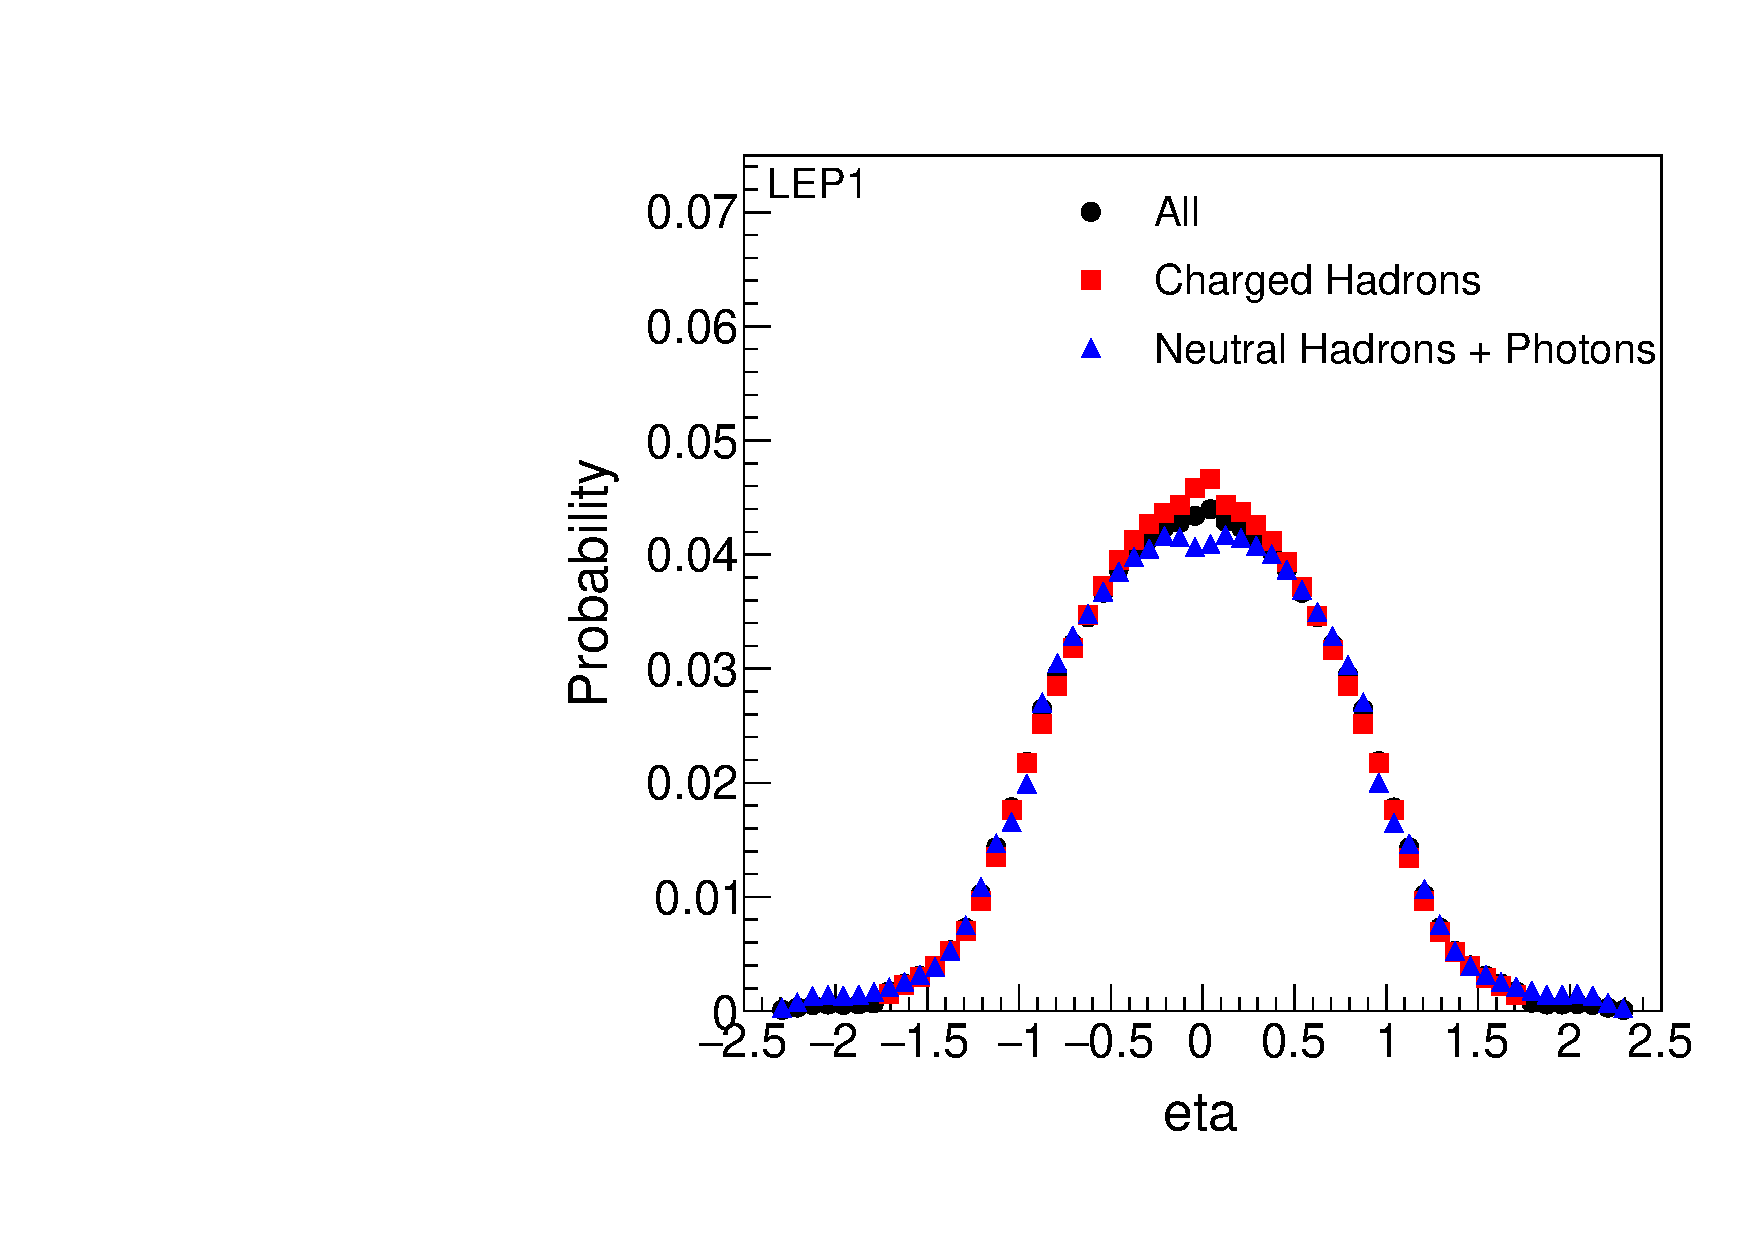
\includegraphics[width=.45\textwidth]{images/DataQualityCheck/LEP1_eta.pdf}
\caption{LEP1 Eta Spectra}
\label{fig:figure1} 
\end{center}
\end{figure}

\begin{figure}[!htb]
\begin{center}
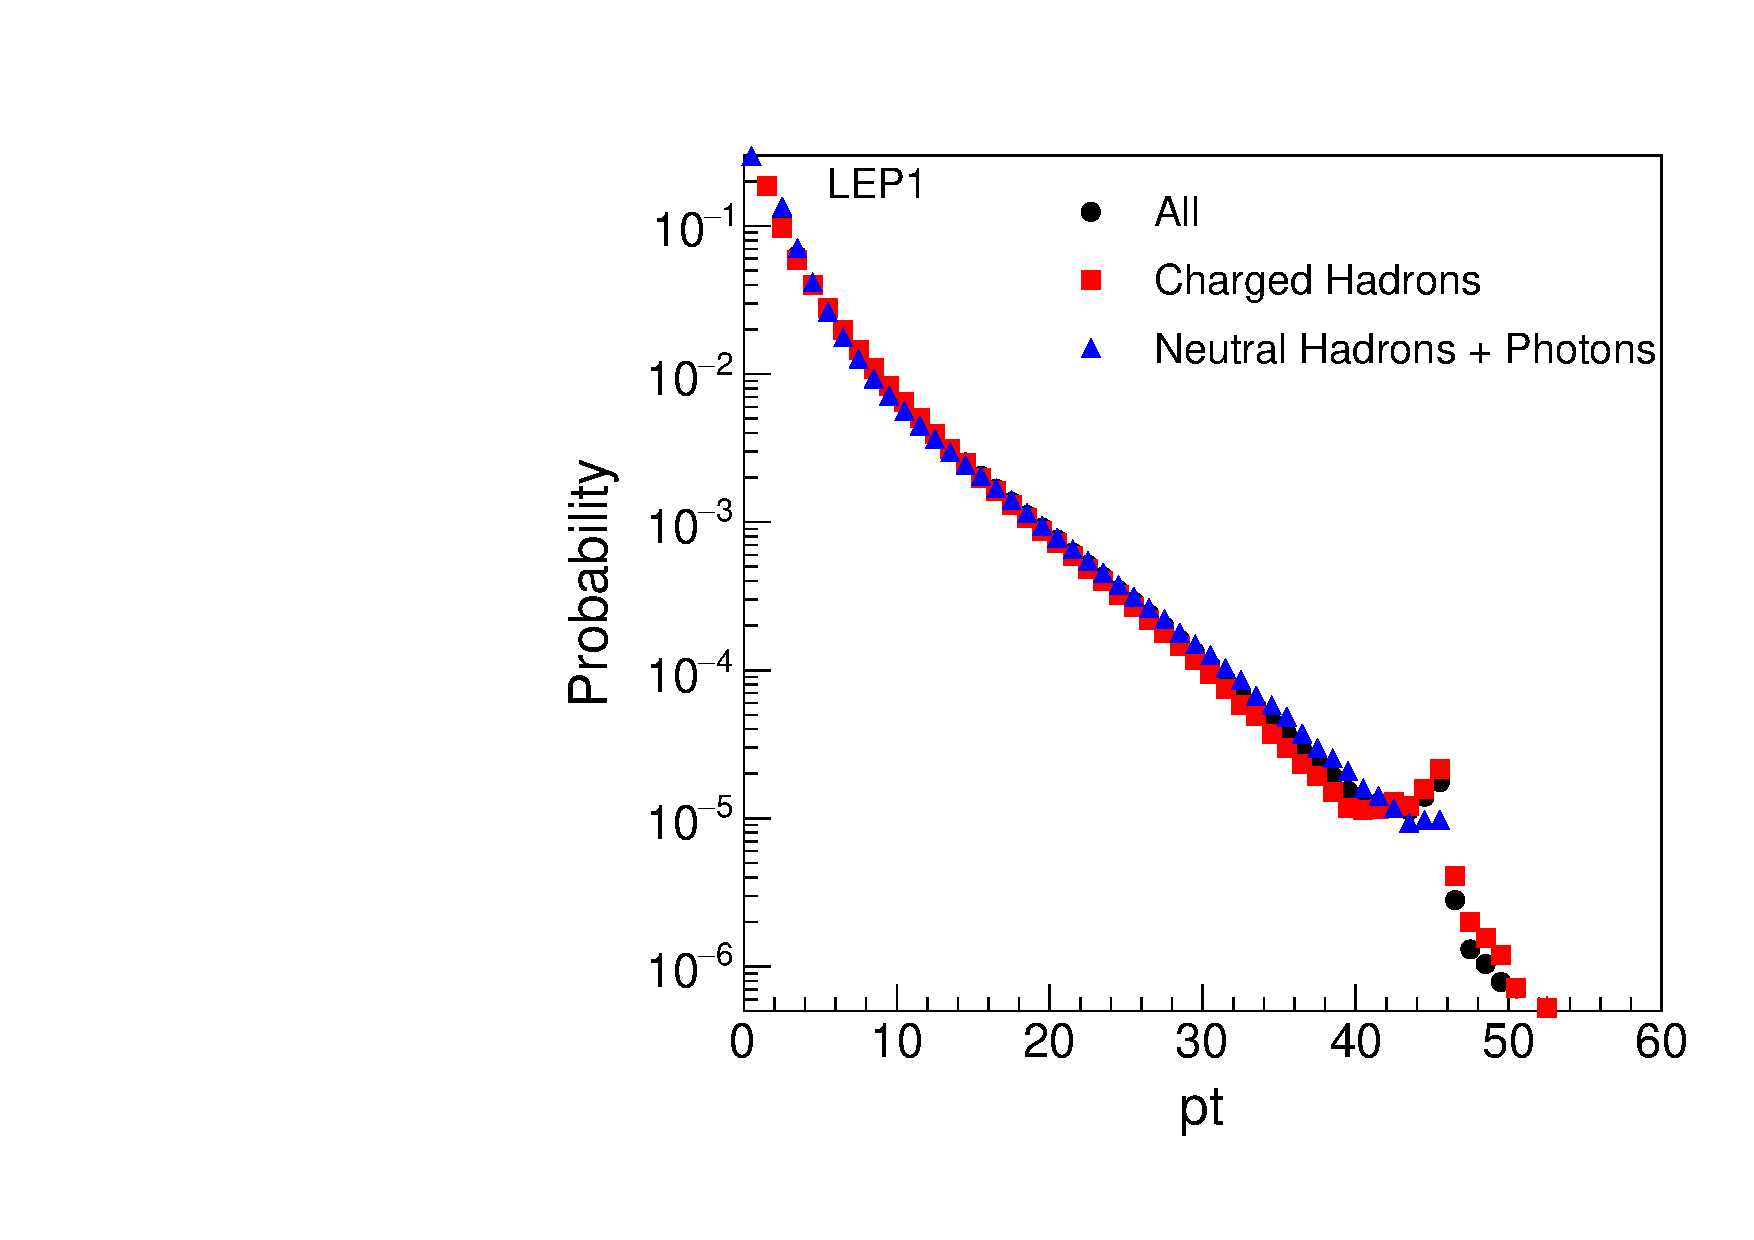
\includegraphics[width=.45\textwidth]{images/DataQualityCheck/LEP1_pt.pdf}
\caption{LEP1 PT spectra}
\label{fig:figure2} 
\end{center}
\end{figure}

\begin{figure}[!htb]
\begin{center}
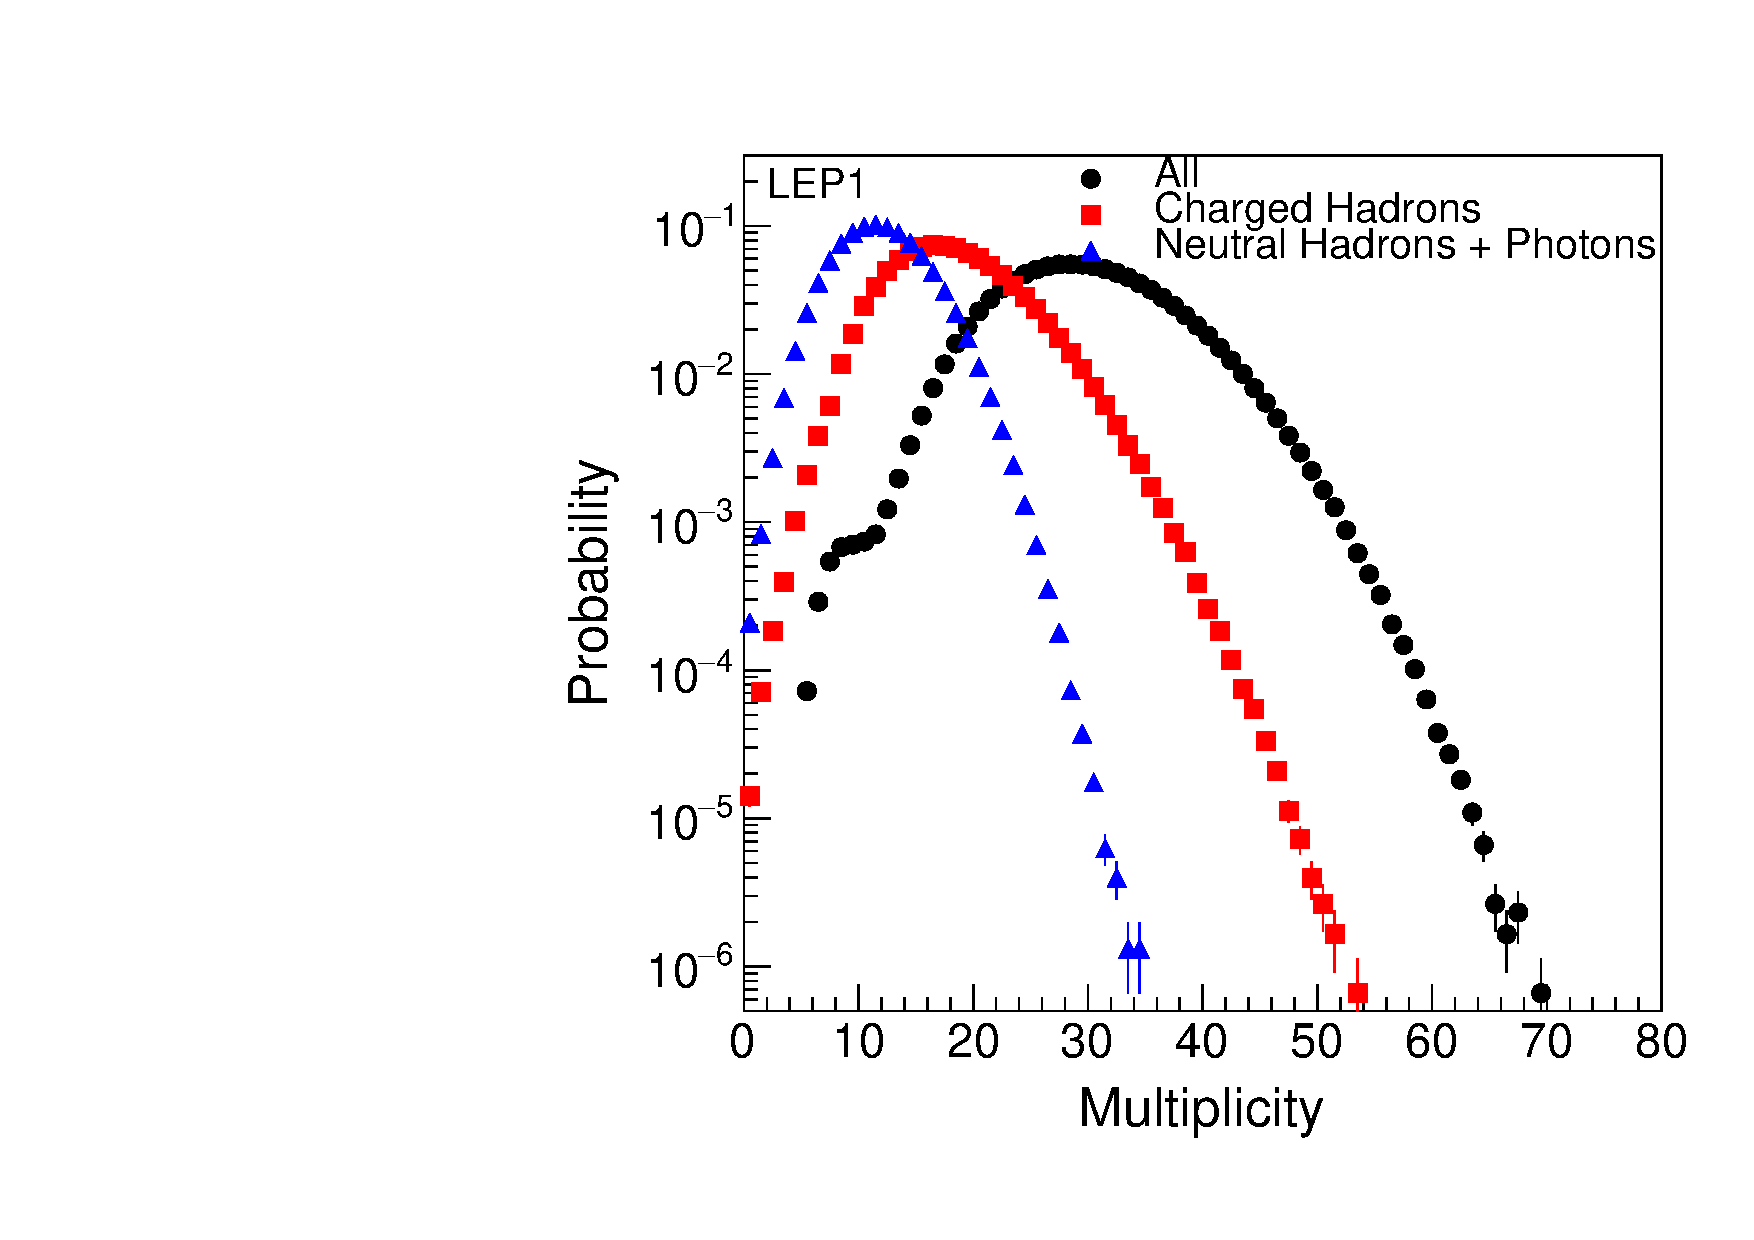
\includegraphics[width=.45\textwidth]{images/DataQualityCheck/LEP1_mult.pdf}
\caption{LEP1 Multiplicity Distribution}
\label{fig:figure6} 
\end{center}
\end{figure}

\begin{figure}[!htb]
\begin{center}
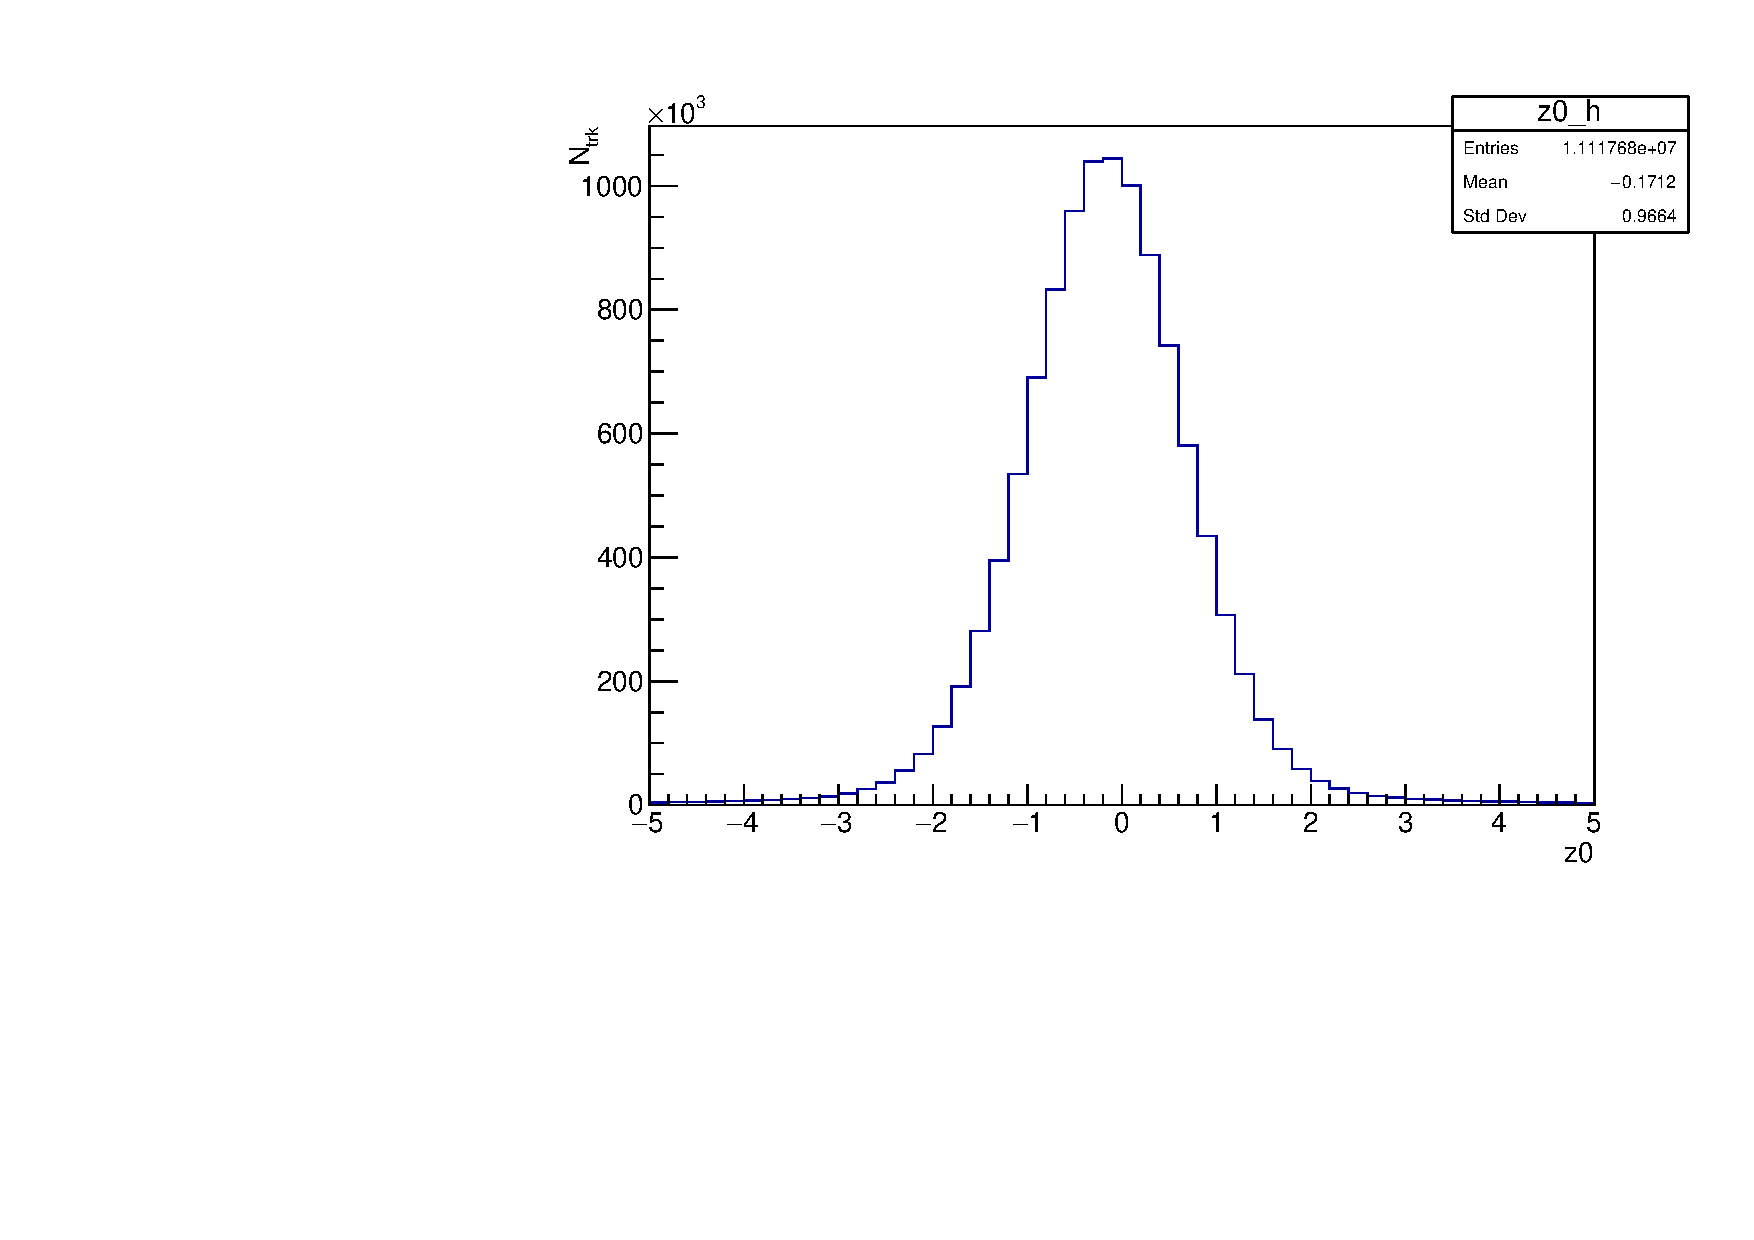
\includegraphics[width=.45\textwidth]{images/DataQualityCheck/z0.pdf}
\caption{LEP1 z distance-of-closest-approach distribution of charged tracks.}
\label{fig:z0} 
\end{center}
\end{figure}

\begin{figure}[!htb]
\begin{center}
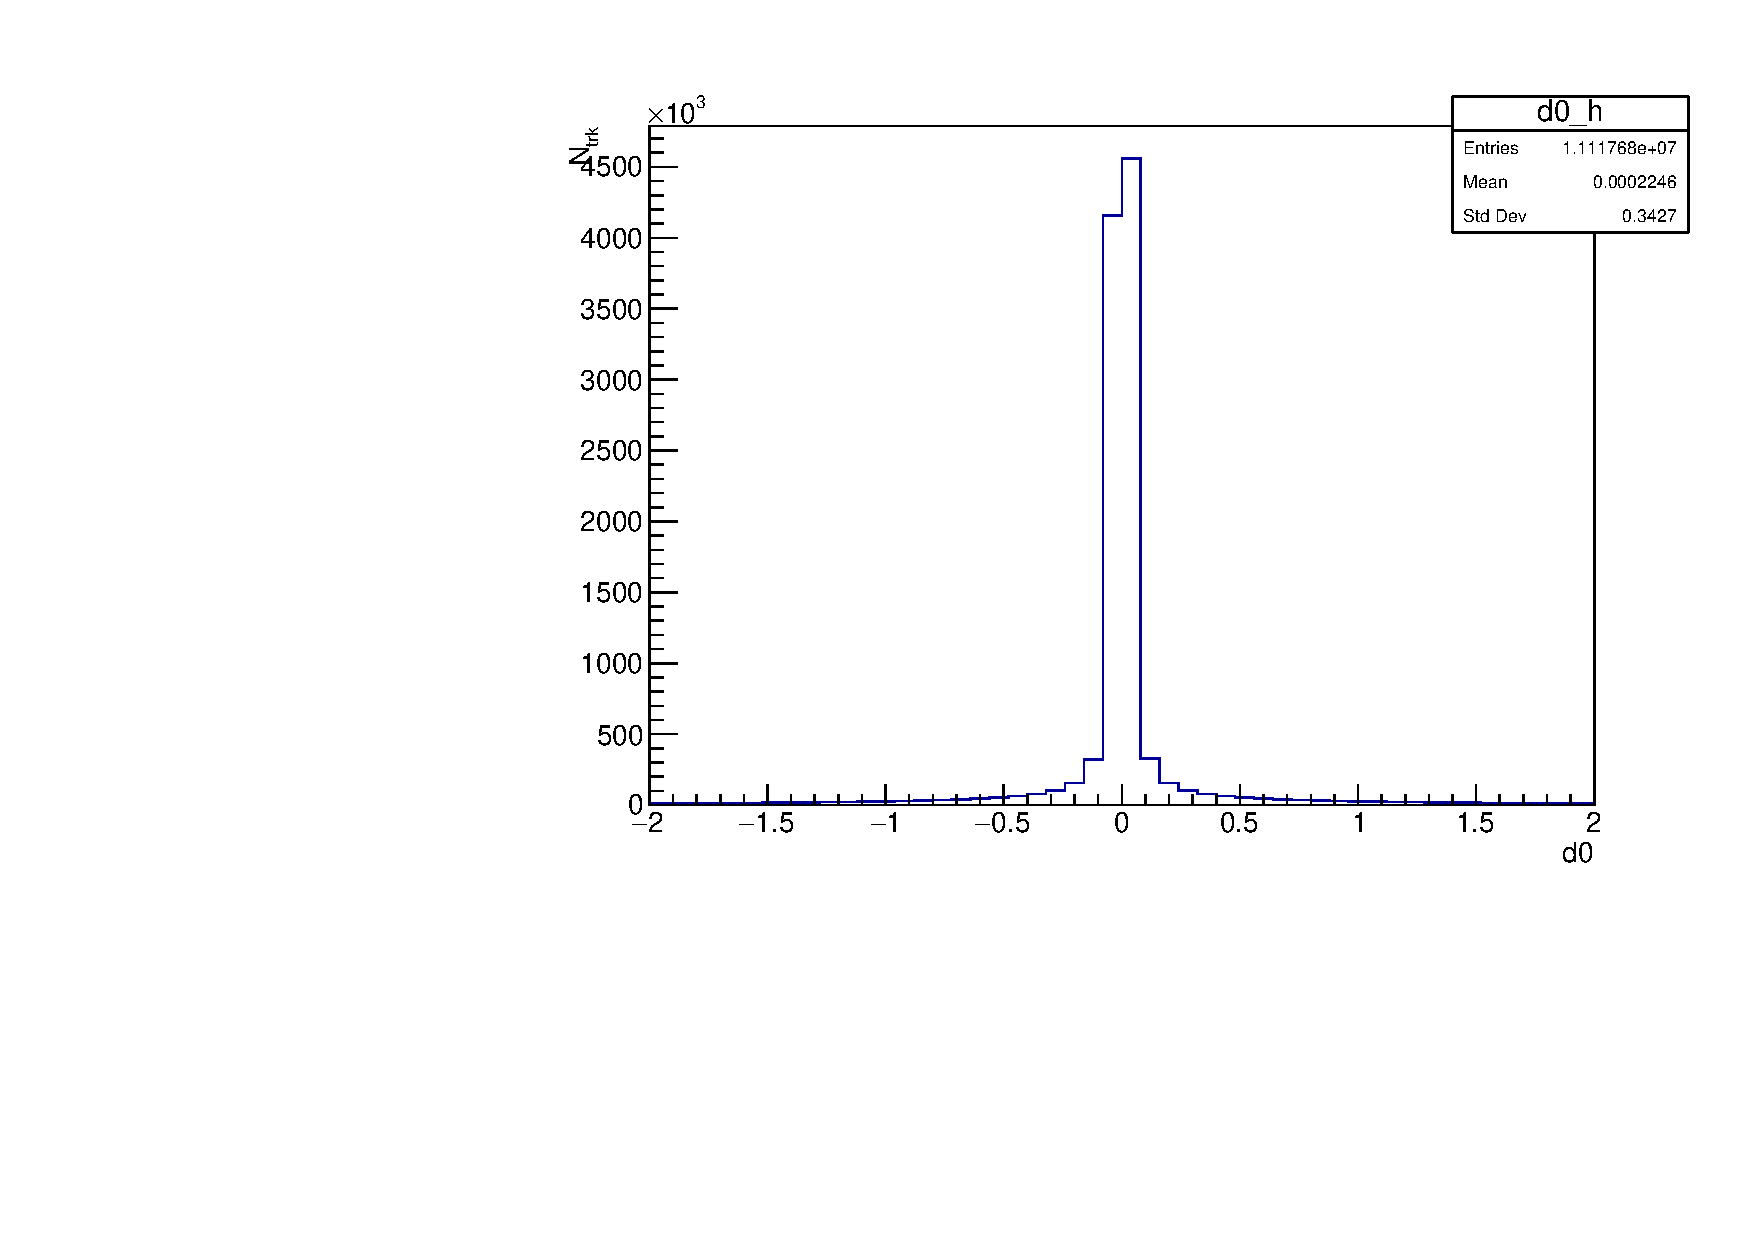
\includegraphics[width=.45\textwidth]{images/DataQualityCheck/d0.pdf}
\caption{LEP1 d0 distribution of charged tracks.}
\label{fig:d0} 
\end{center}
\end{figure}
\begin{figure}[!htb]

\begin{center}
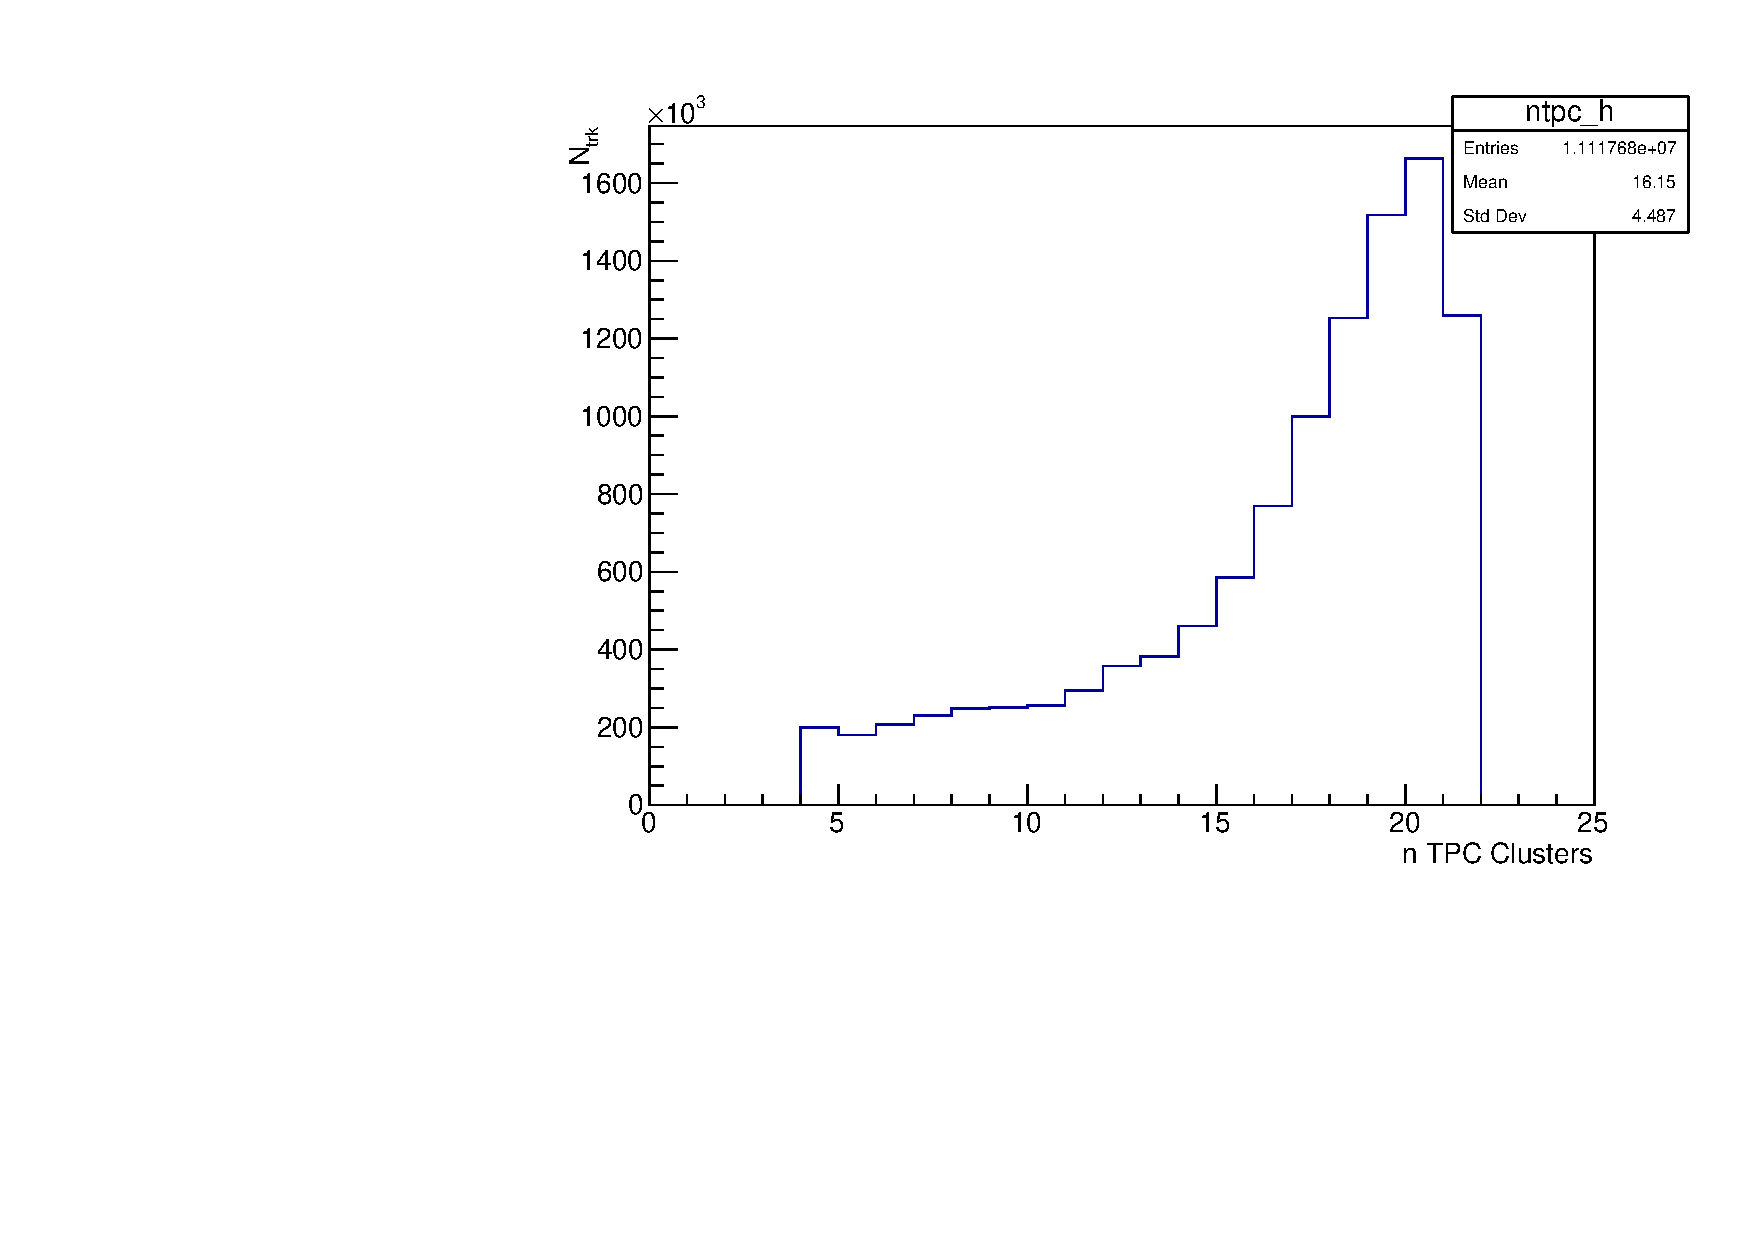
\includegraphics[width=.45\textwidth]{images/DataQualityCheck/ntpc.pdf}
\caption{LEP1 distribution of number of TPC clusters on charged tracks.}
\label{fig:ntpc} 
\end{center}
\end{figure}
\end{comment}

\begin{figure}[H]
\centering
\subfloat{\label{sfig:a}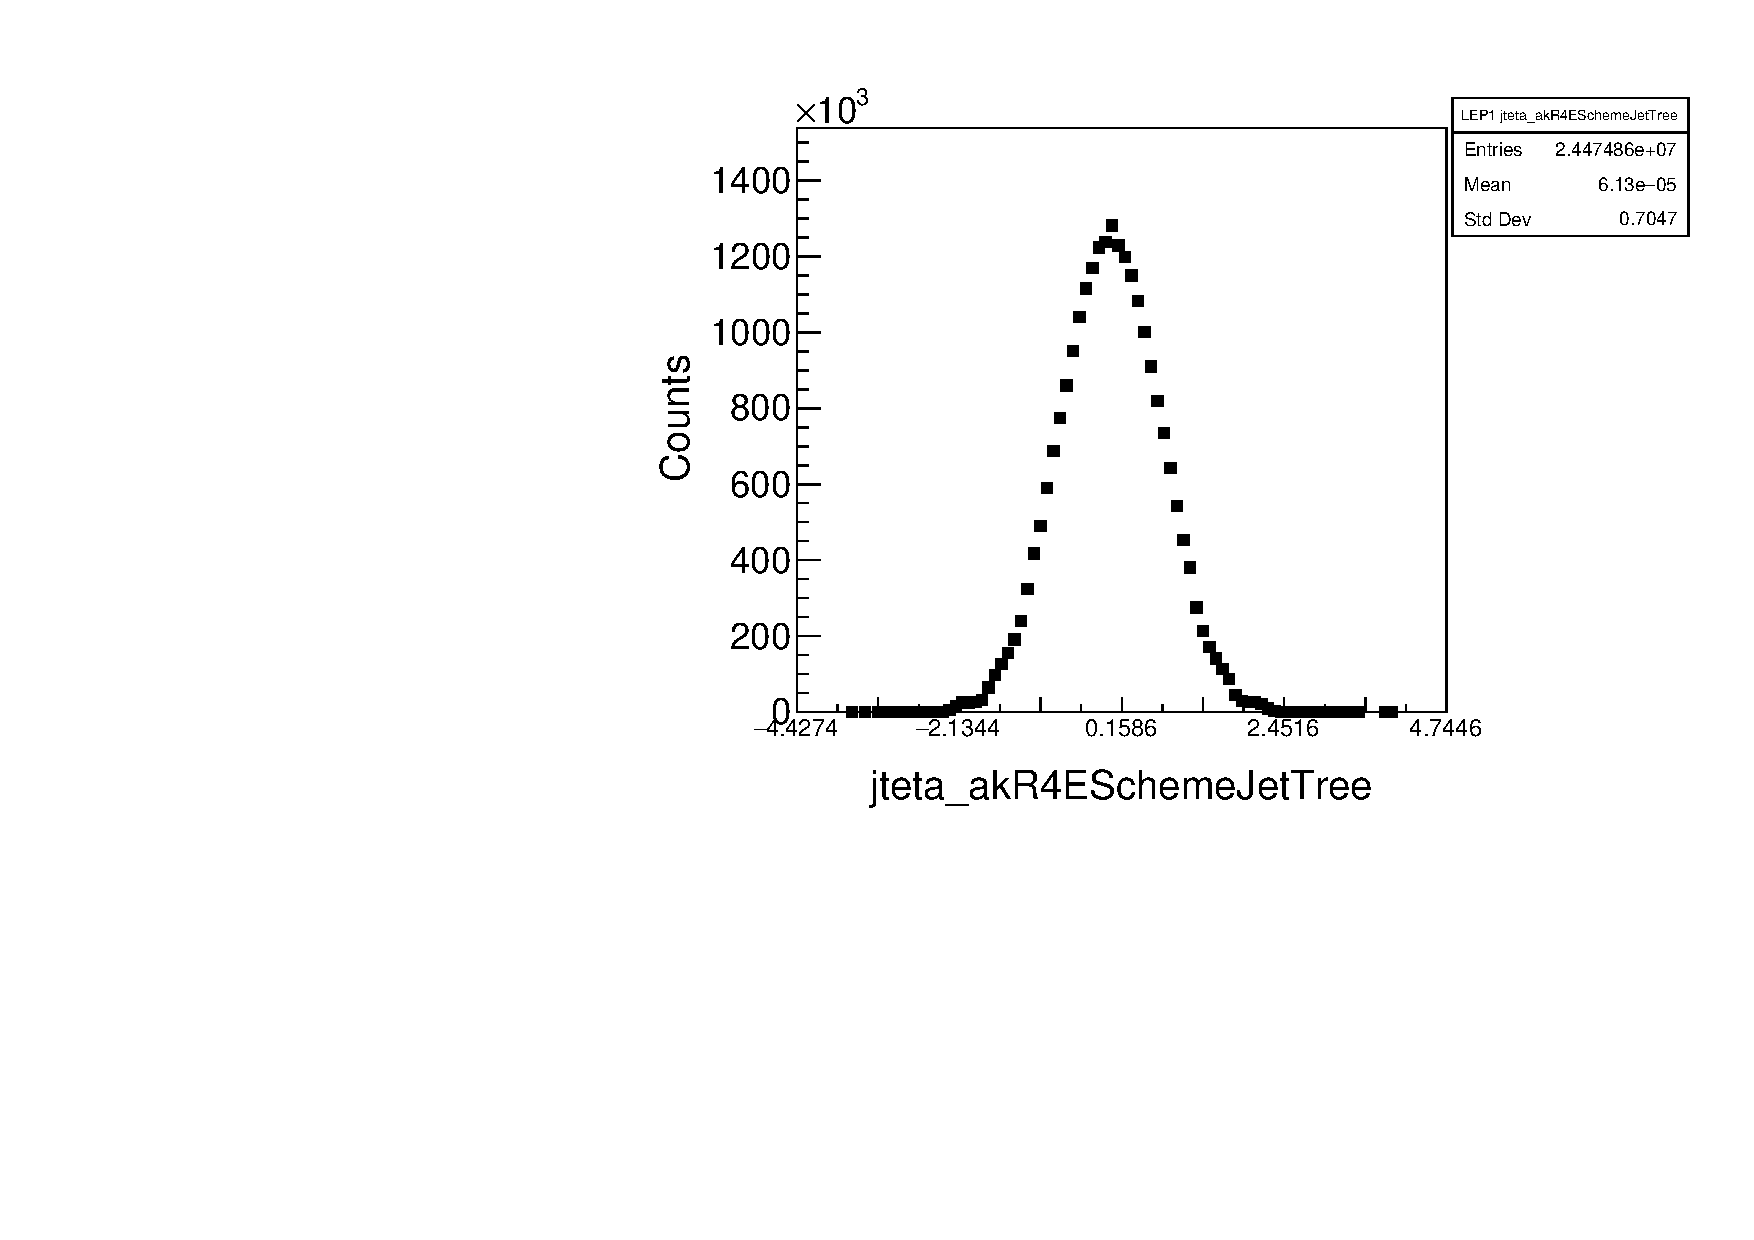
\includegraphics[width=.25\textwidth]{images/DQC/LEP1/jteta_akR4ESchemeJetTree.pdf}}\hfill
\subfloat{\label{sfig:b}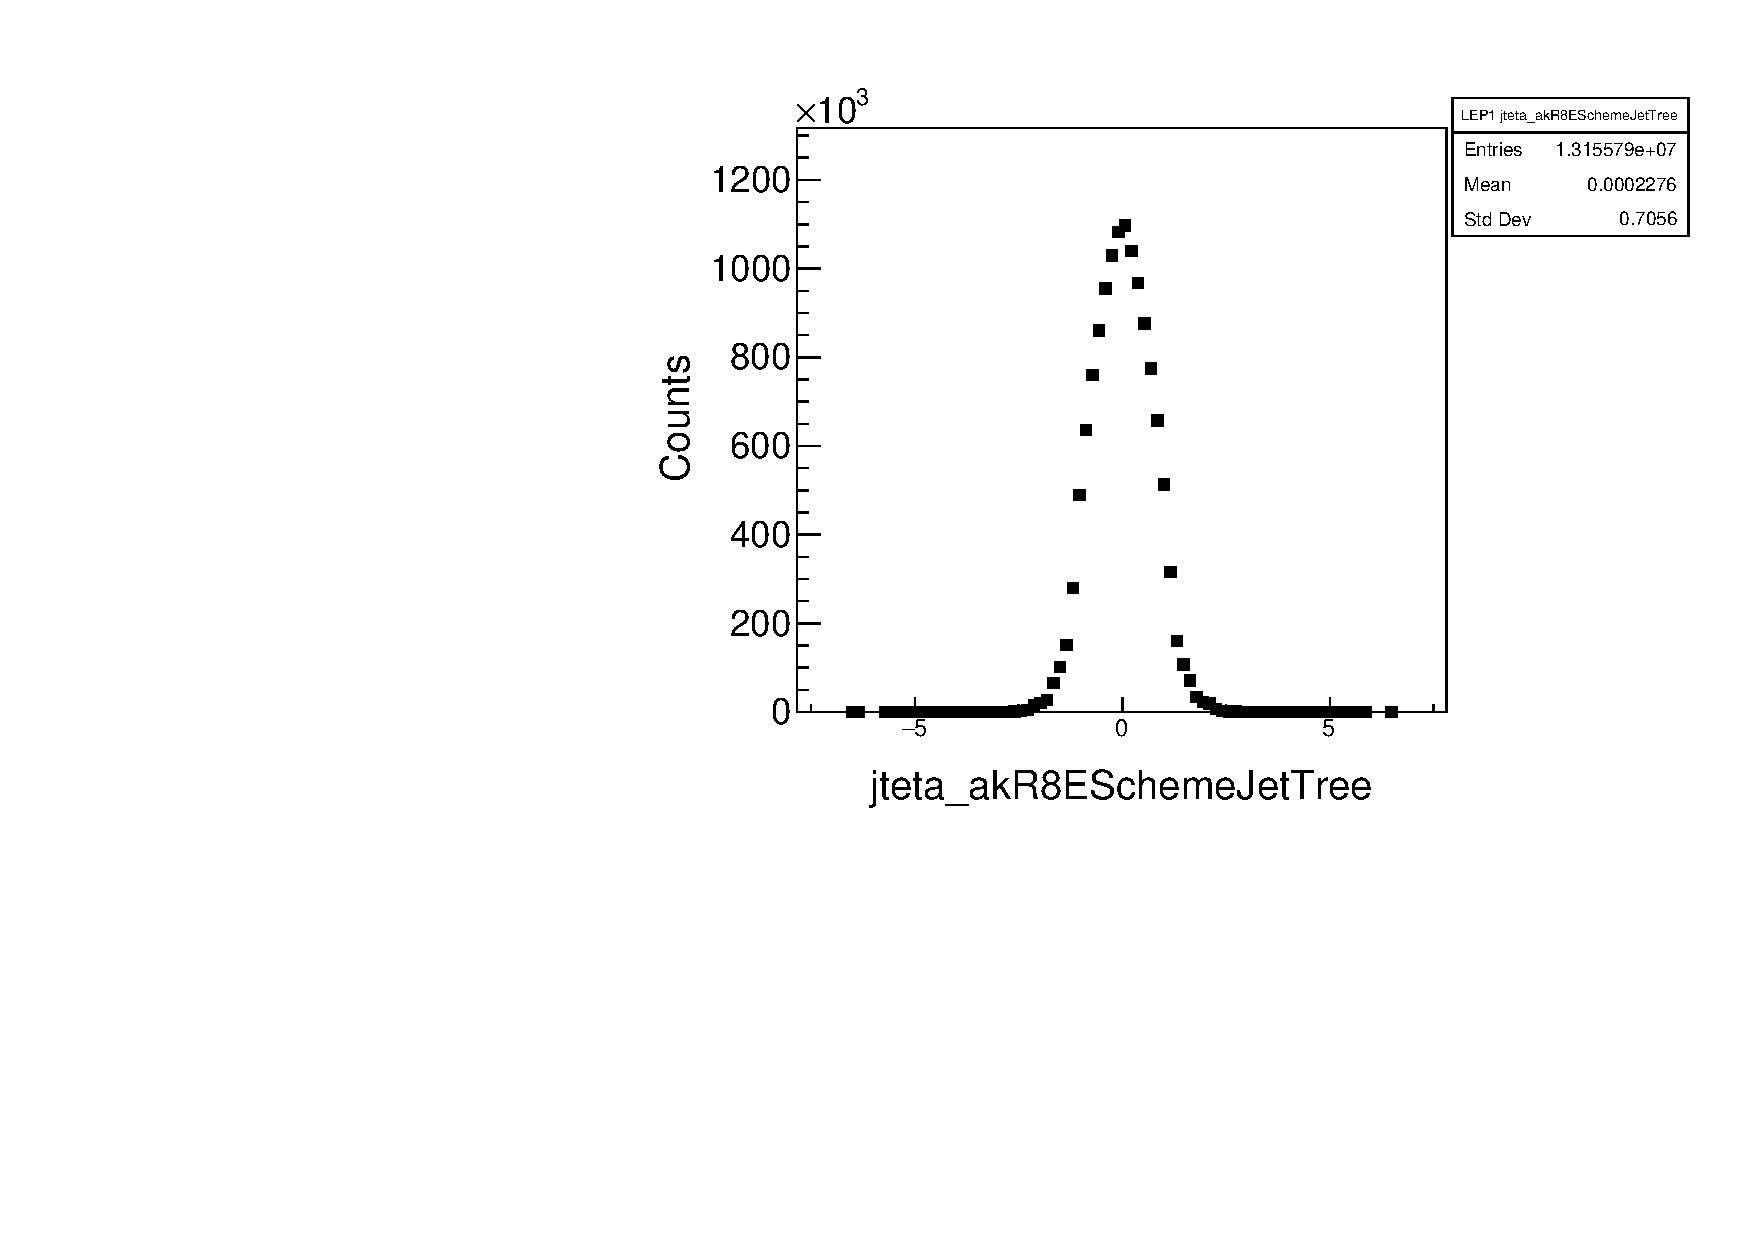
\includegraphics[width=.25\textwidth]{images/DQC/LEP1/jteta_akR8ESchemeJetTree.pdf}}\hfill
\subfloat{\label{sfig:c}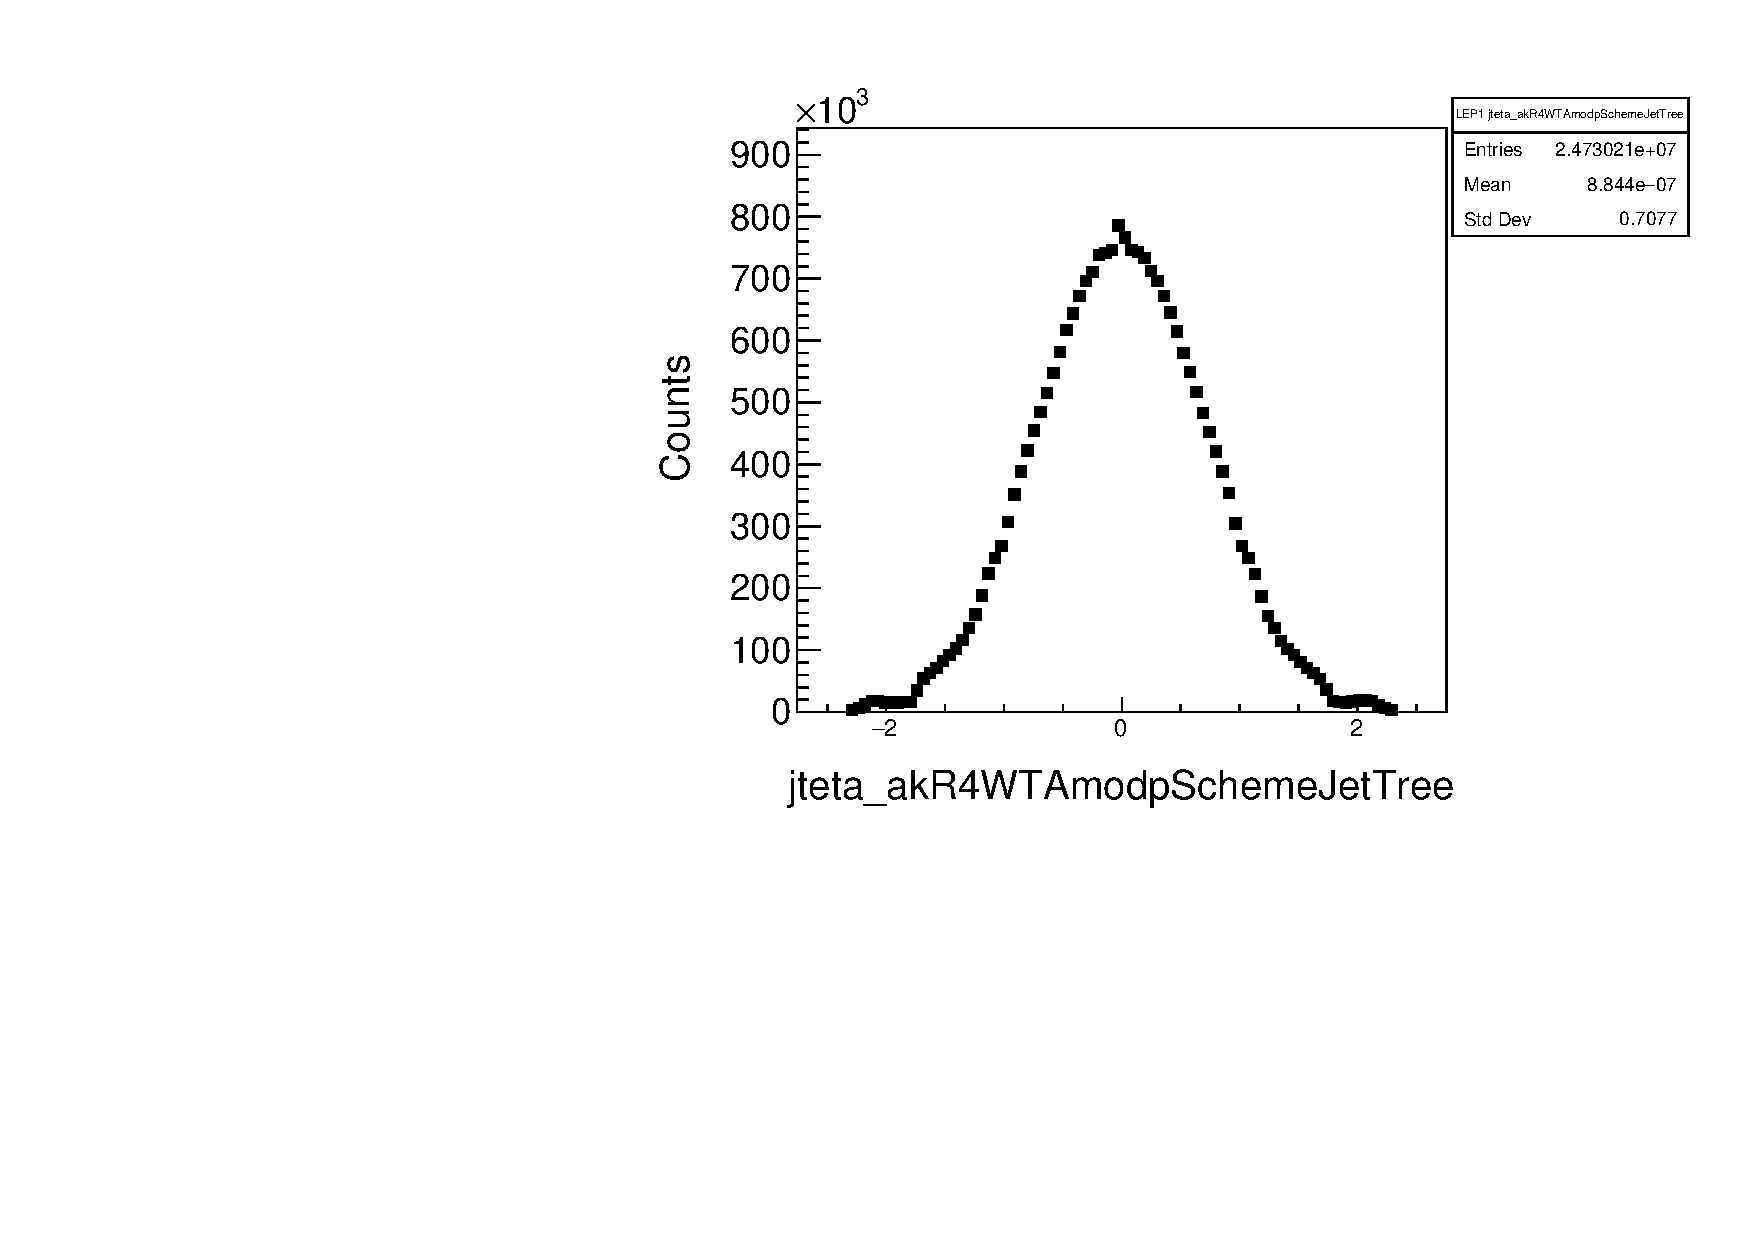
\includegraphics[width=.25\textwidth]{images/DQC/LEP1/jteta_akR4WTAmodpSchemeJetTree.pdf}}\hfill
\subfloat{\label{sfig:d}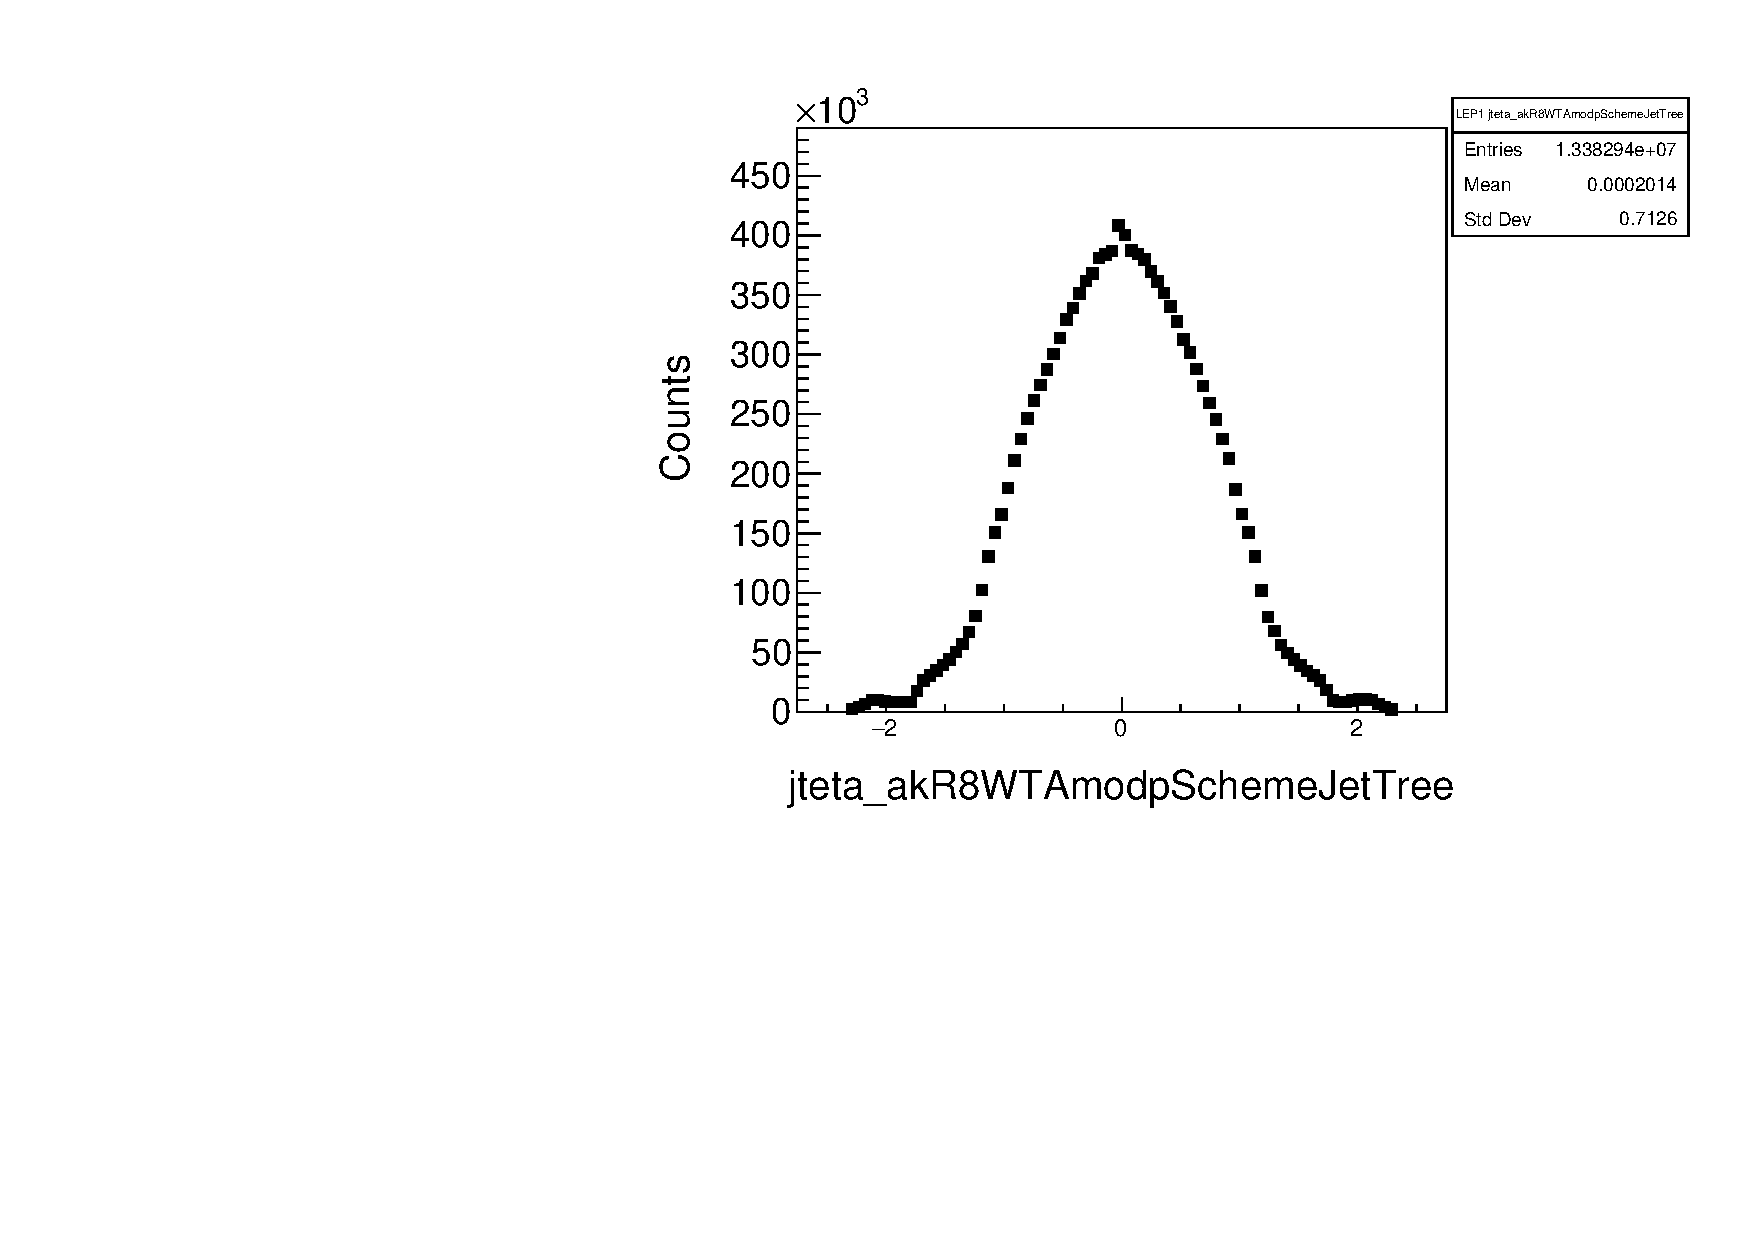
\includegraphics[width=.25\textwidth]{images/DQC/LEP1/jteta_akR8WTAmodpSchemeJetTree.pdf}}\hfill %row end
\subfloat{\label{sfig:e}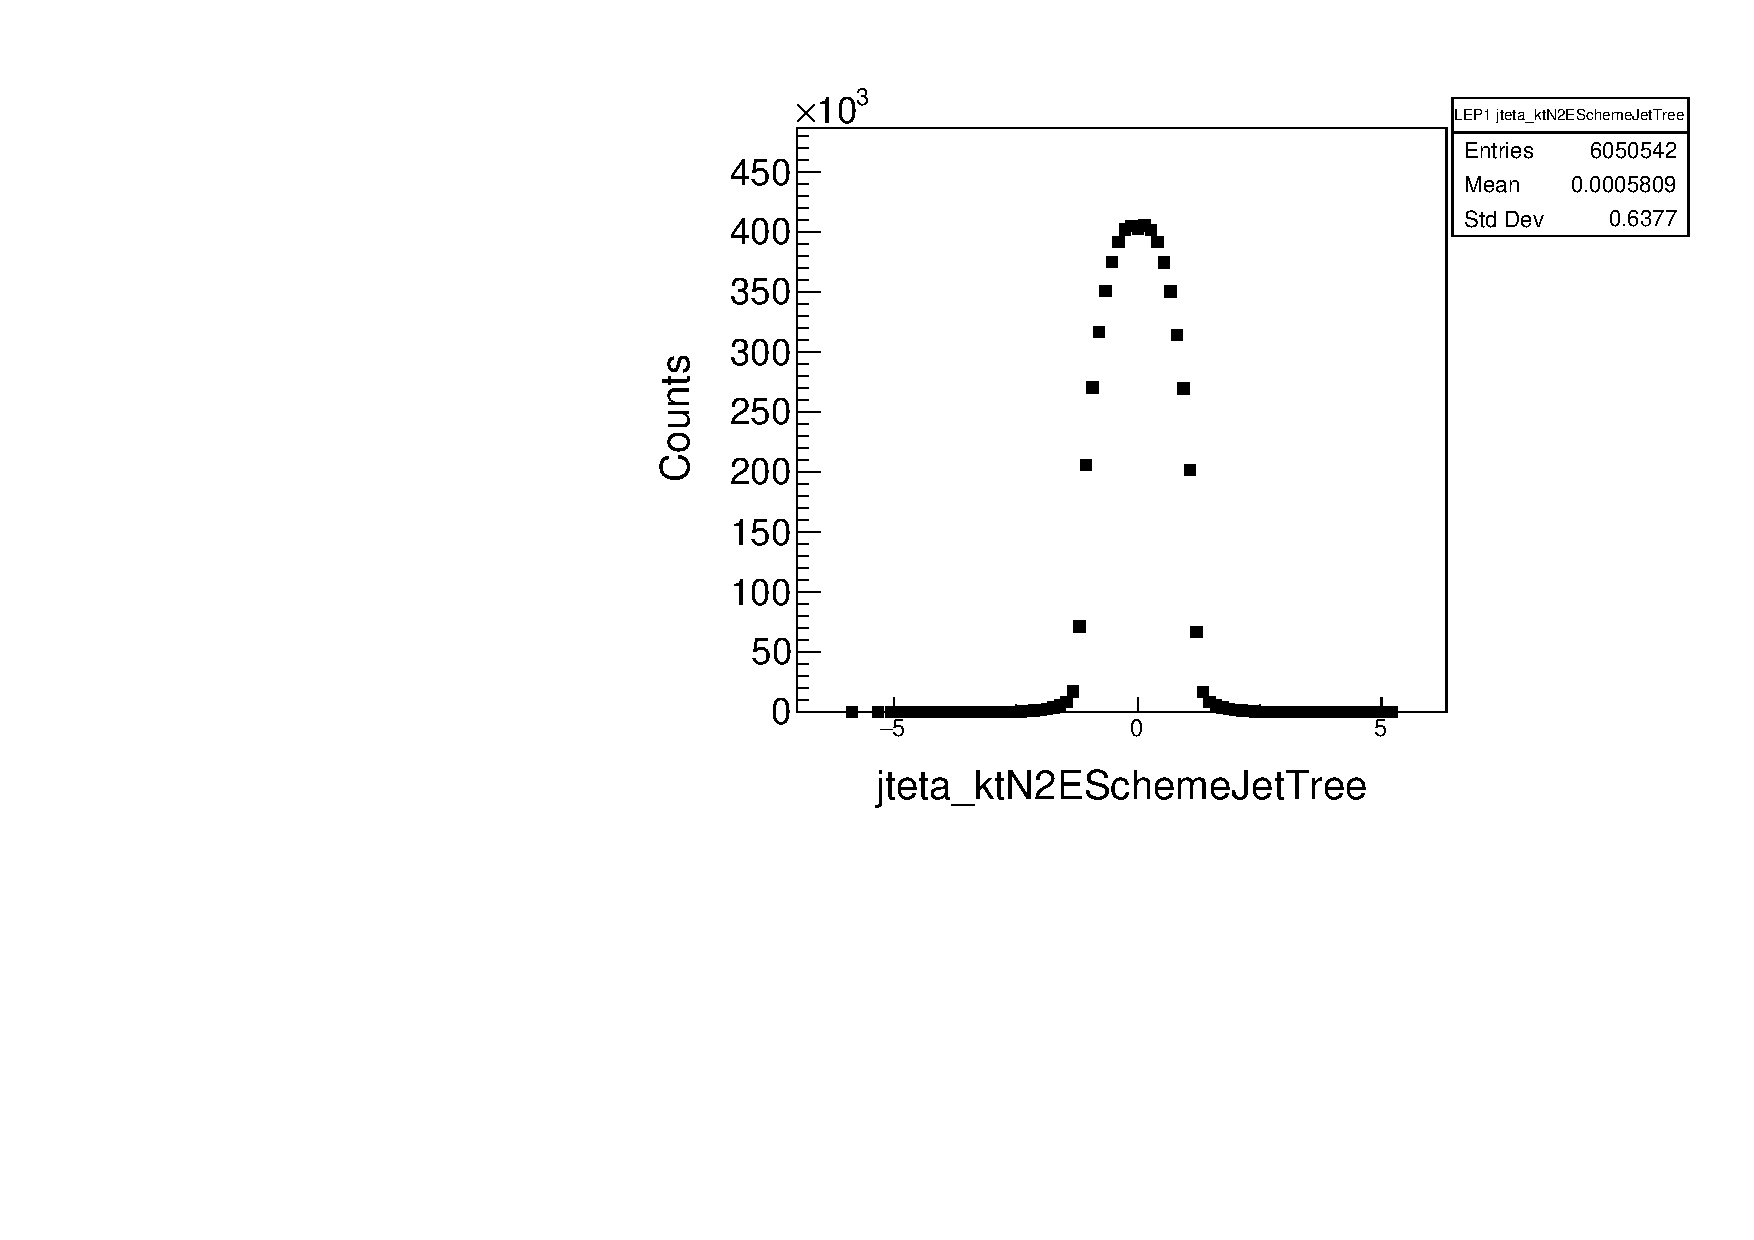
\includegraphics[width=.25\textwidth]{images/DQC/LEP1/jteta_ktN2ESchemeJetTree.pdf}}\hfill
\subfloat{\label{sfig:f}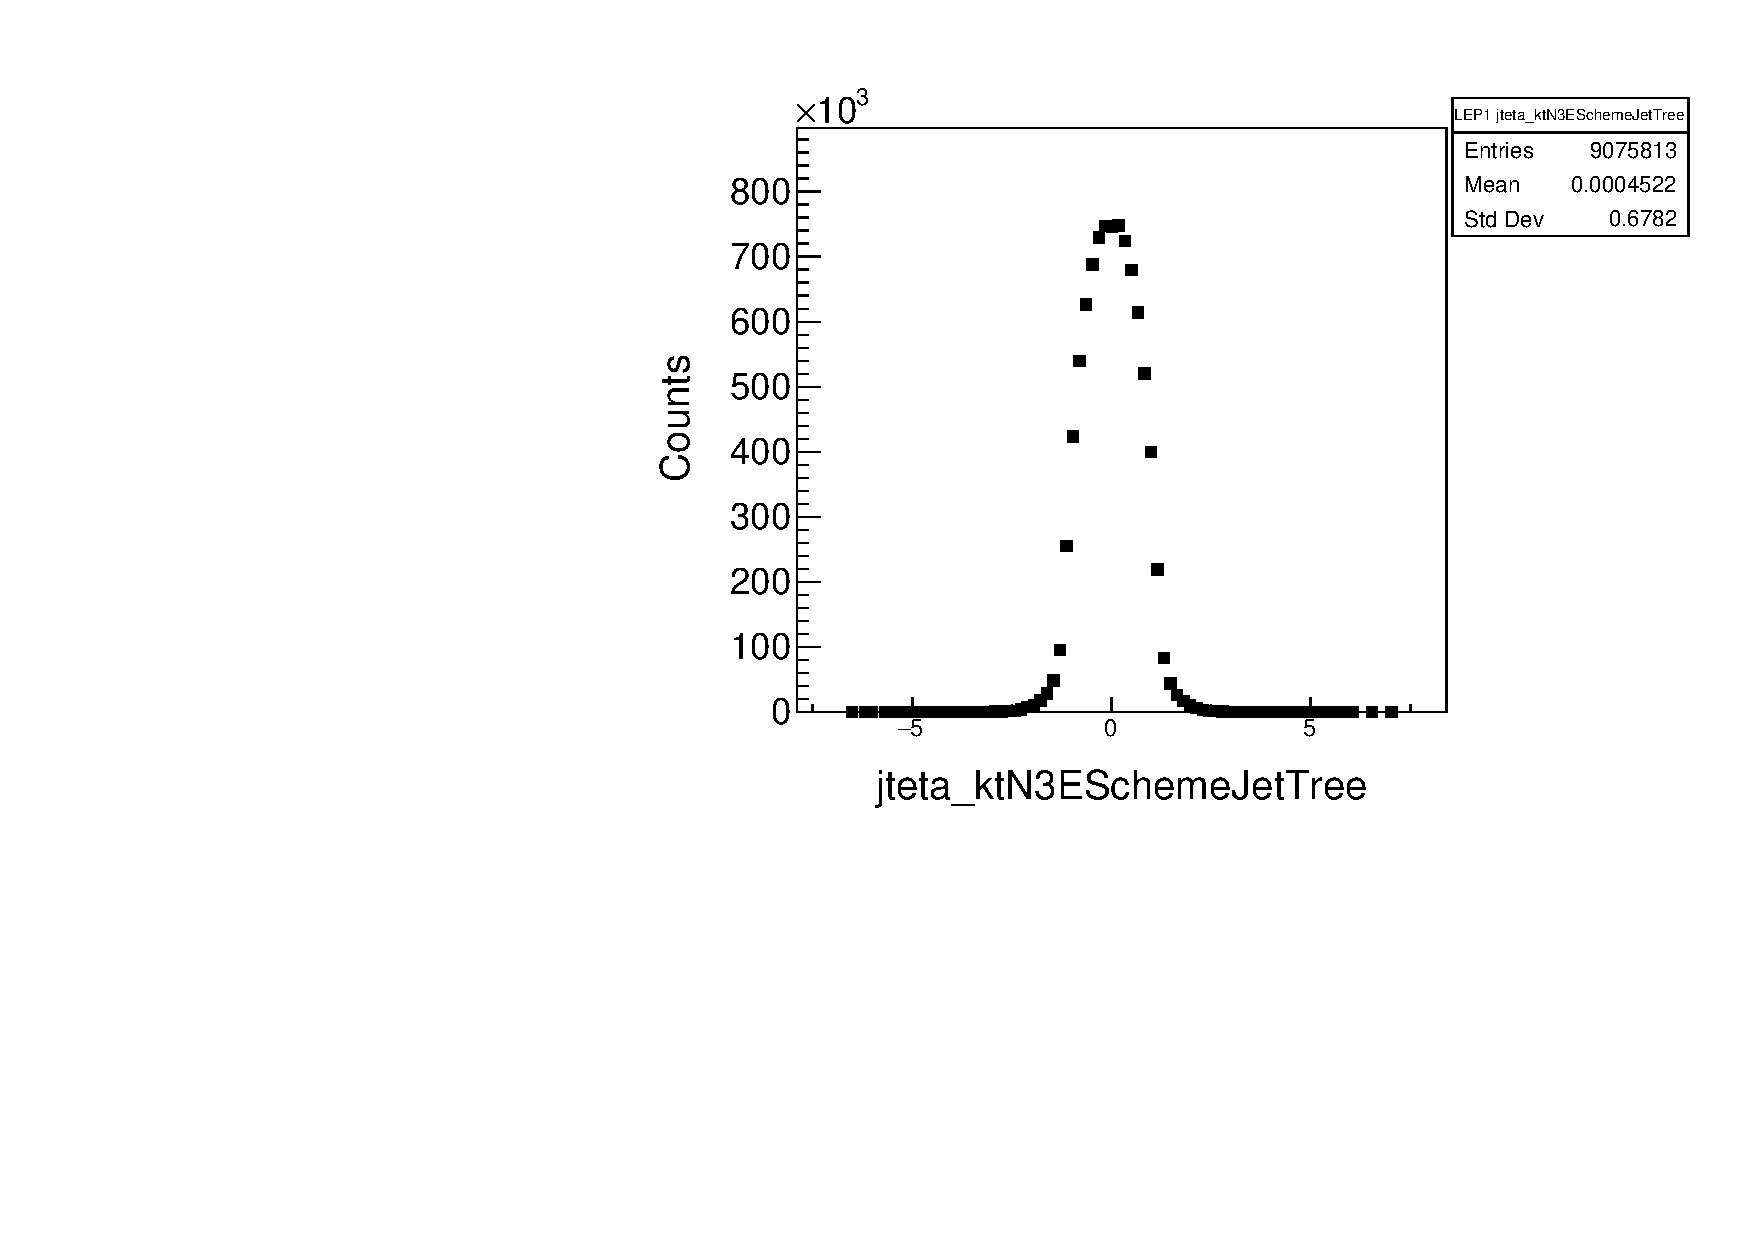
\includegraphics[width=.25\textwidth]{images/DQC/LEP1/jteta_ktN3ESchemeJetTree.pdf}}\hfill
\subfloat{\label{sfig:g}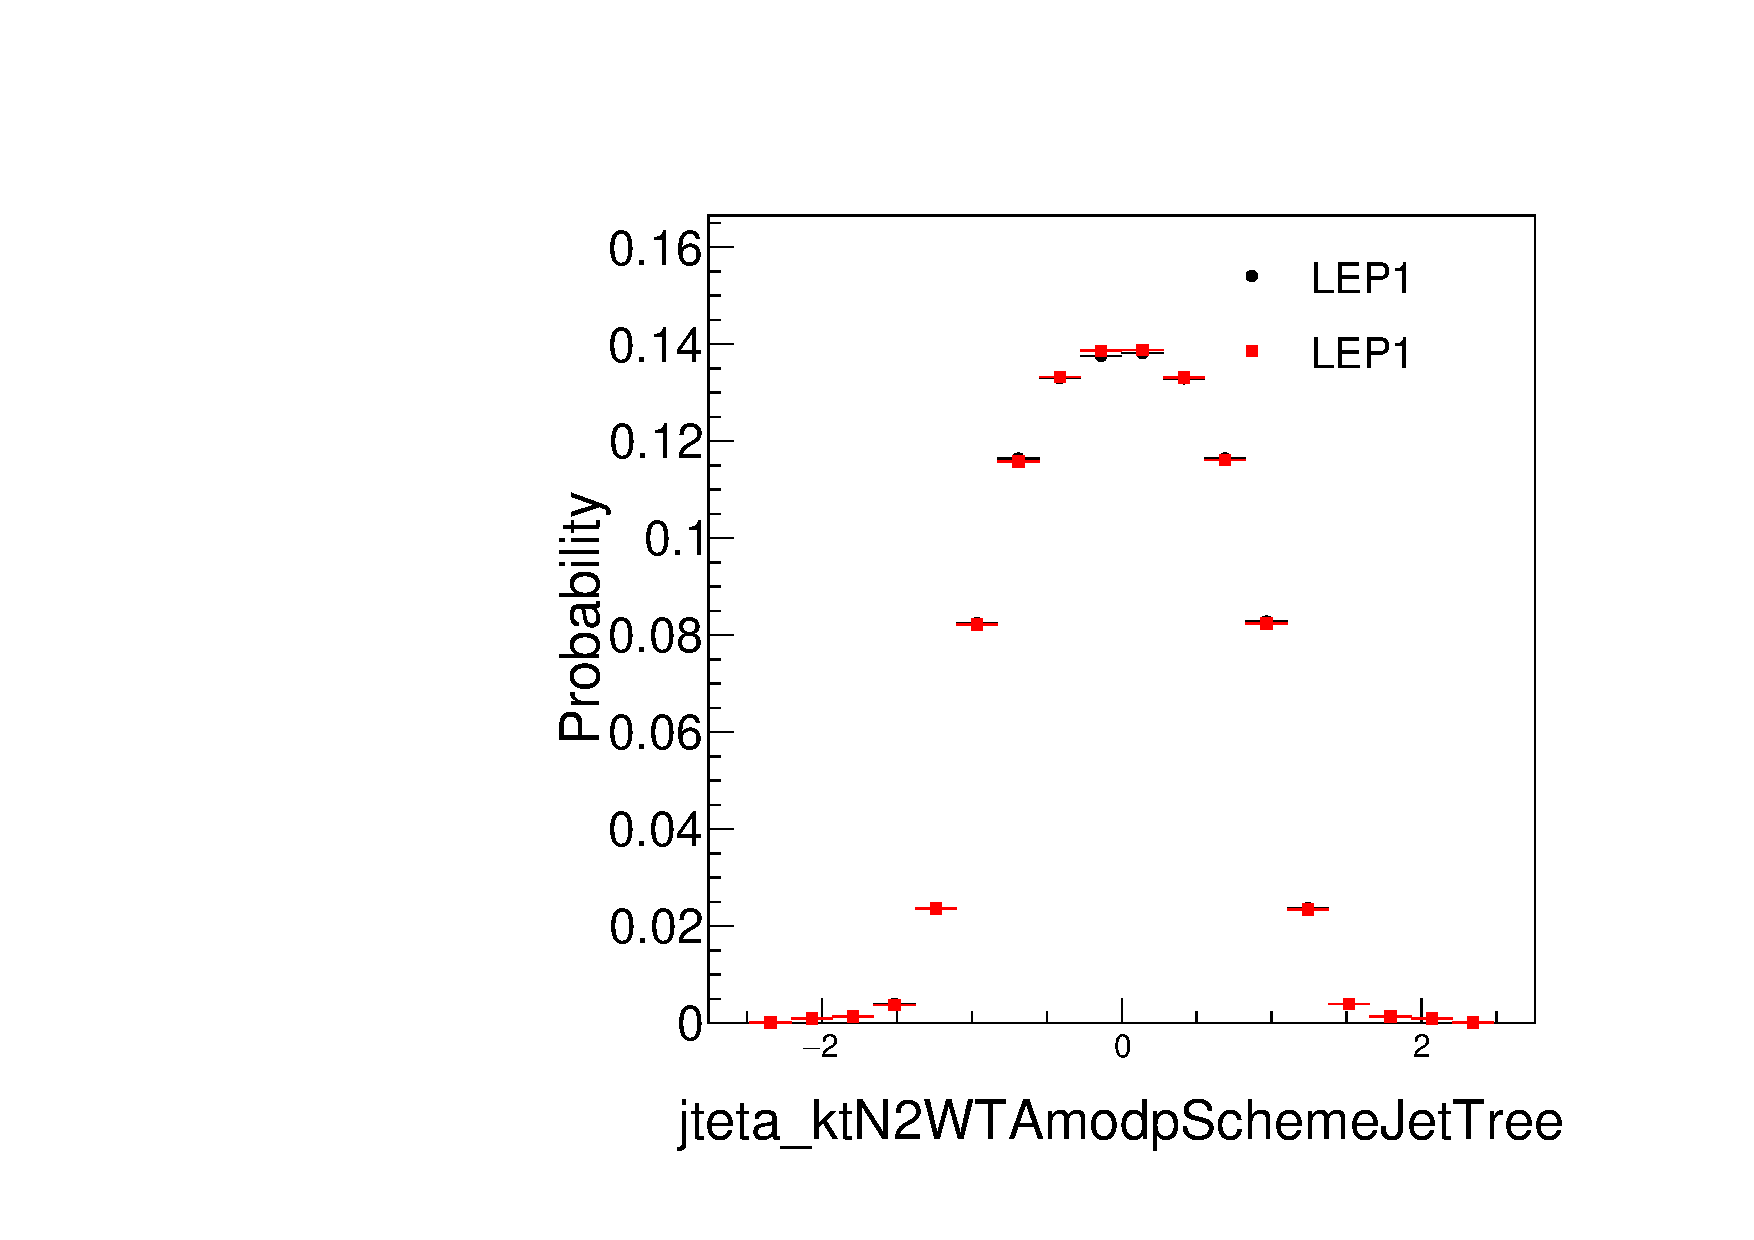
\includegraphics[width=.25\textwidth]{images/DQC/LEP1/jteta_ktN2WTAmodpSchemeJetTree.pdf}}\hfill
\subfloat{\label{sfig:h}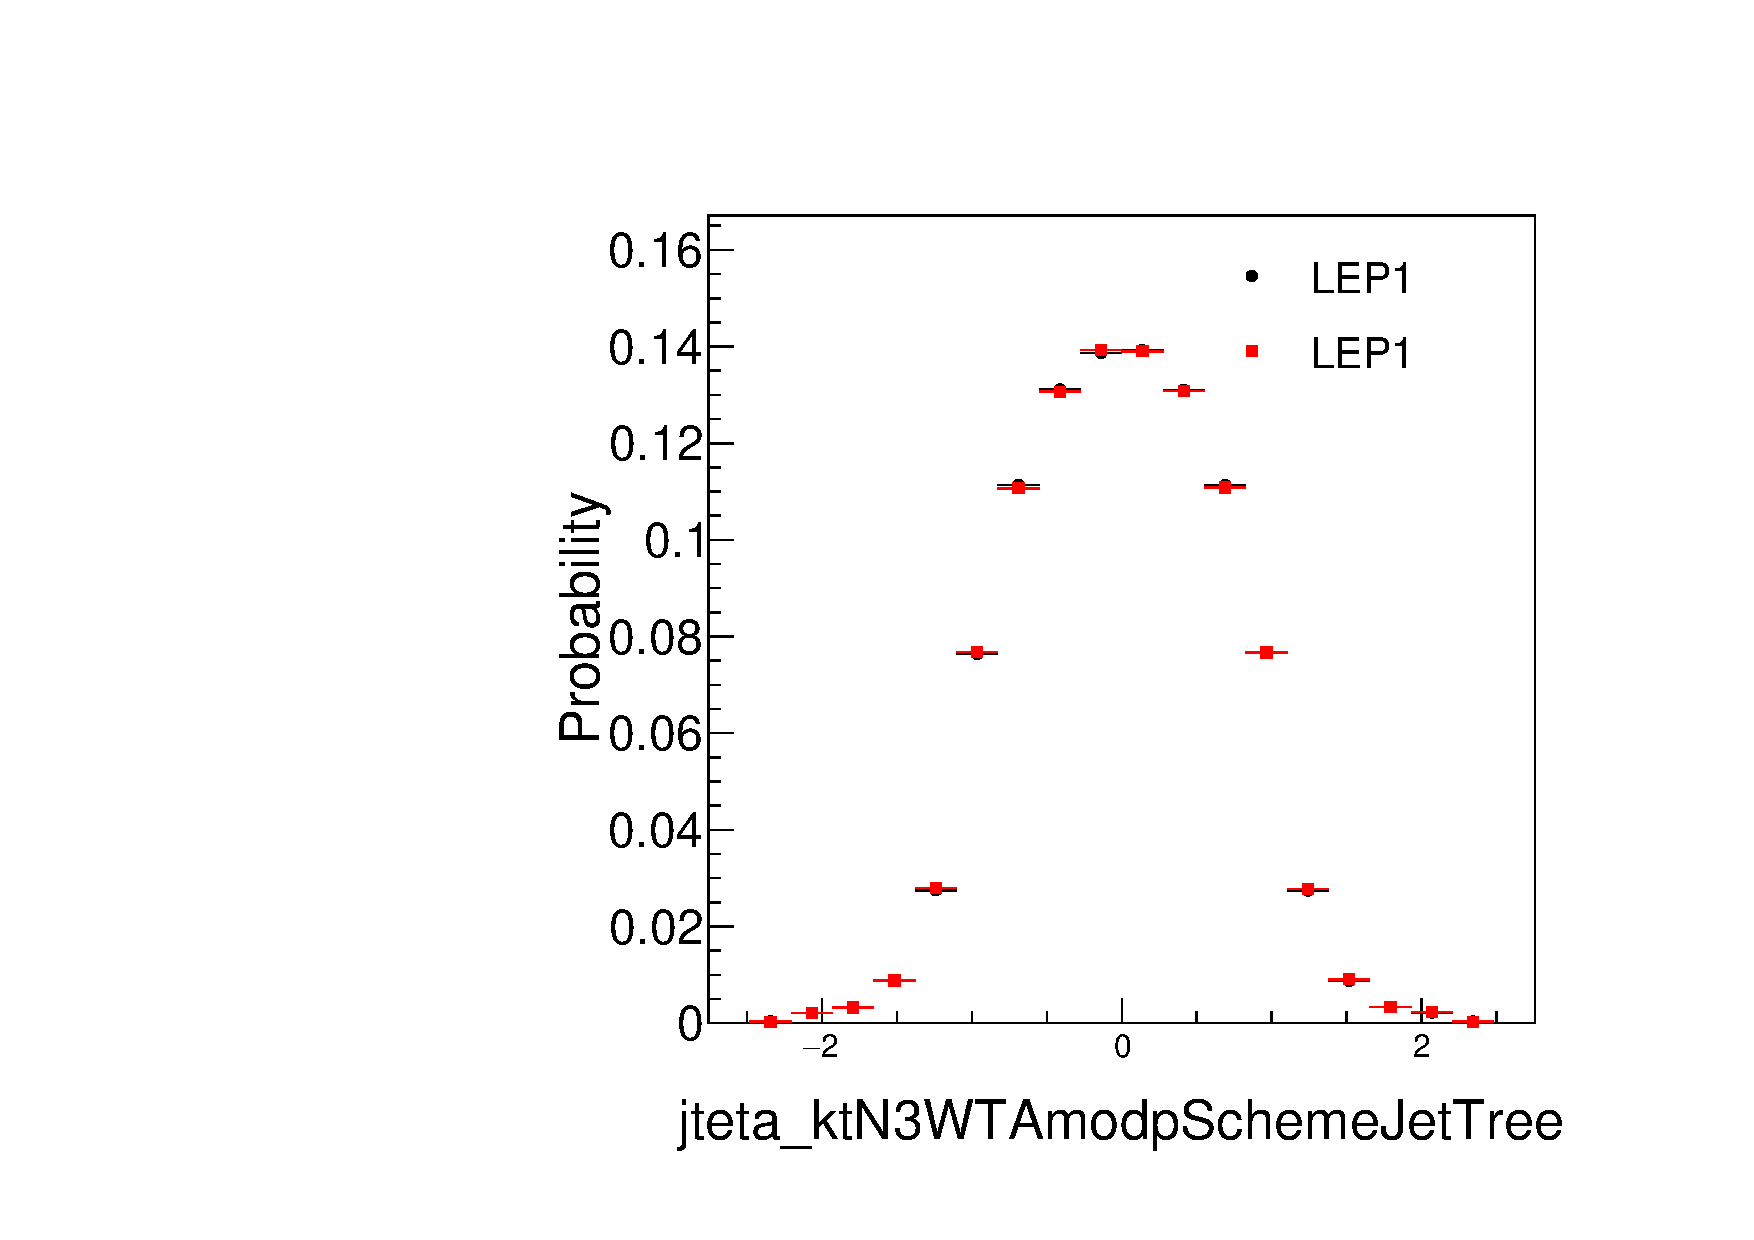
\includegraphics[width=.25\textwidth]{images/DQC/LEP1/jteta_ktN3WTAmodpSchemeJetTree.pdf}}\hfill
\caption{LEP1 Jet $\eta$ distributions. Top row: anti-$k_t$, left to right: $R=0.4$, $E$ scheme; $R=0.8$, $E$ scheme; $R=0.4$, WTA mod p scheme; $R=0.8$, WTA mod p scheme. Bottom row: $k_t$, left to right: $N=2$, $E$ scheme; $N=3$, $E$ scheme; $N=2$, WTA mod p scheme; $N=3$; WTA mod p scheme.}  
\end{figure}

\begin{figure}[H]
\centering
\subfloat{\label{sfig:a}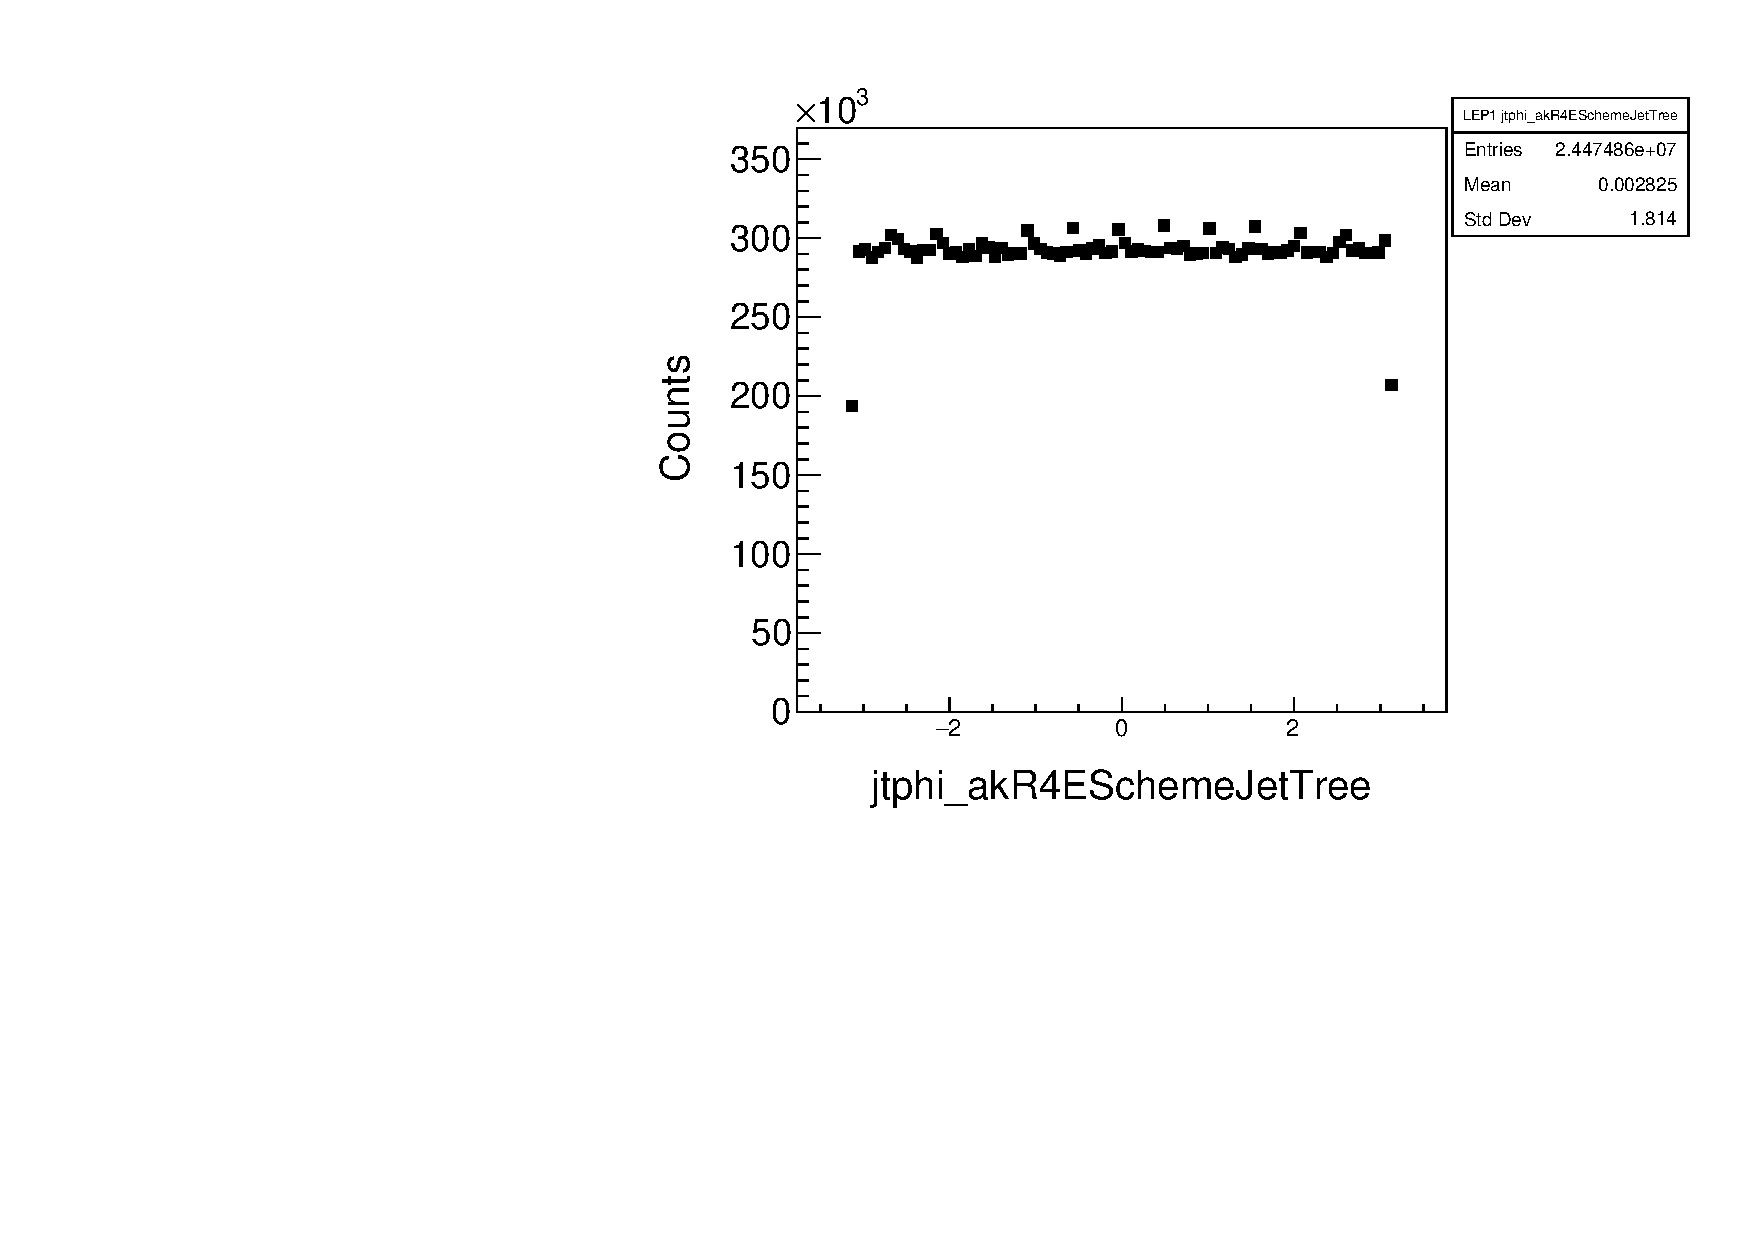
\includegraphics[width=.25\textwidth]{images/DQC/LEP1/jtphi_akR4ESchemeJetTree.pdf}}\hfill
\subfloat{\label{sfig:b}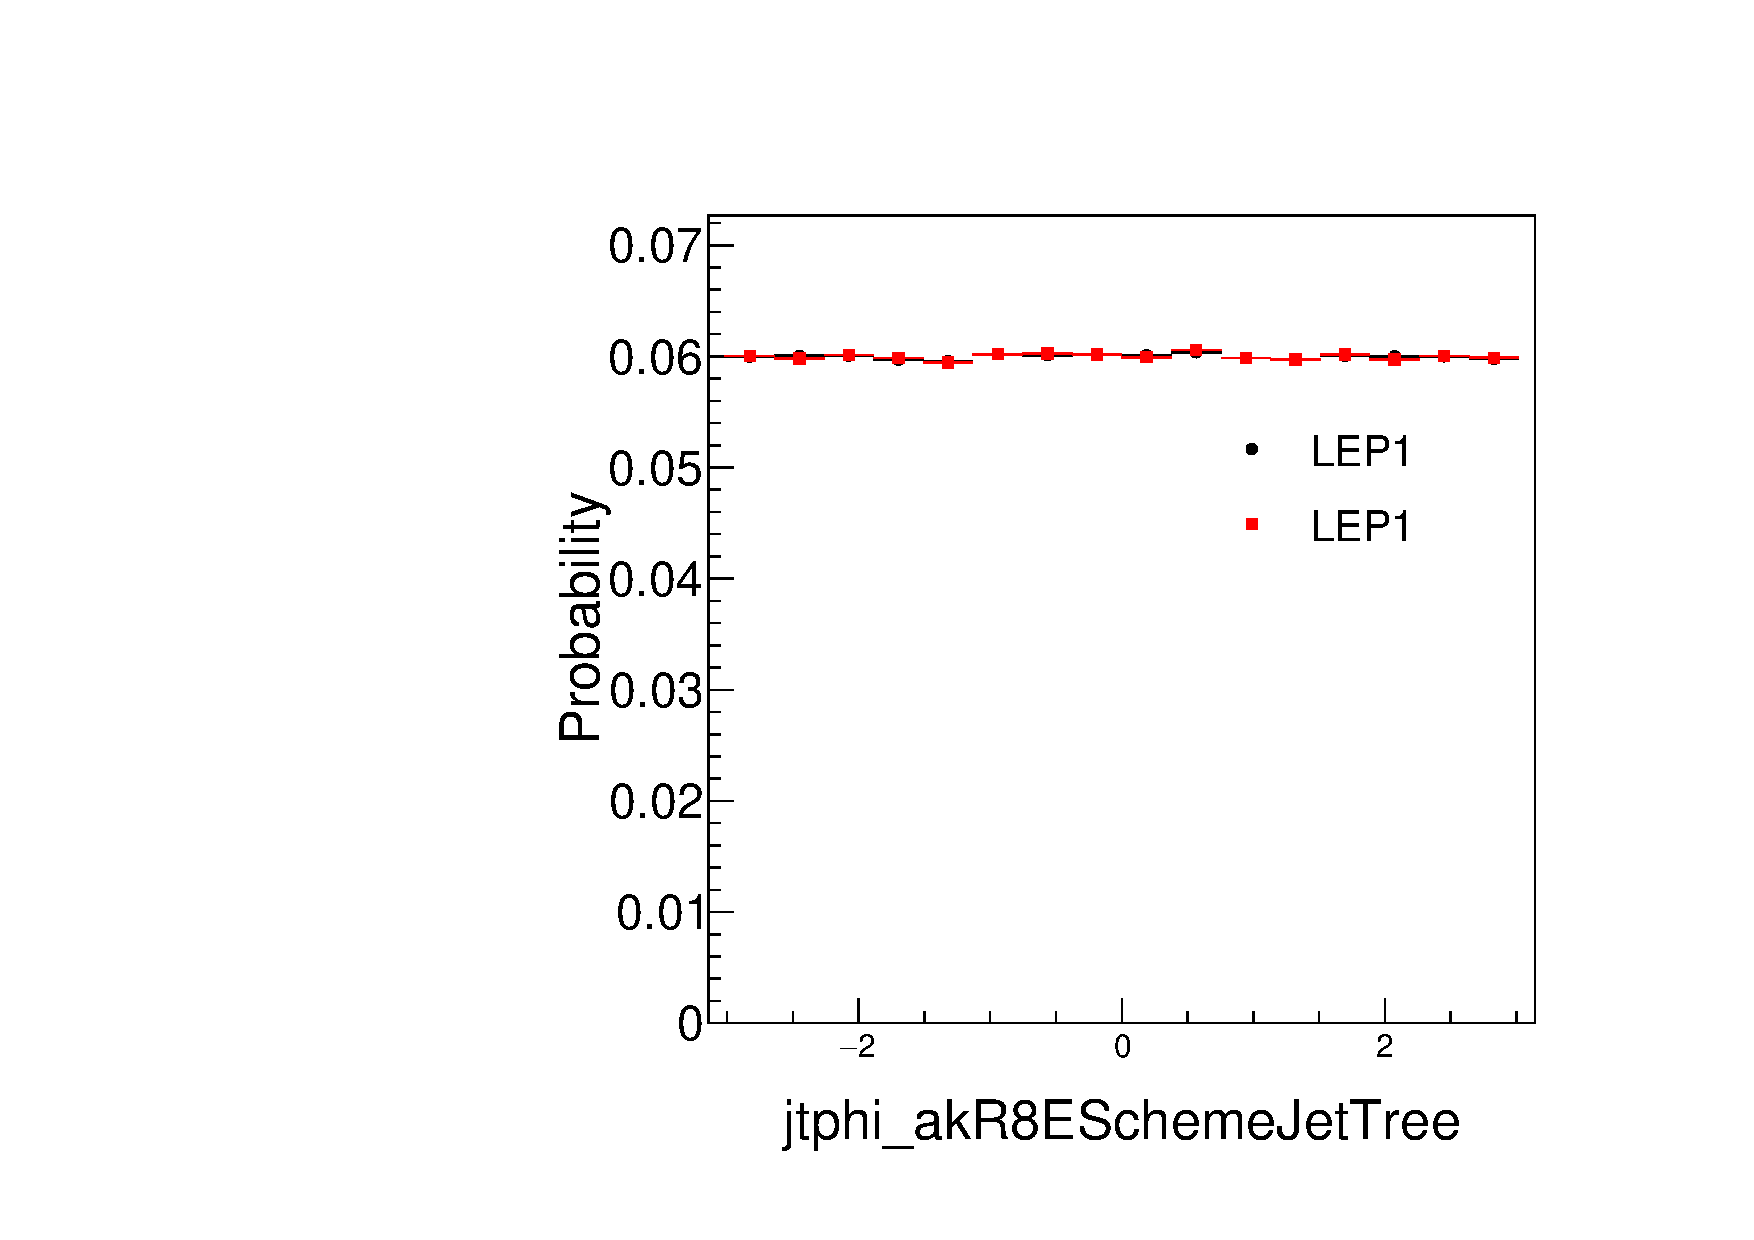
\includegraphics[width=.25\textwidth]{images/DQC/LEP1/jtphi_akR8ESchemeJetTree.pdf}}\hfill
\subfloat{\label{sfig:c}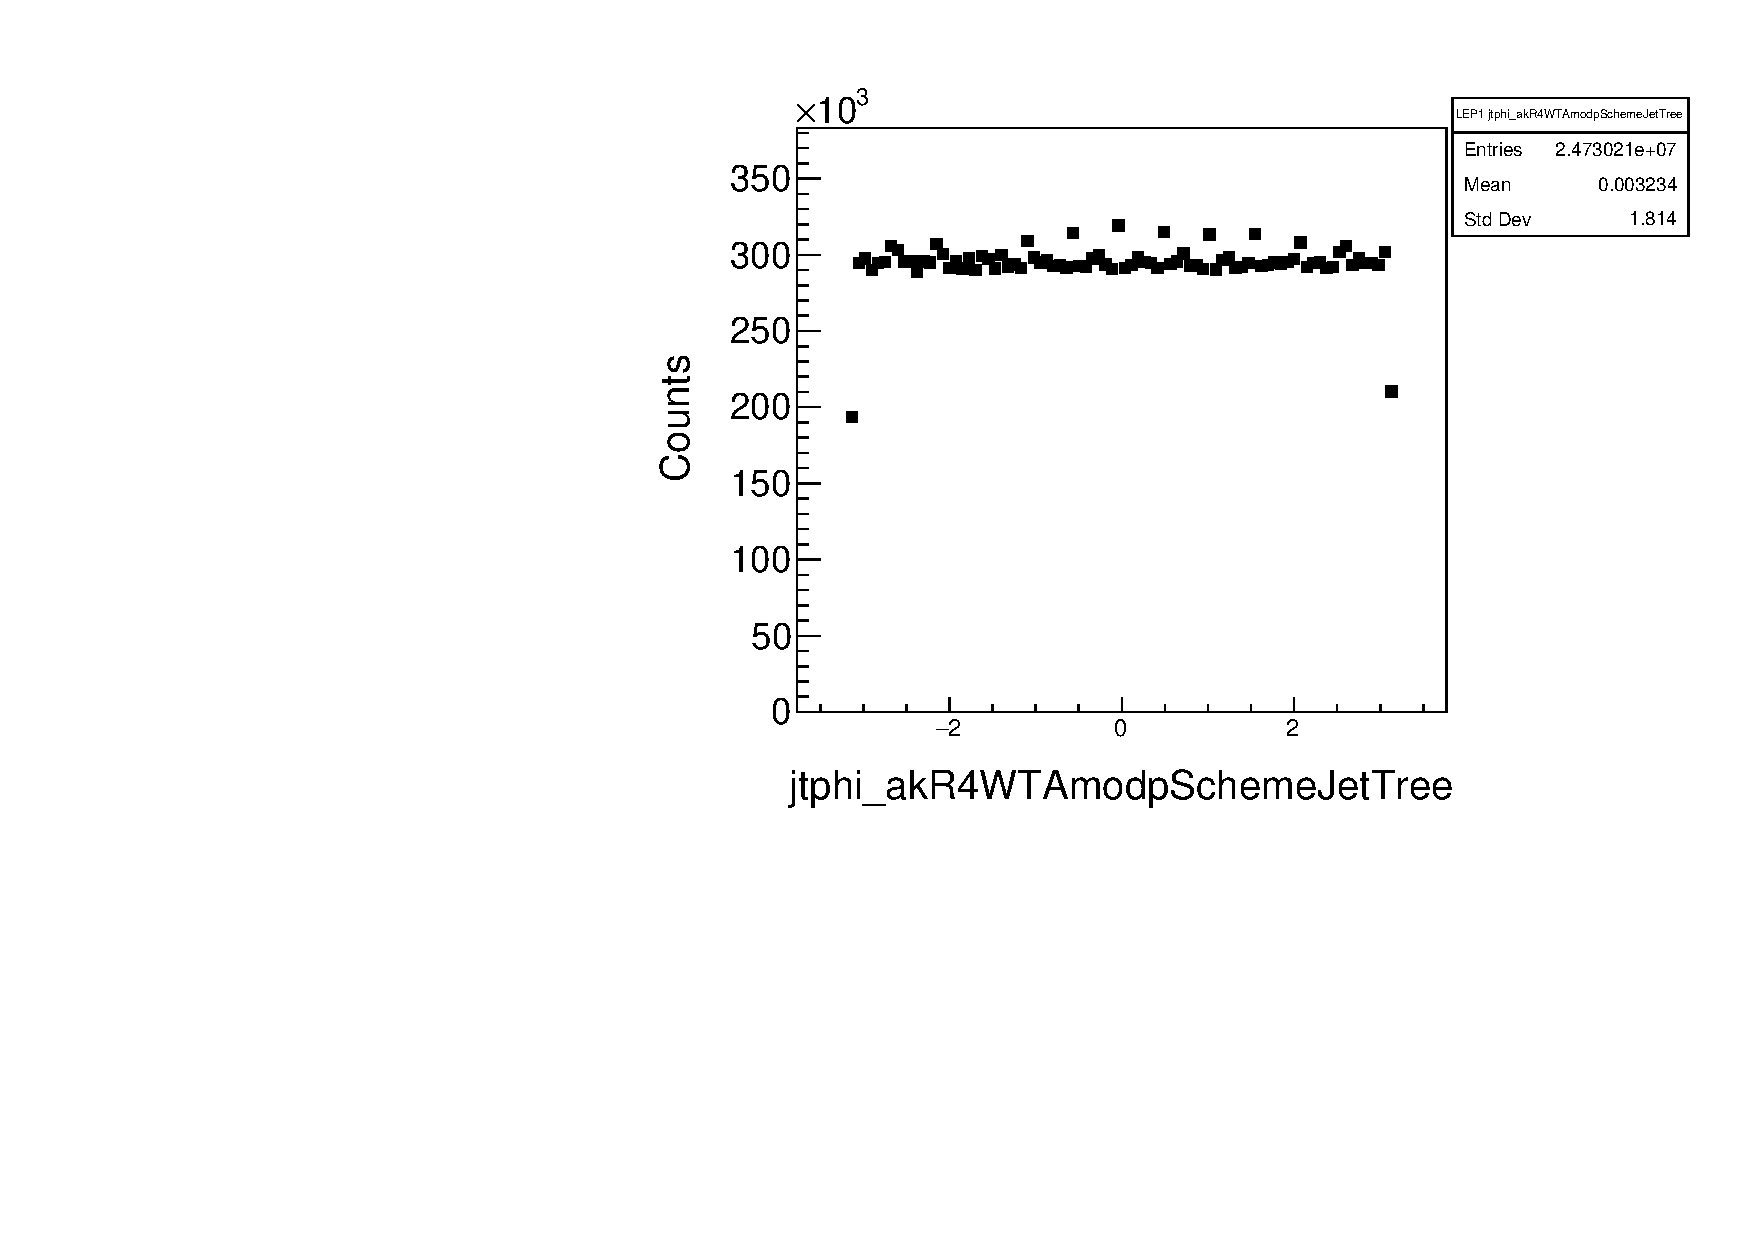
\includegraphics[width=.25\textwidth]{images/DQC/LEP1/jtphi_akR4WTAmodpSchemeJetTree.pdf}}\hfill
\subfloat{\label{sfig:d}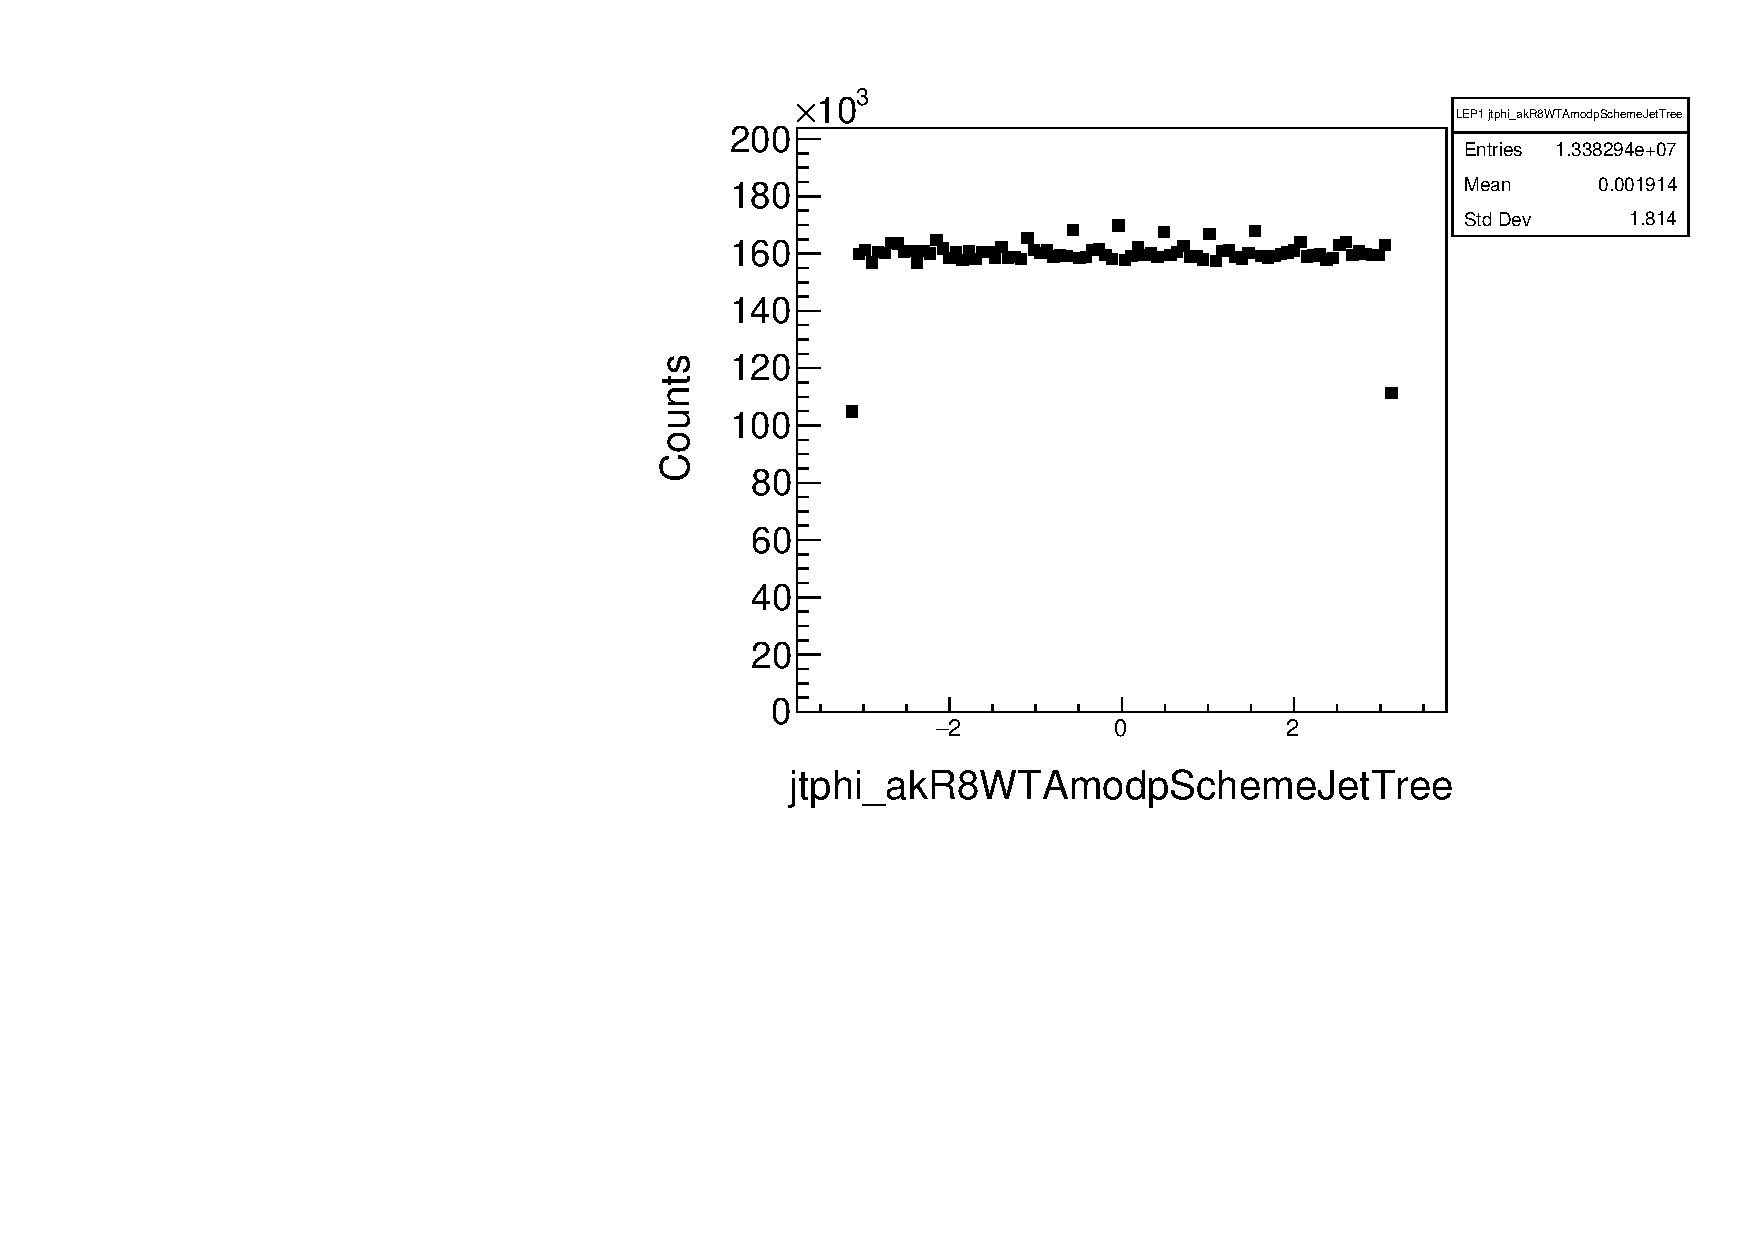
\includegraphics[width=.25\textwidth]{images/DQC/LEP1/jtphi_akR8WTAmodpSchemeJetTree.pdf}}\hfill %row end
\subfloat{\label{sfig:e}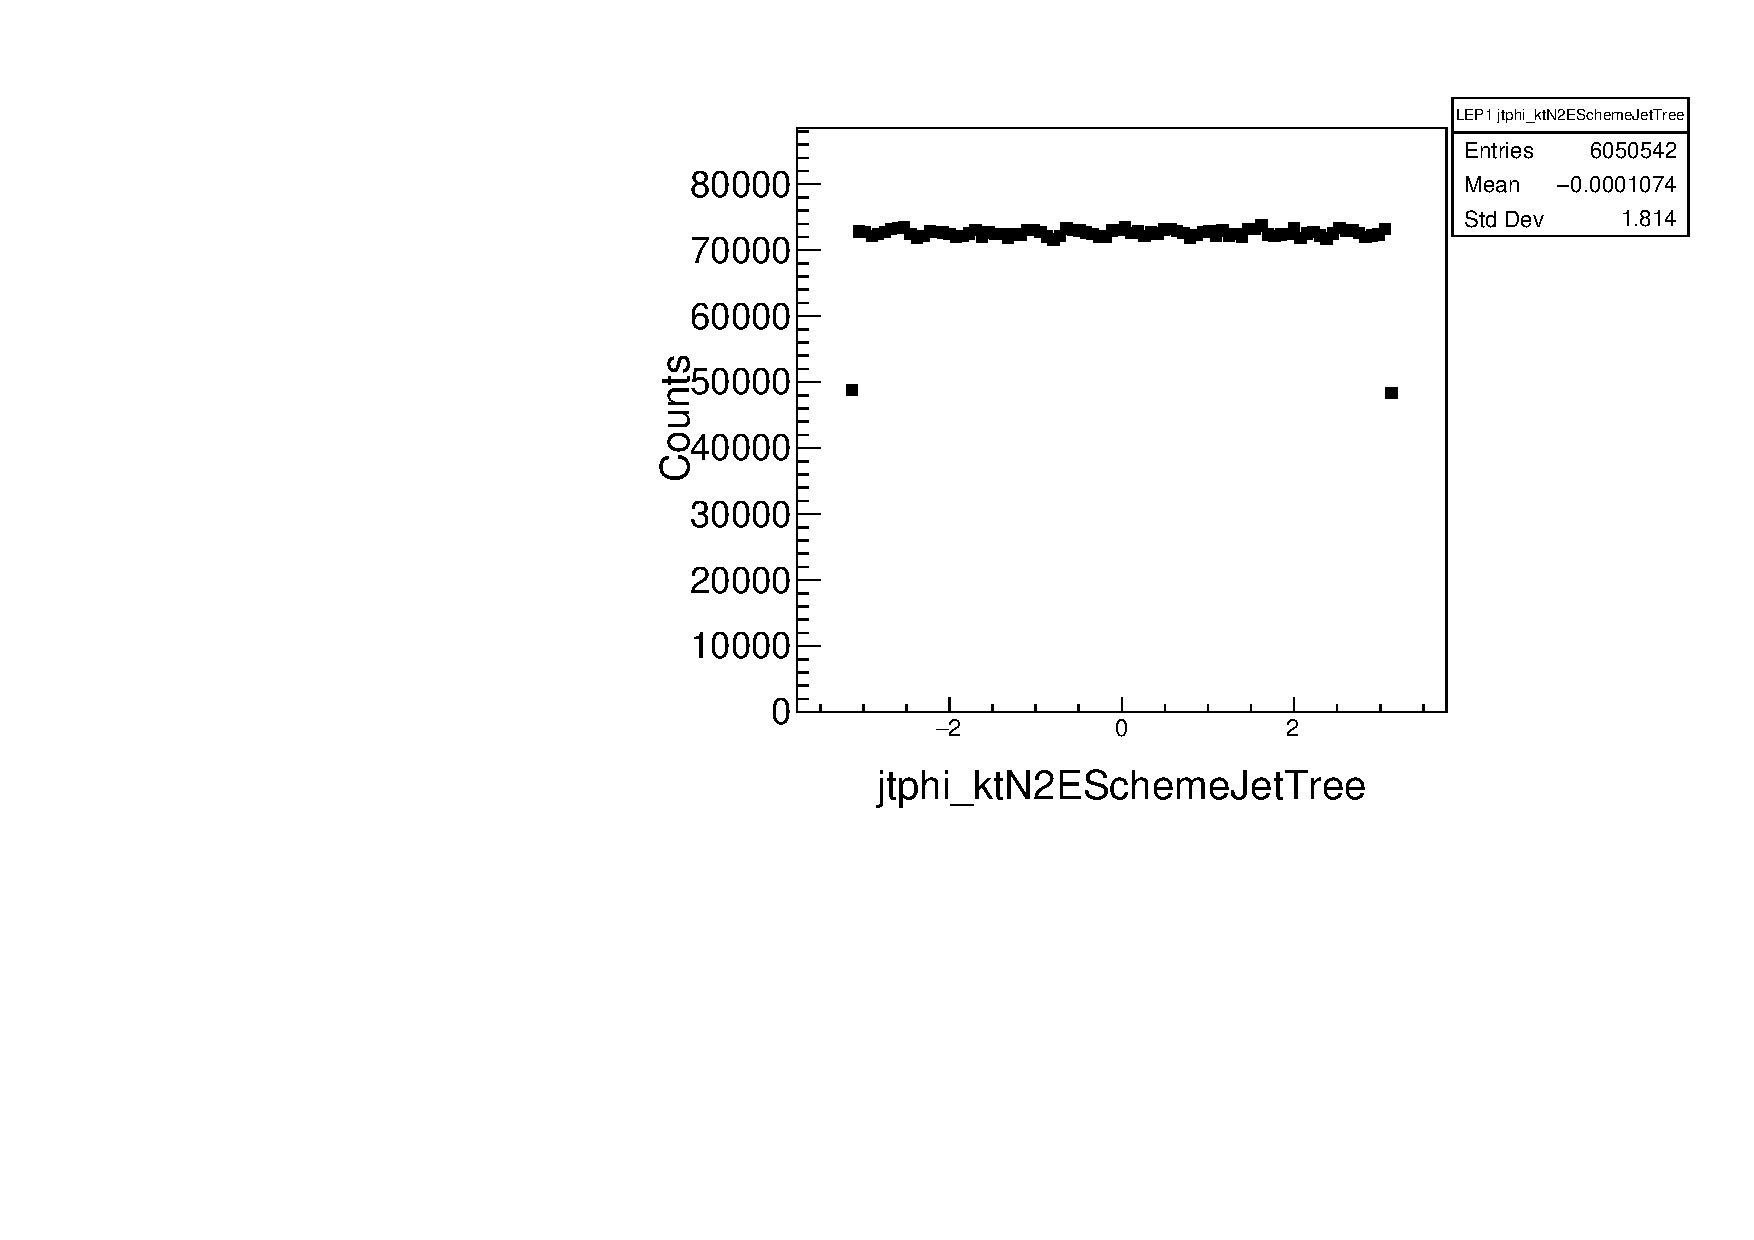
\includegraphics[width=.25\textwidth]{images/DQC/LEP1/jtphi_ktN2ESchemeJetTree.pdf}}\hfill
\subfloat{\label{sfig:f}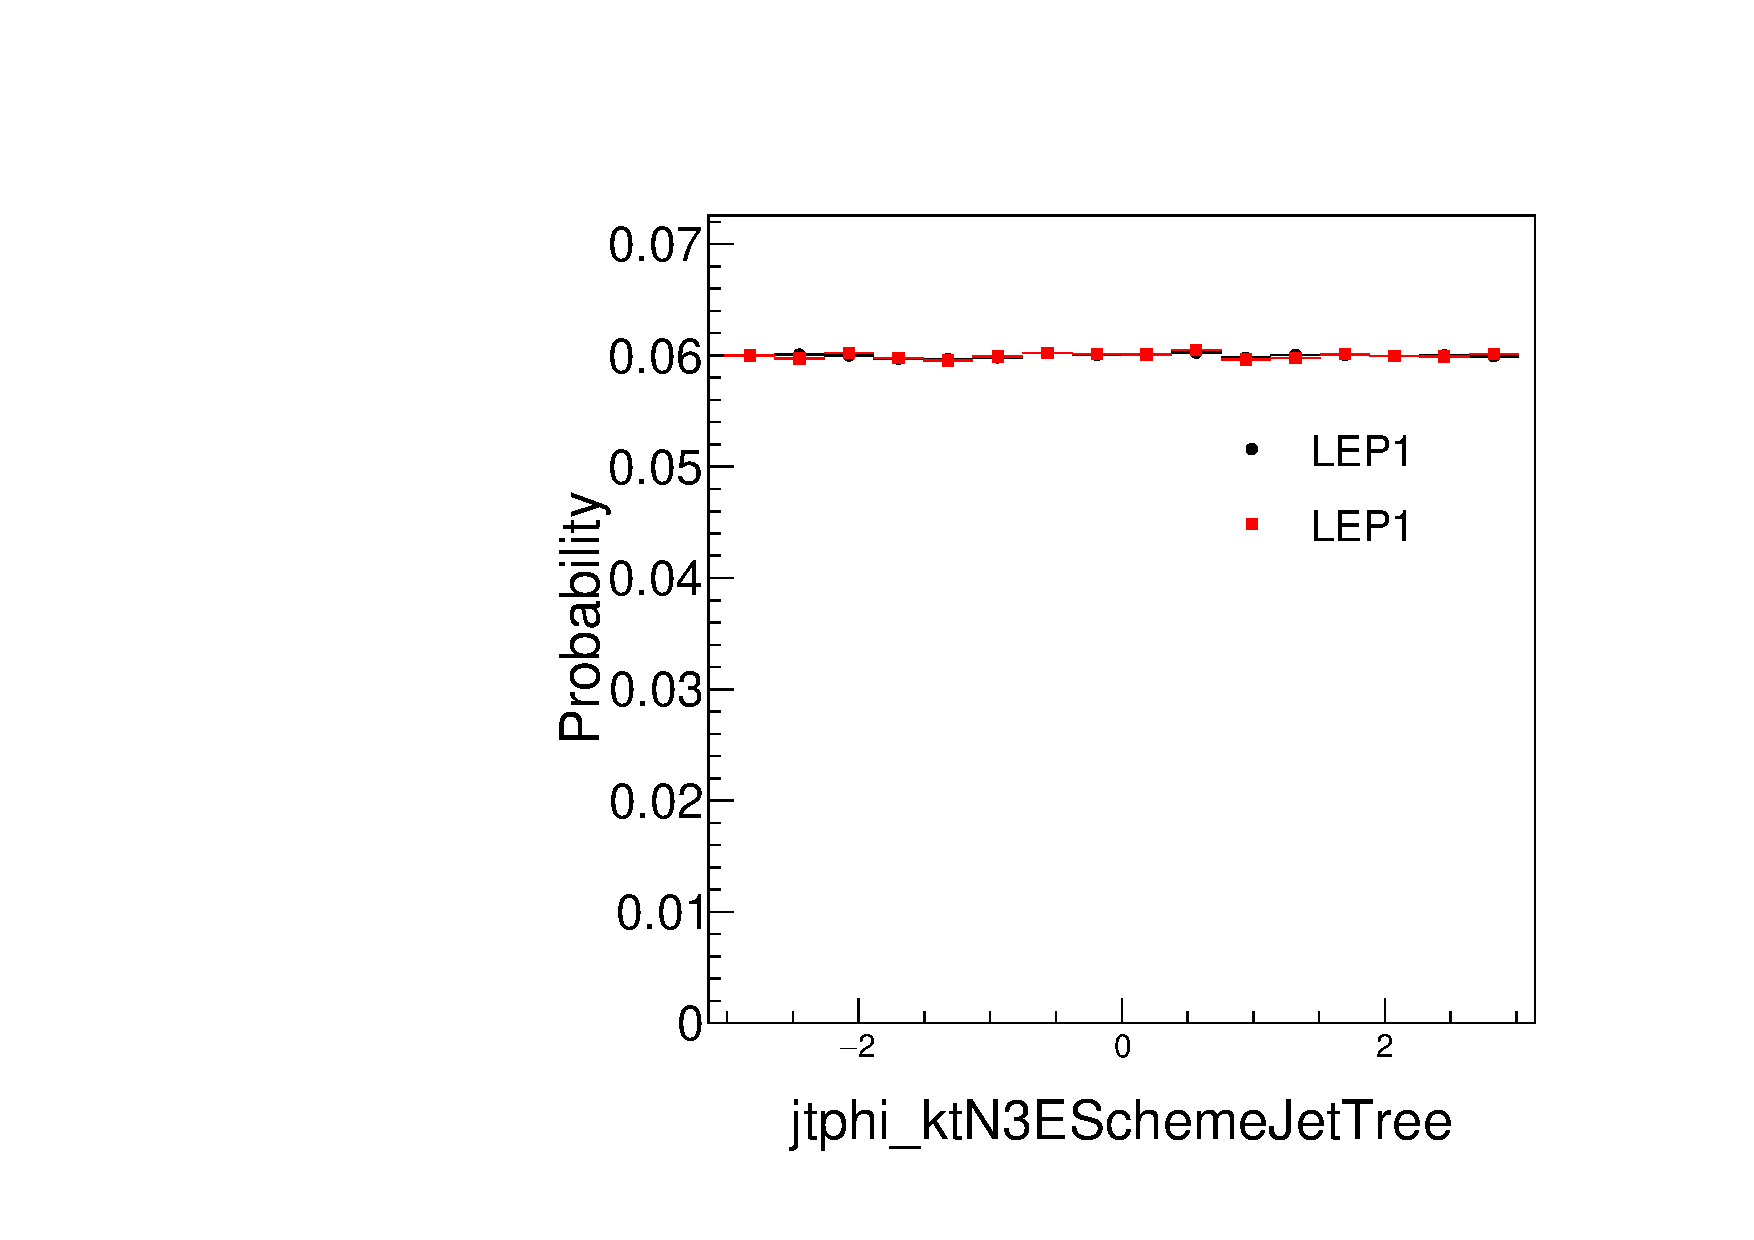
\includegraphics[width=.25\textwidth]{images/DQC/LEP1/jtphi_ktN3ESchemeJetTree.pdf}}\hfill
\subfloat{\label{sfig:g}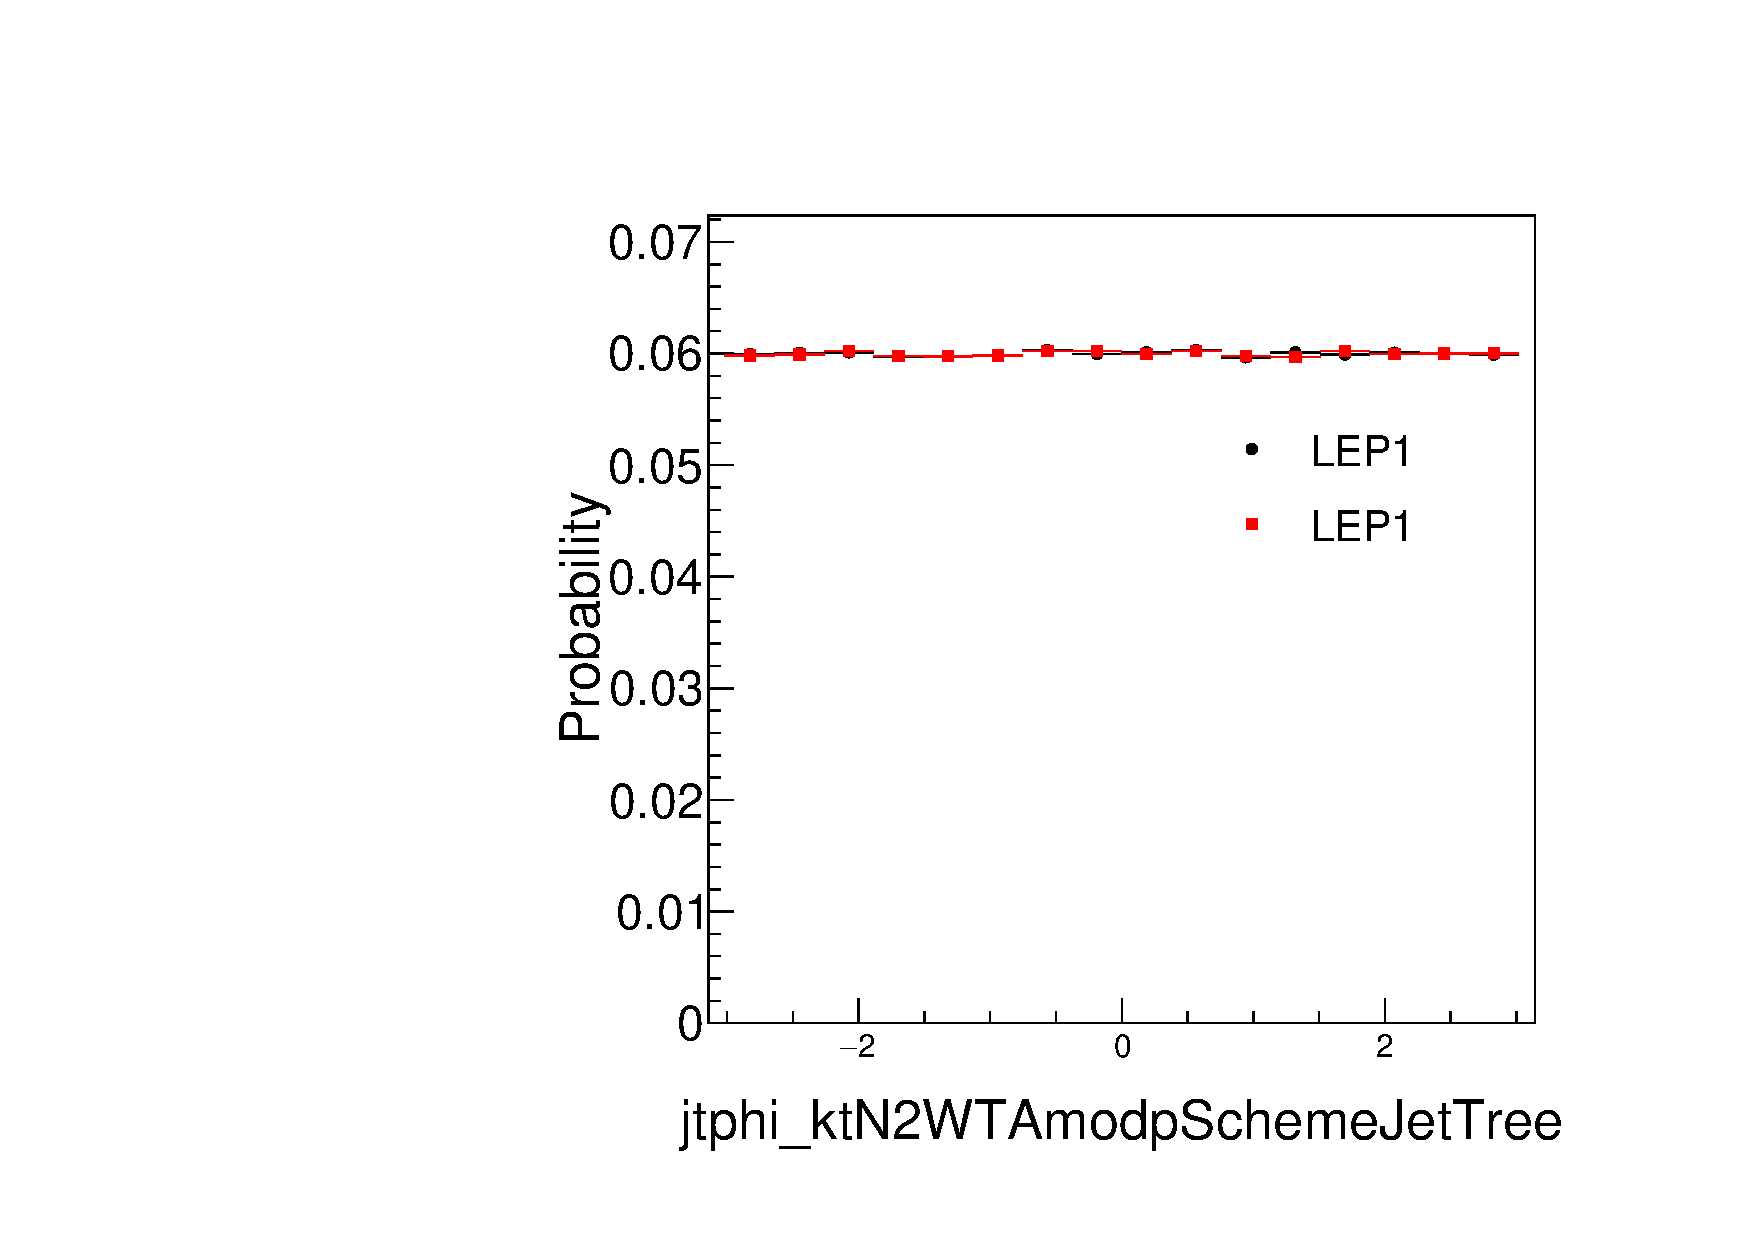
\includegraphics[width=.25\textwidth]{images/DQC/LEP1/jtphi_ktN2WTAmodpSchemeJetTree.pdf}}\hfill
\subfloat{\label{sfig:h}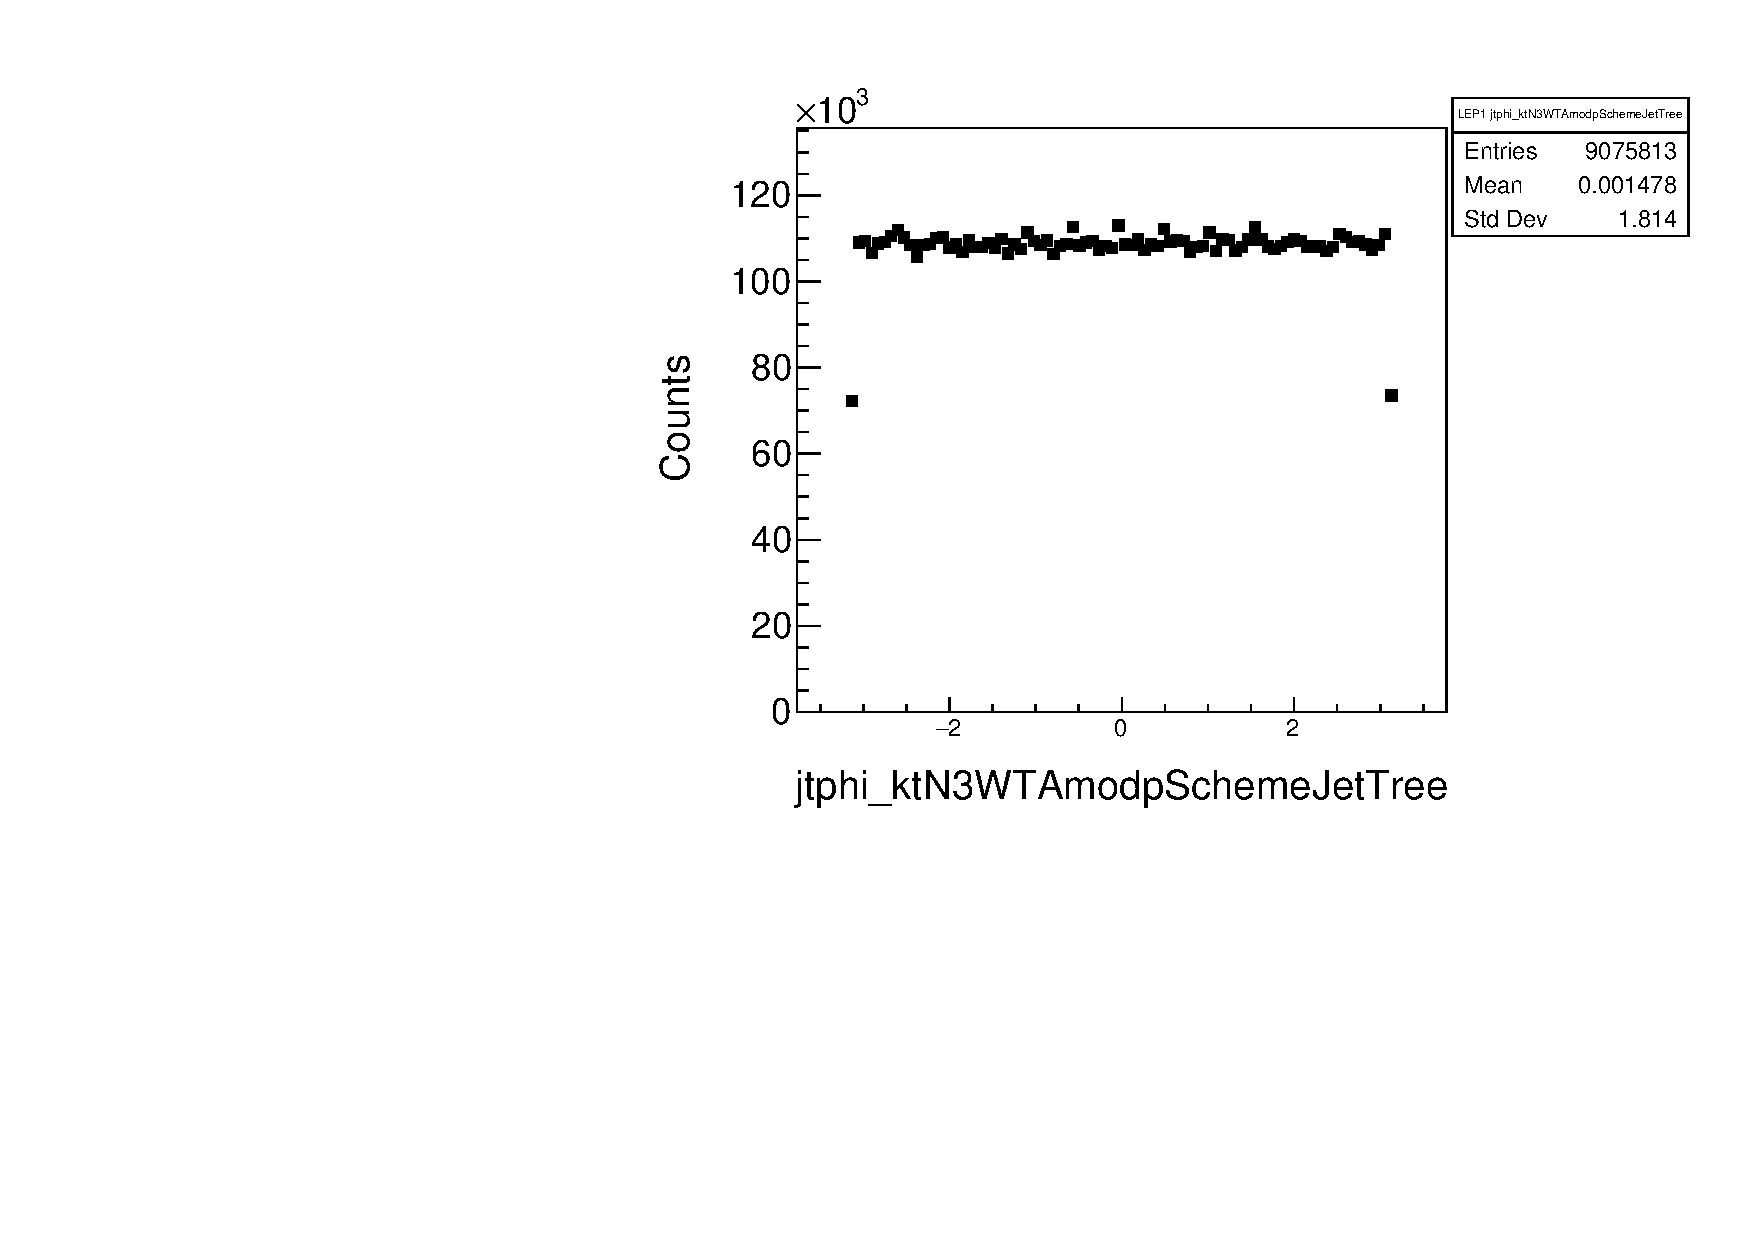
\includegraphics[width=.25\textwidth]{images/DQC/LEP1/jtphi_ktN3WTAmodpSchemeJetTree.pdf}}\hfill
\caption{LEP1 Jet $\phi$ distributions. Top row: anti-$k_t$, left to right: $R=0.4$, $E$ scheme; $R=0.8$, $E$ scheme; $R=0.4$, WTA mod p scheme; $R=0.8$, WTA mod p scheme. Bottom row: $k_t$, left to right: $N=2$, $E$ scheme; $N=3$, $E$ scheme; $N=2$, WTA mod p scheme; $N=3$; WTA mod p scheme.}  
\end{figure}

\begin{figure}[H]
\centering
\subfloat{\label{sfig:a}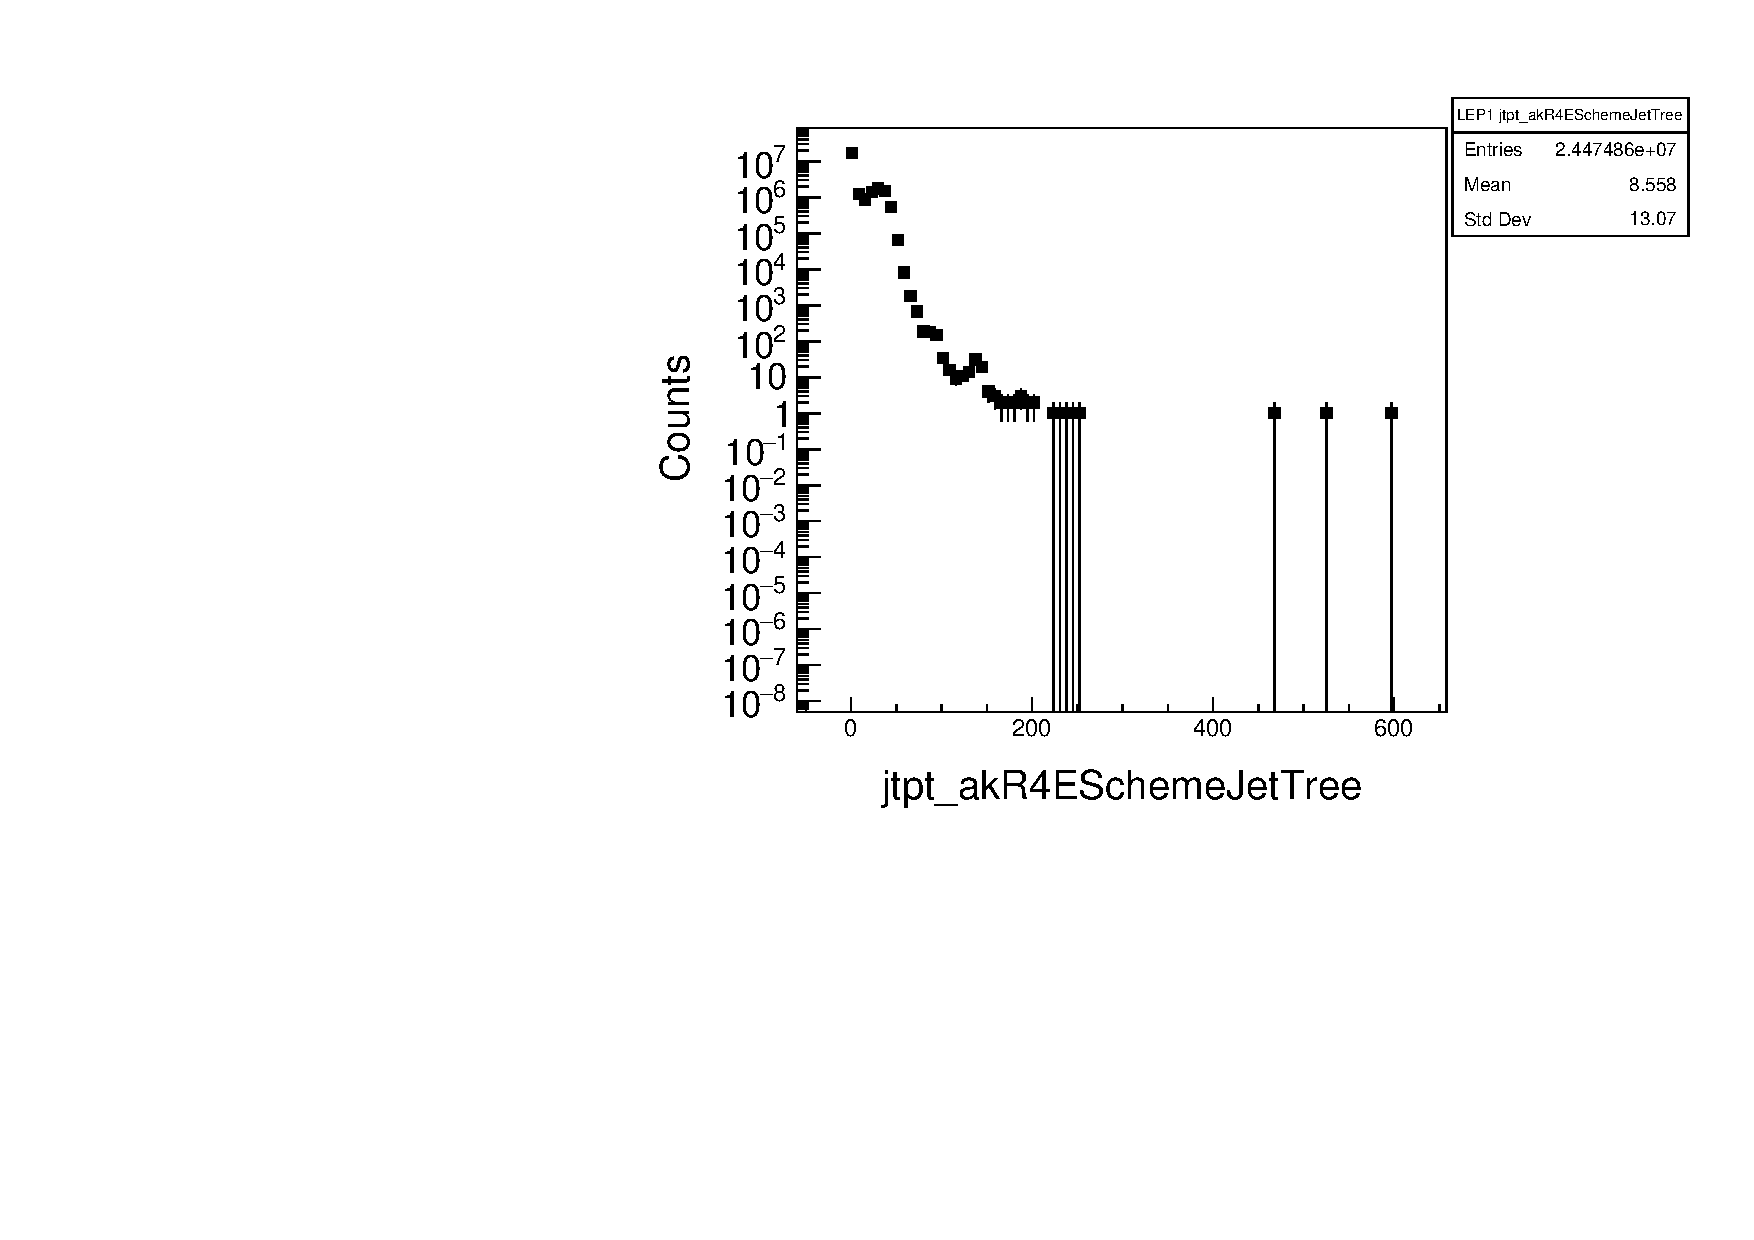
\includegraphics[width=.25\textwidth]{images/DQC/LEP1/jtpt_akR4ESchemeJetTree.pdf}}\hfill
\subfloat{\label{sfig:b}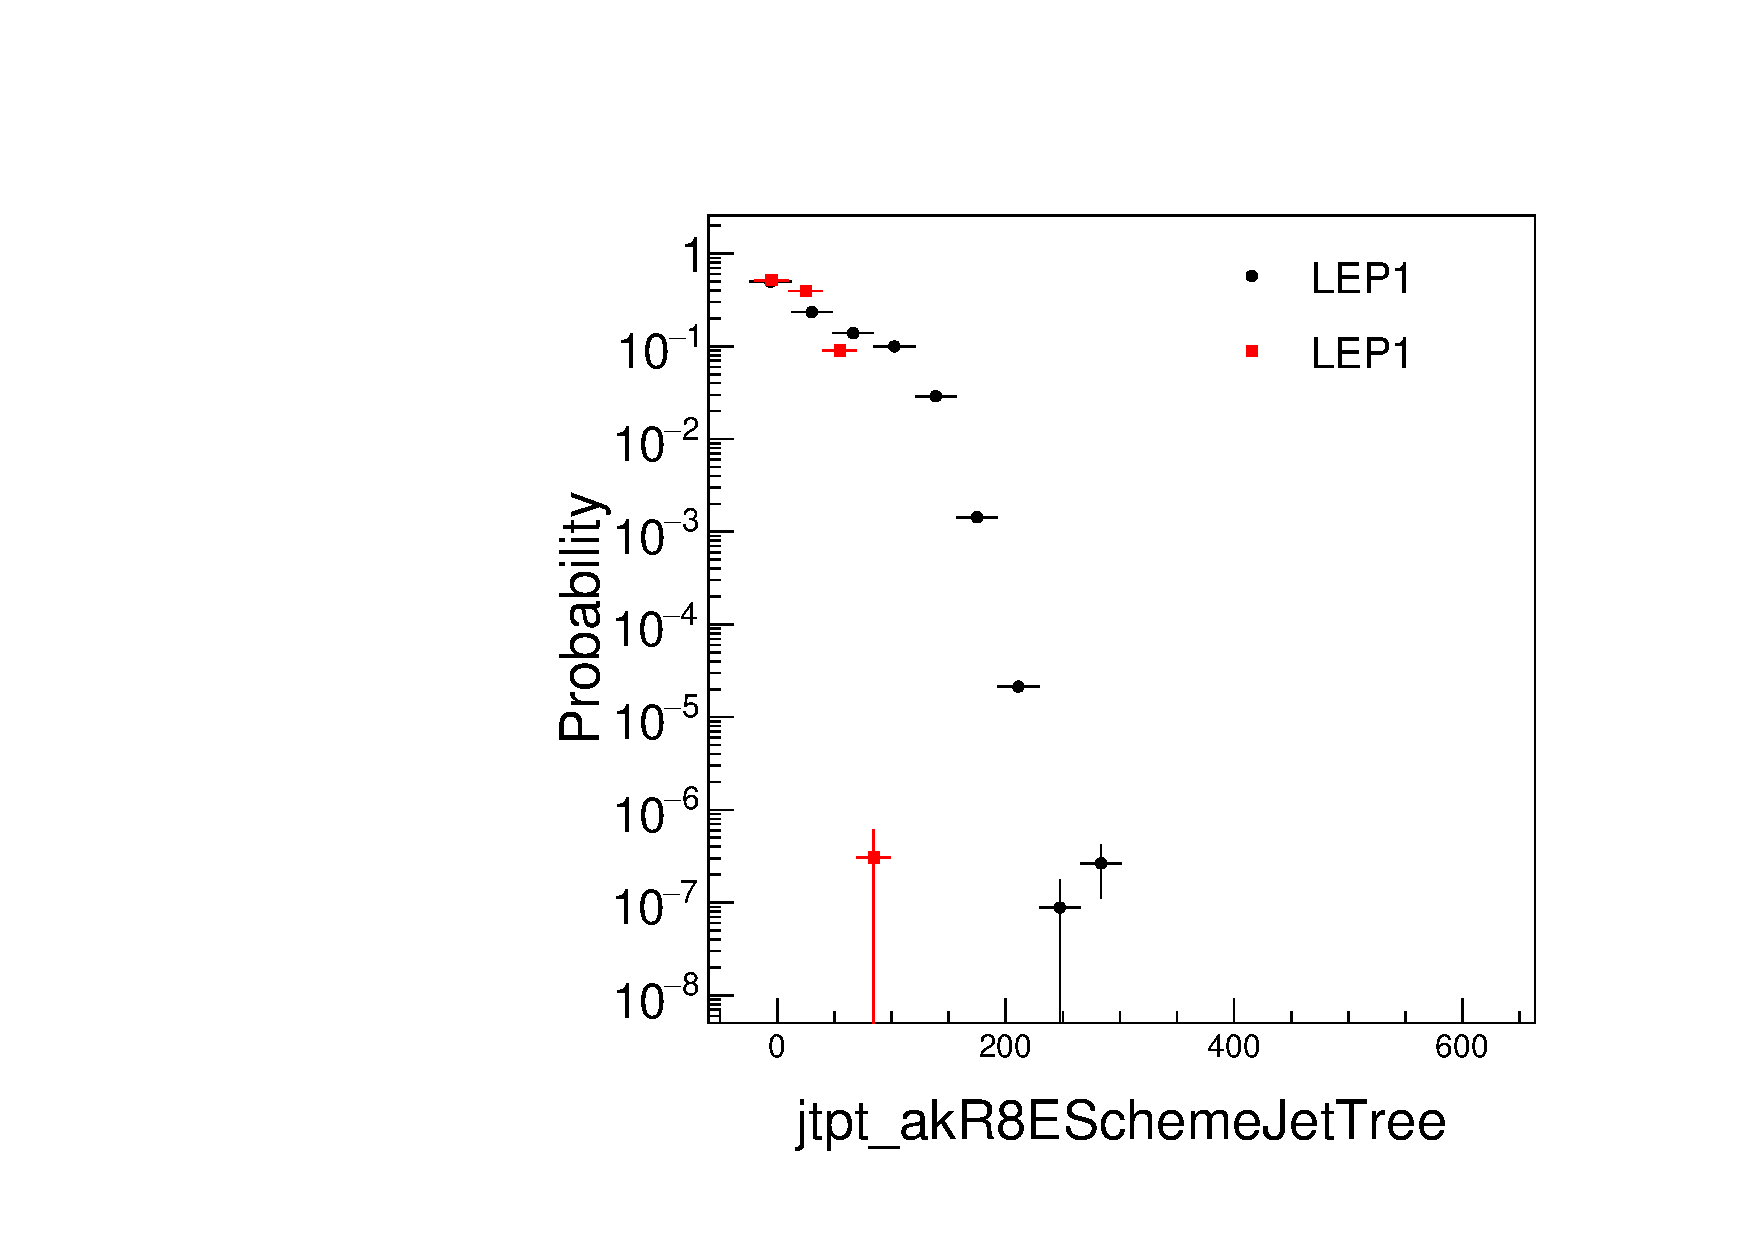
\includegraphics[width=.25\textwidth]{images/DQC/LEP1/jtpt_akR8ESchemeJetTree.pdf}}\hfill
\subfloat{\label{sfig:c}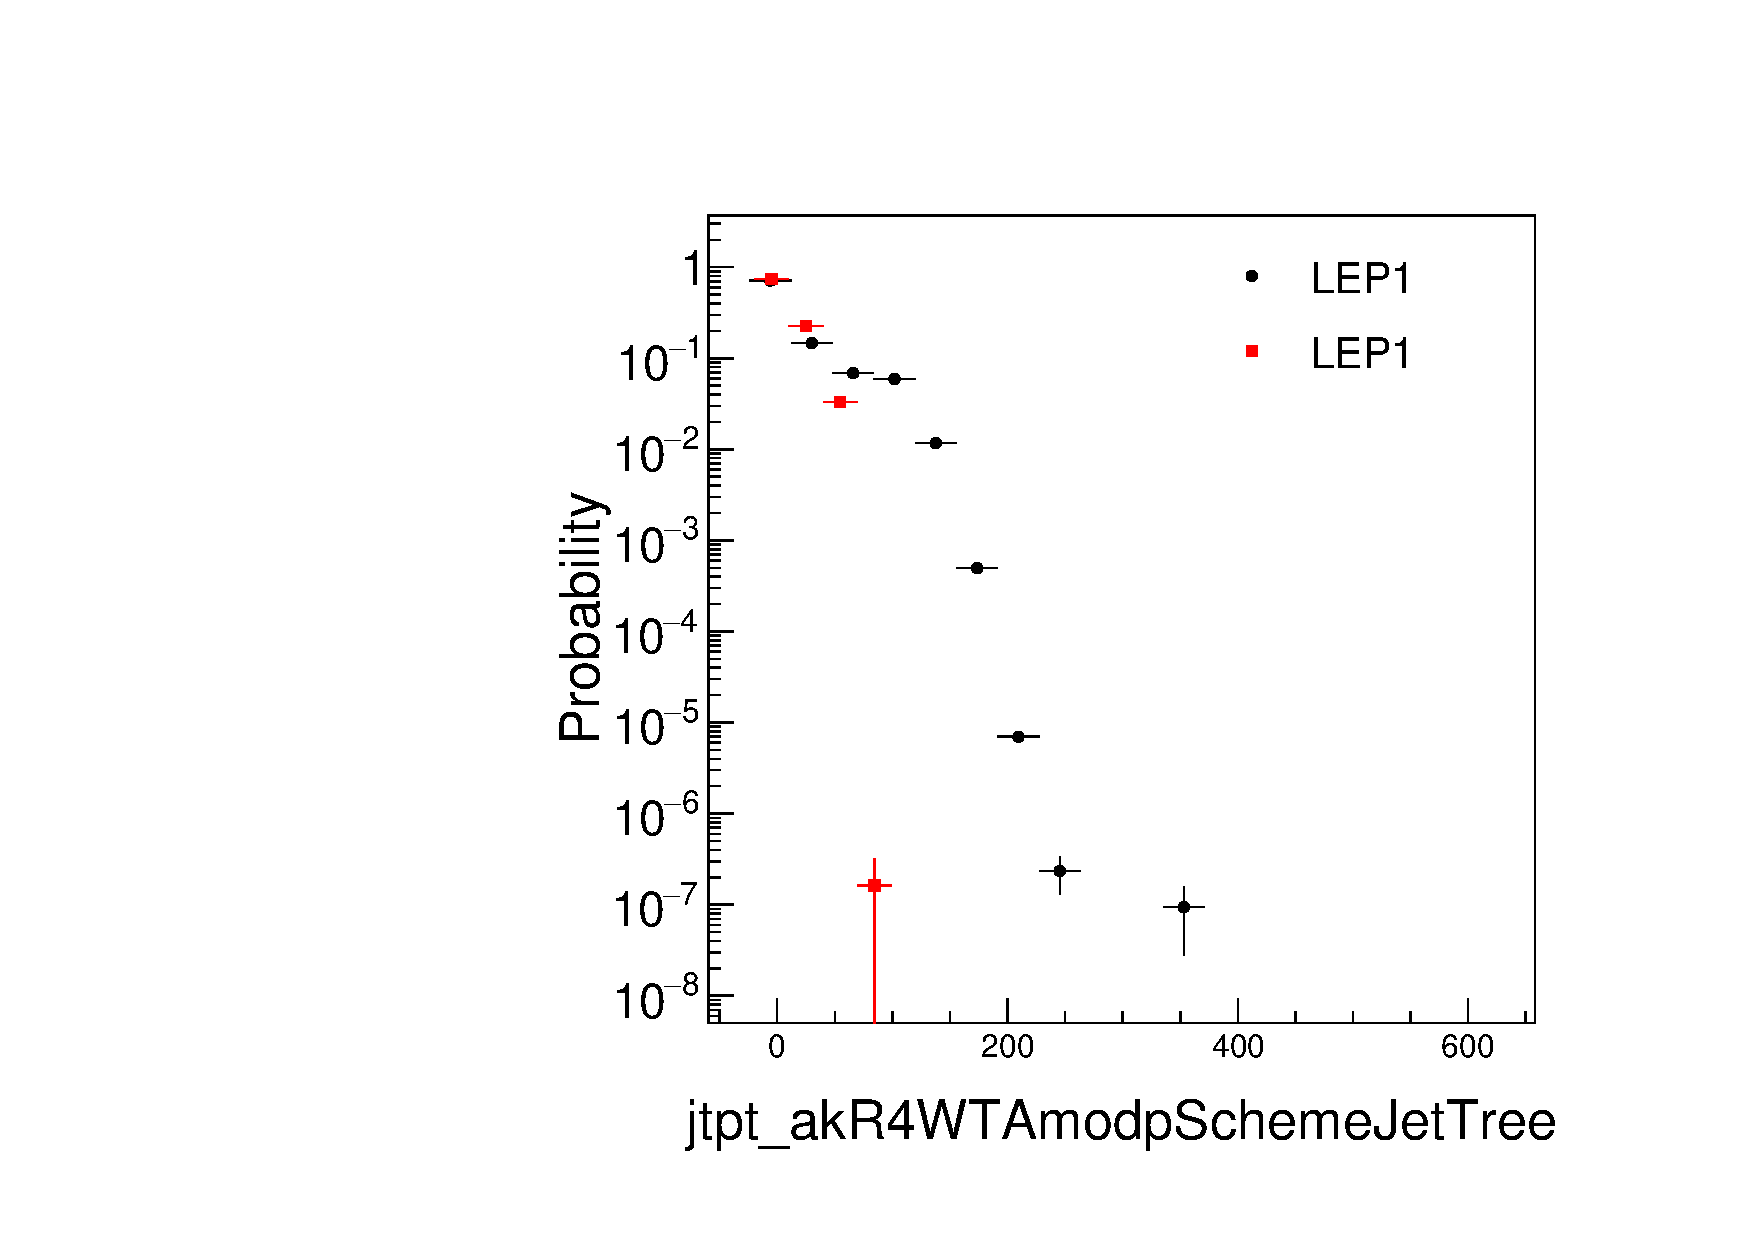
\includegraphics[width=.25\textwidth]{images/DQC/LEP1/jtpt_akR4WTAmodpSchemeJetTree.pdf}}\hfill
\subfloat{\label{sfig:d}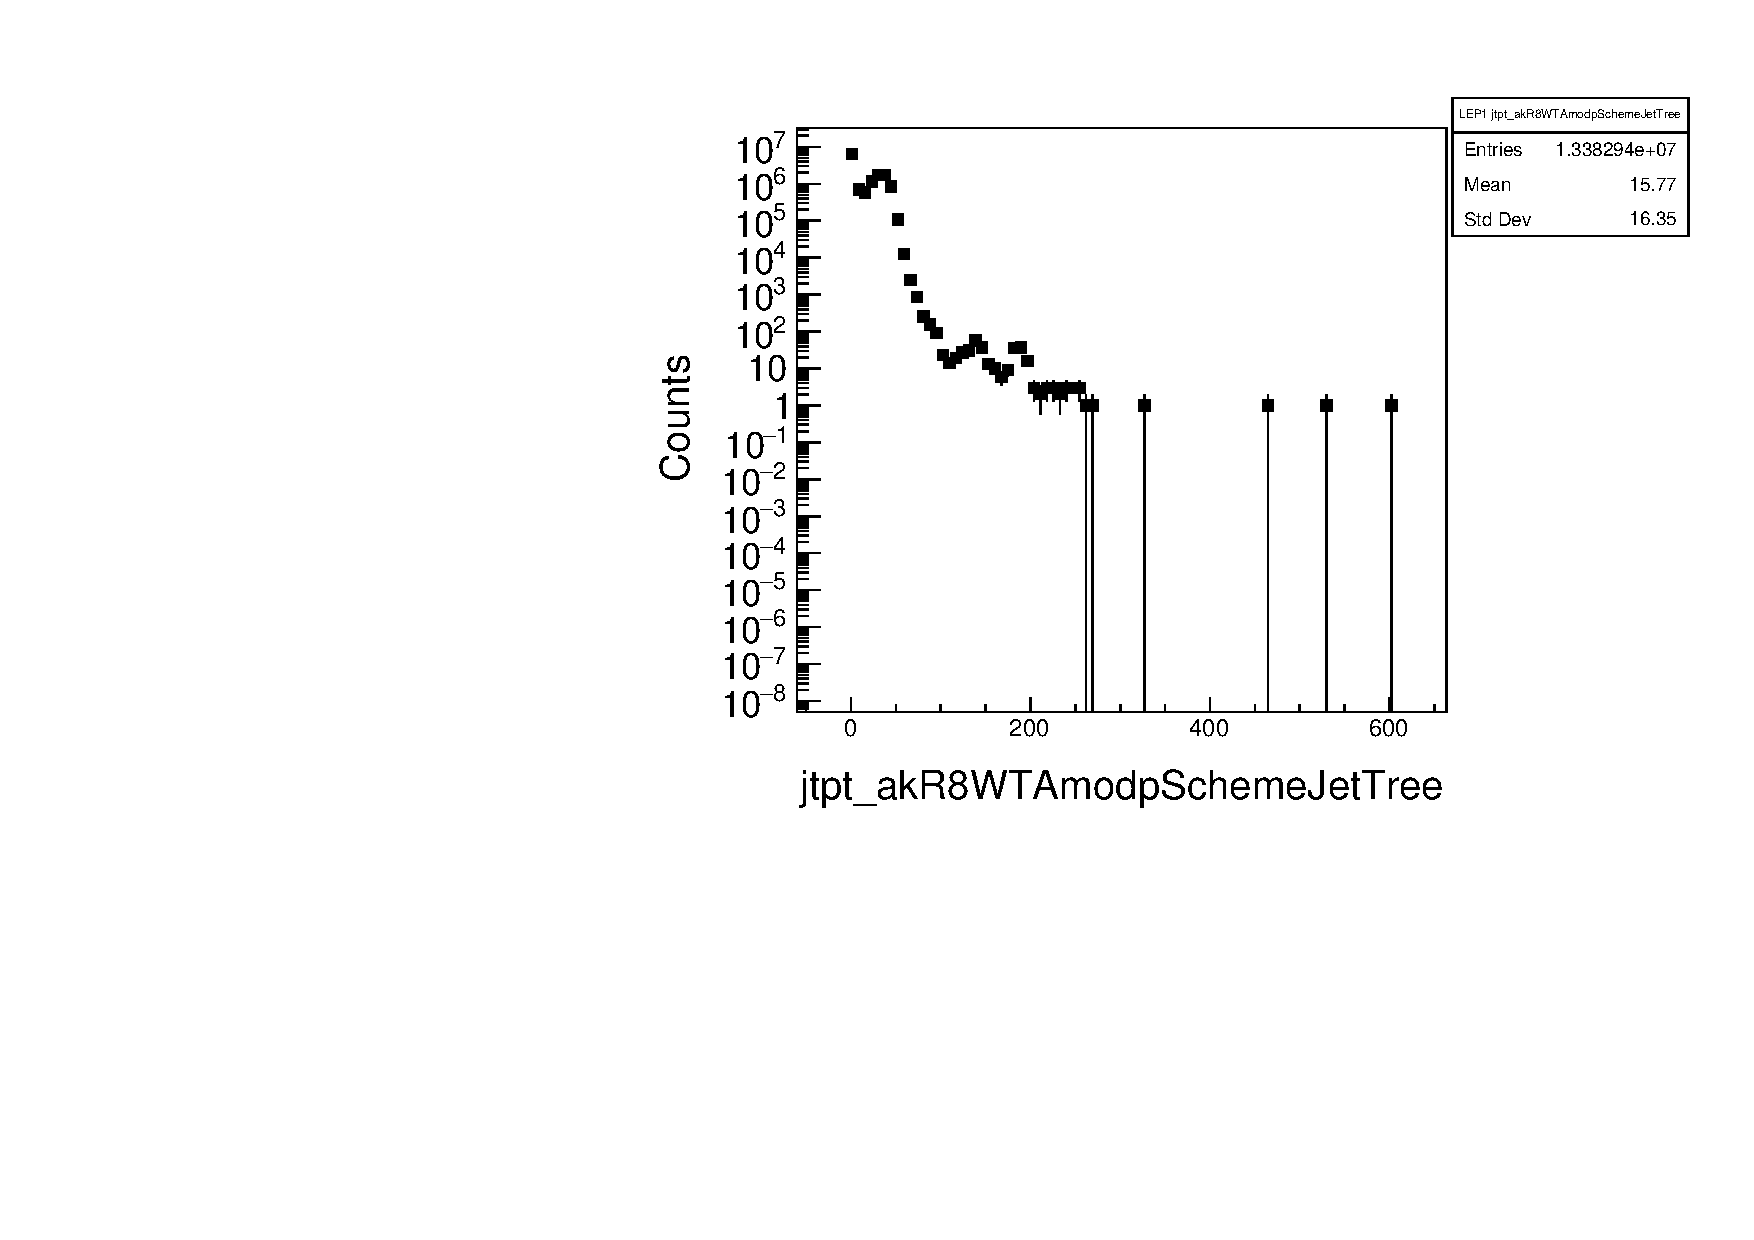
\includegraphics[width=.25\textwidth]{images/DQC/LEP1/jtpt_akR8WTAmodpSchemeJetTree.pdf}}\hfill %row end
\subfloat{\label{sfig:e}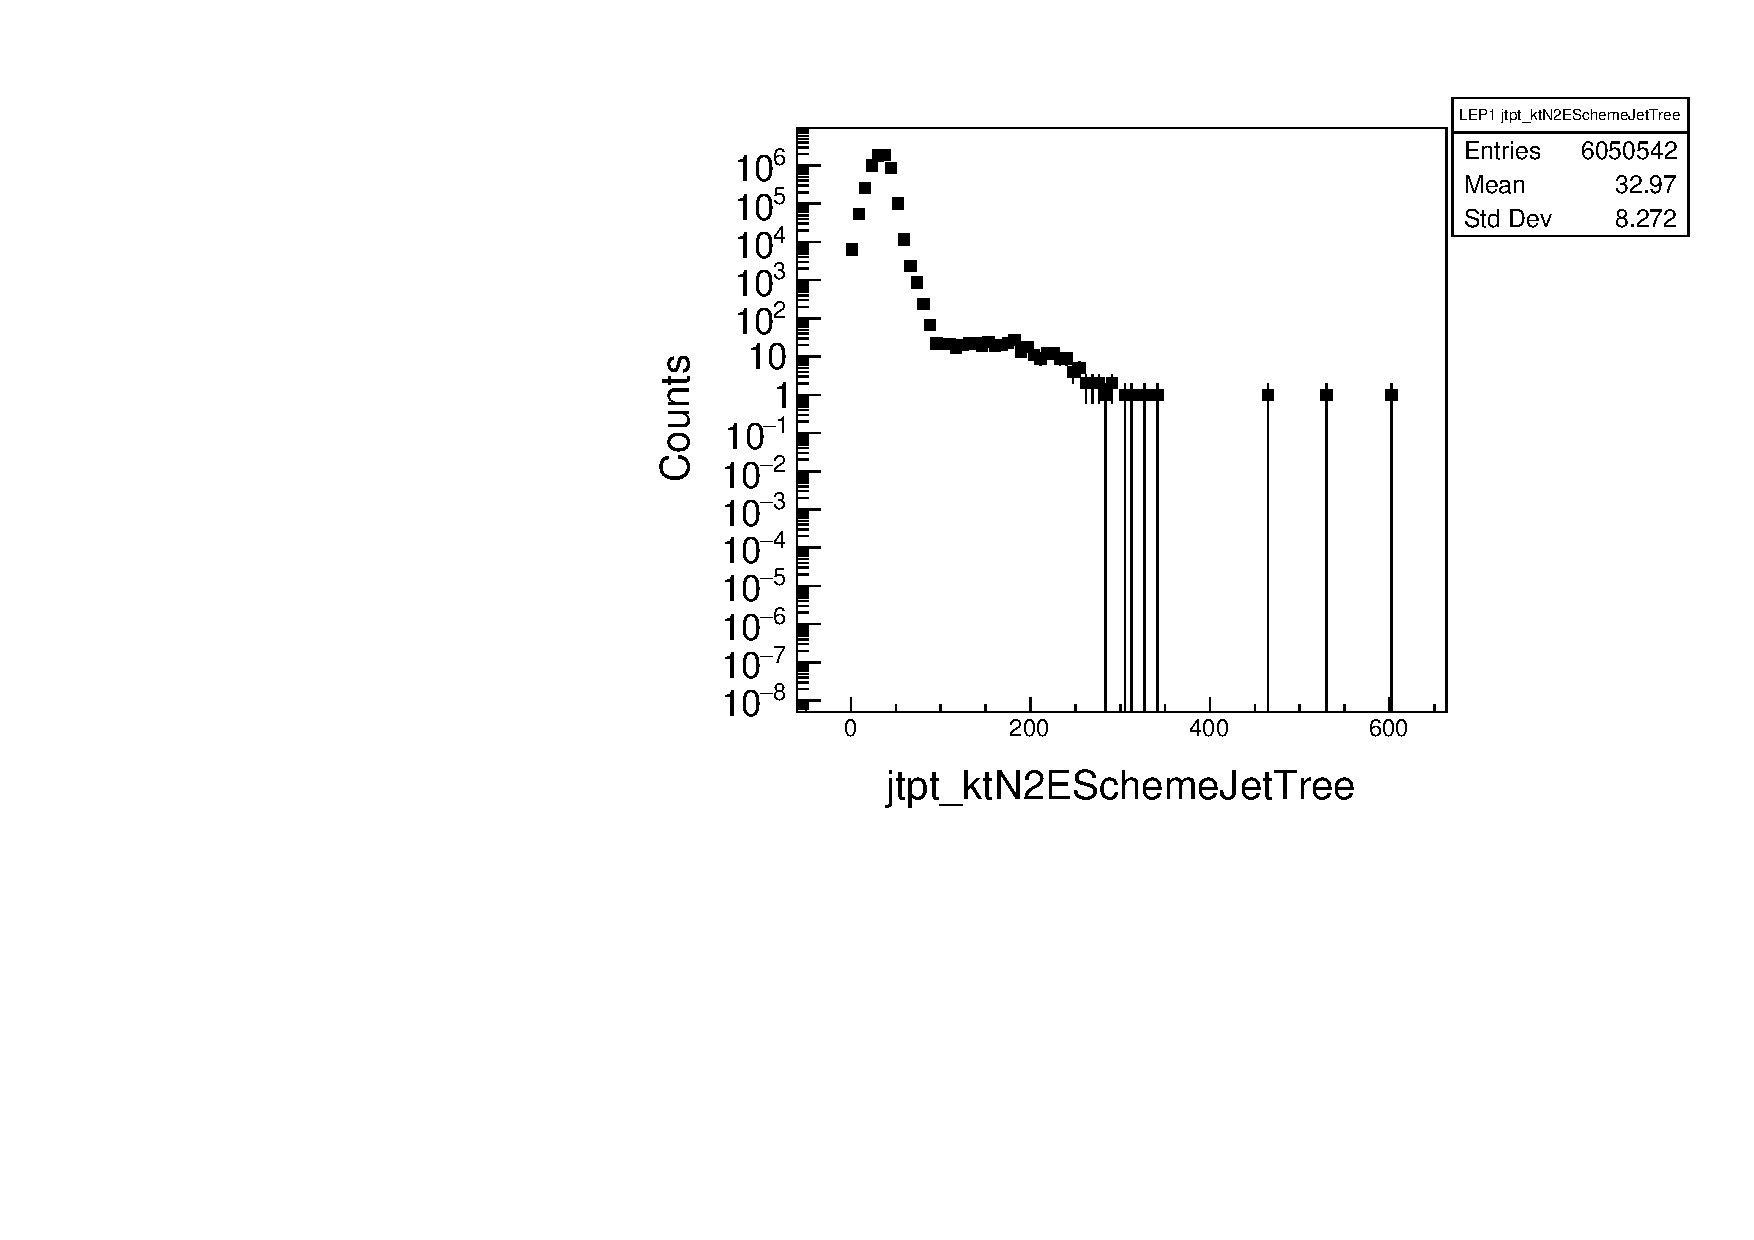
\includegraphics[width=.25\textwidth]{images/DQC/LEP1/jtpt_ktN2ESchemeJetTree.pdf}}\hfill
\subfloat{\label{sfig:f}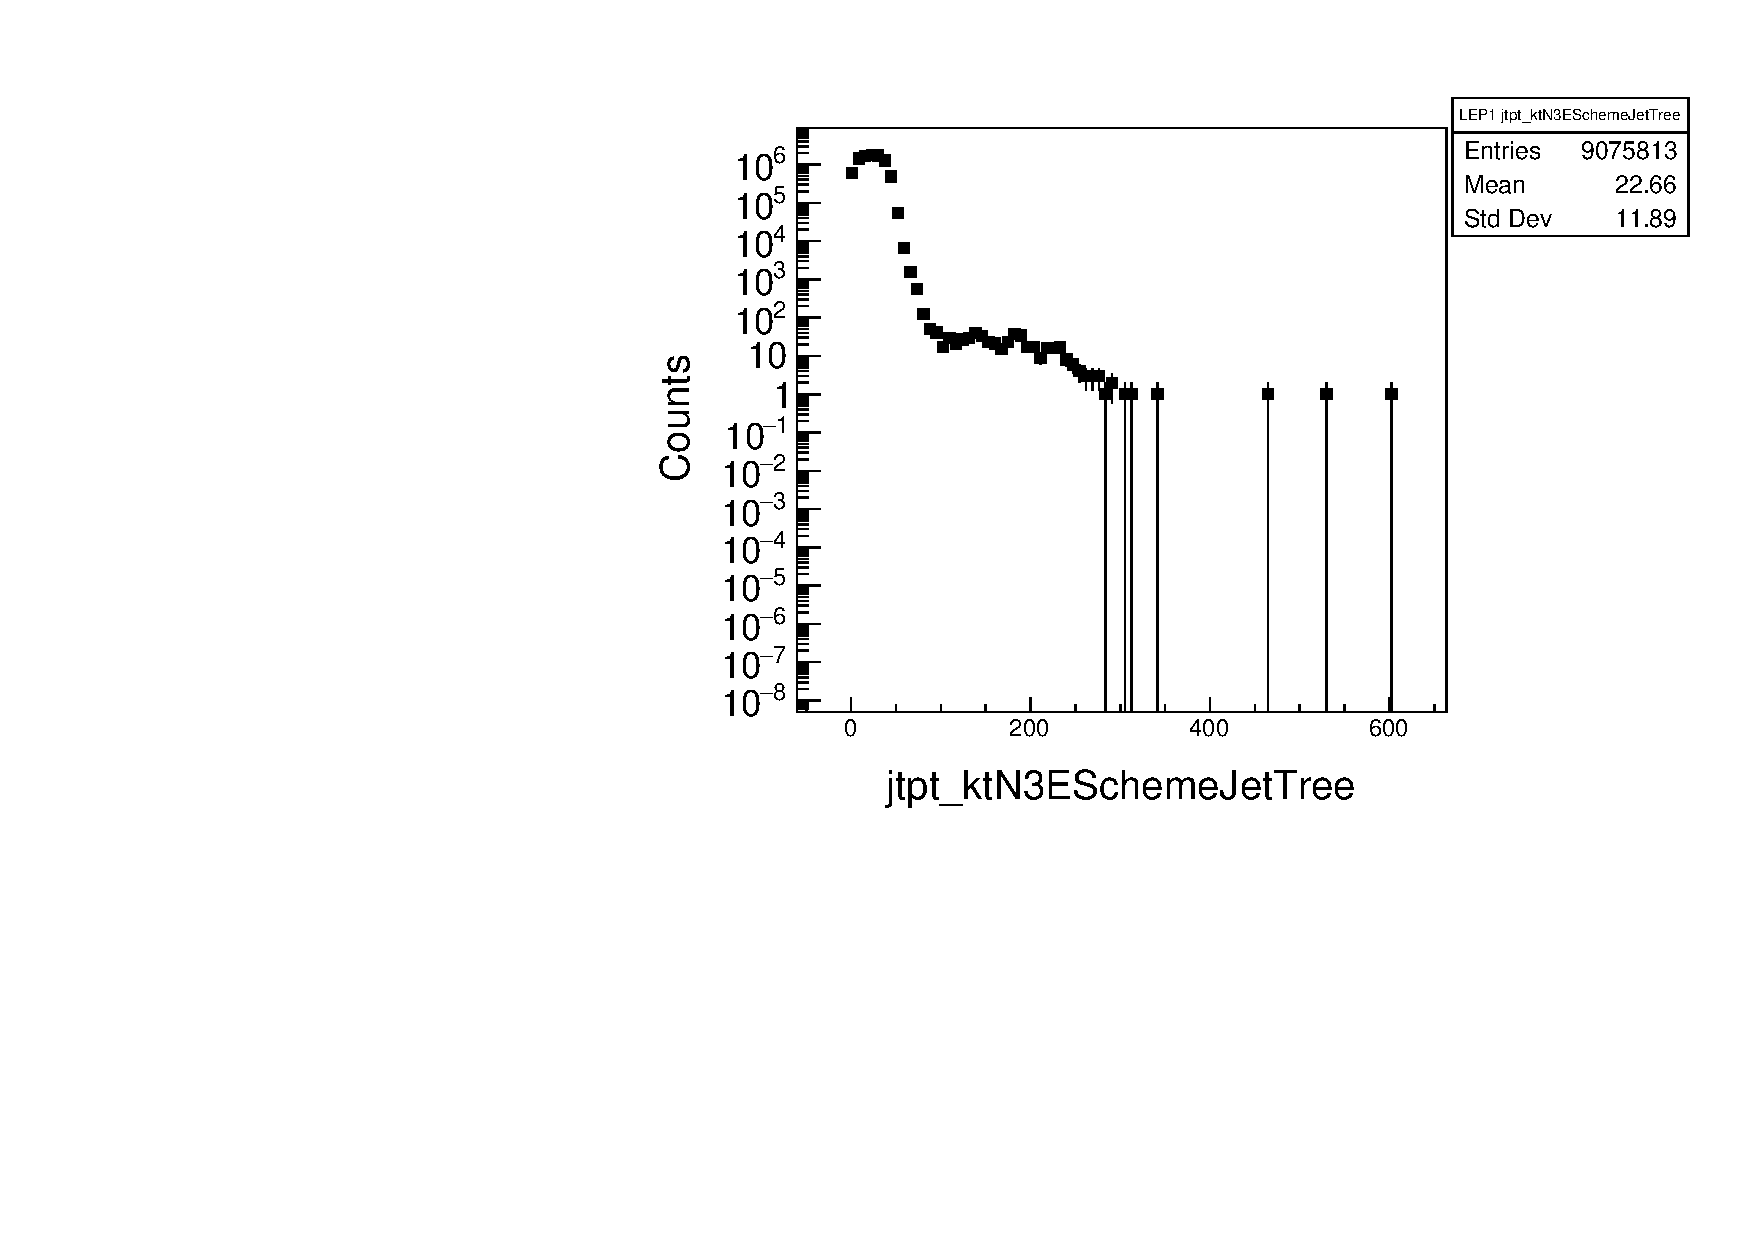
\includegraphics[width=.25\textwidth]{images/DQC/LEP1/jtpt_ktN3ESchemeJetTree.pdf}}\hfill
\subfloat{\label{sfig:g}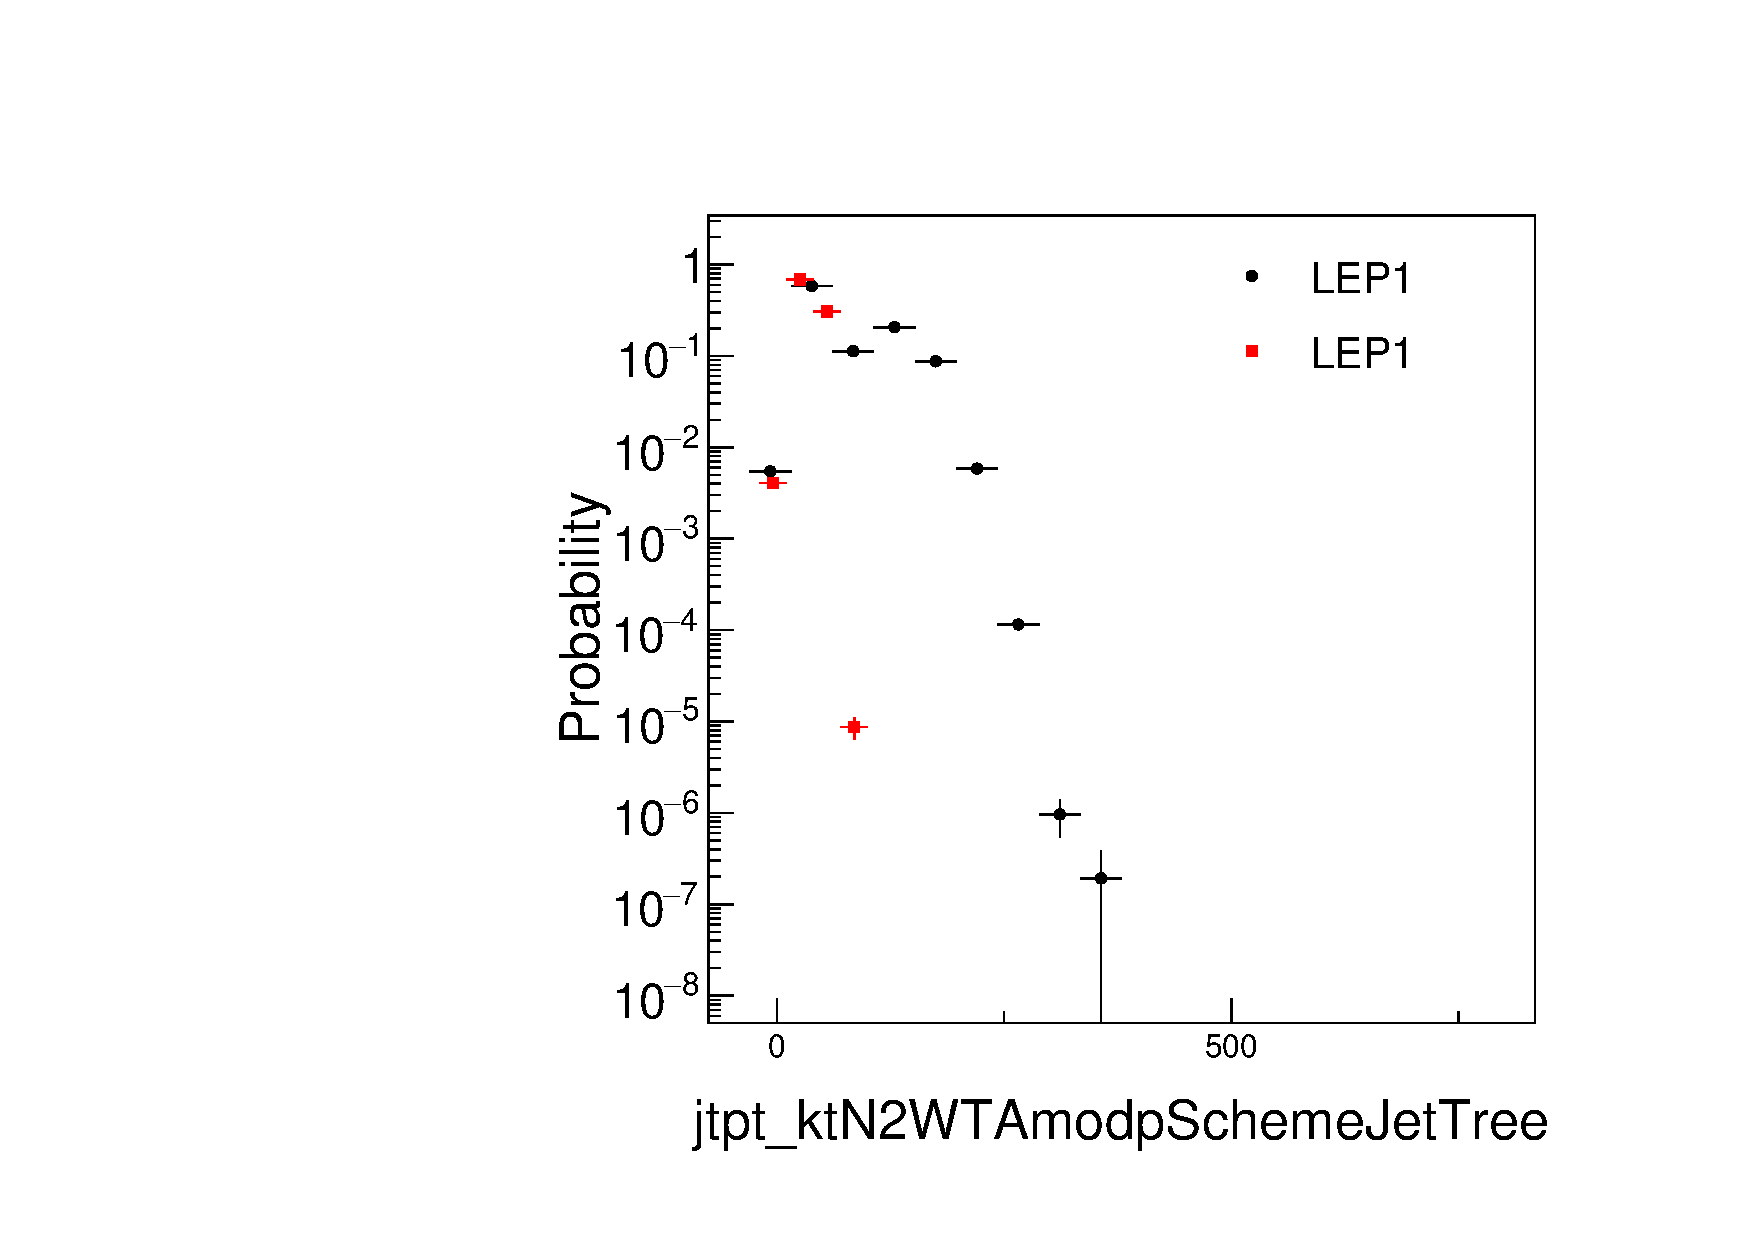
\includegraphics[width=.25\textwidth]{images/DQC/LEP1/jtpt_ktN2WTAmodpSchemeJetTree.pdf}}\hfill
\subfloat{\label{sfig:h}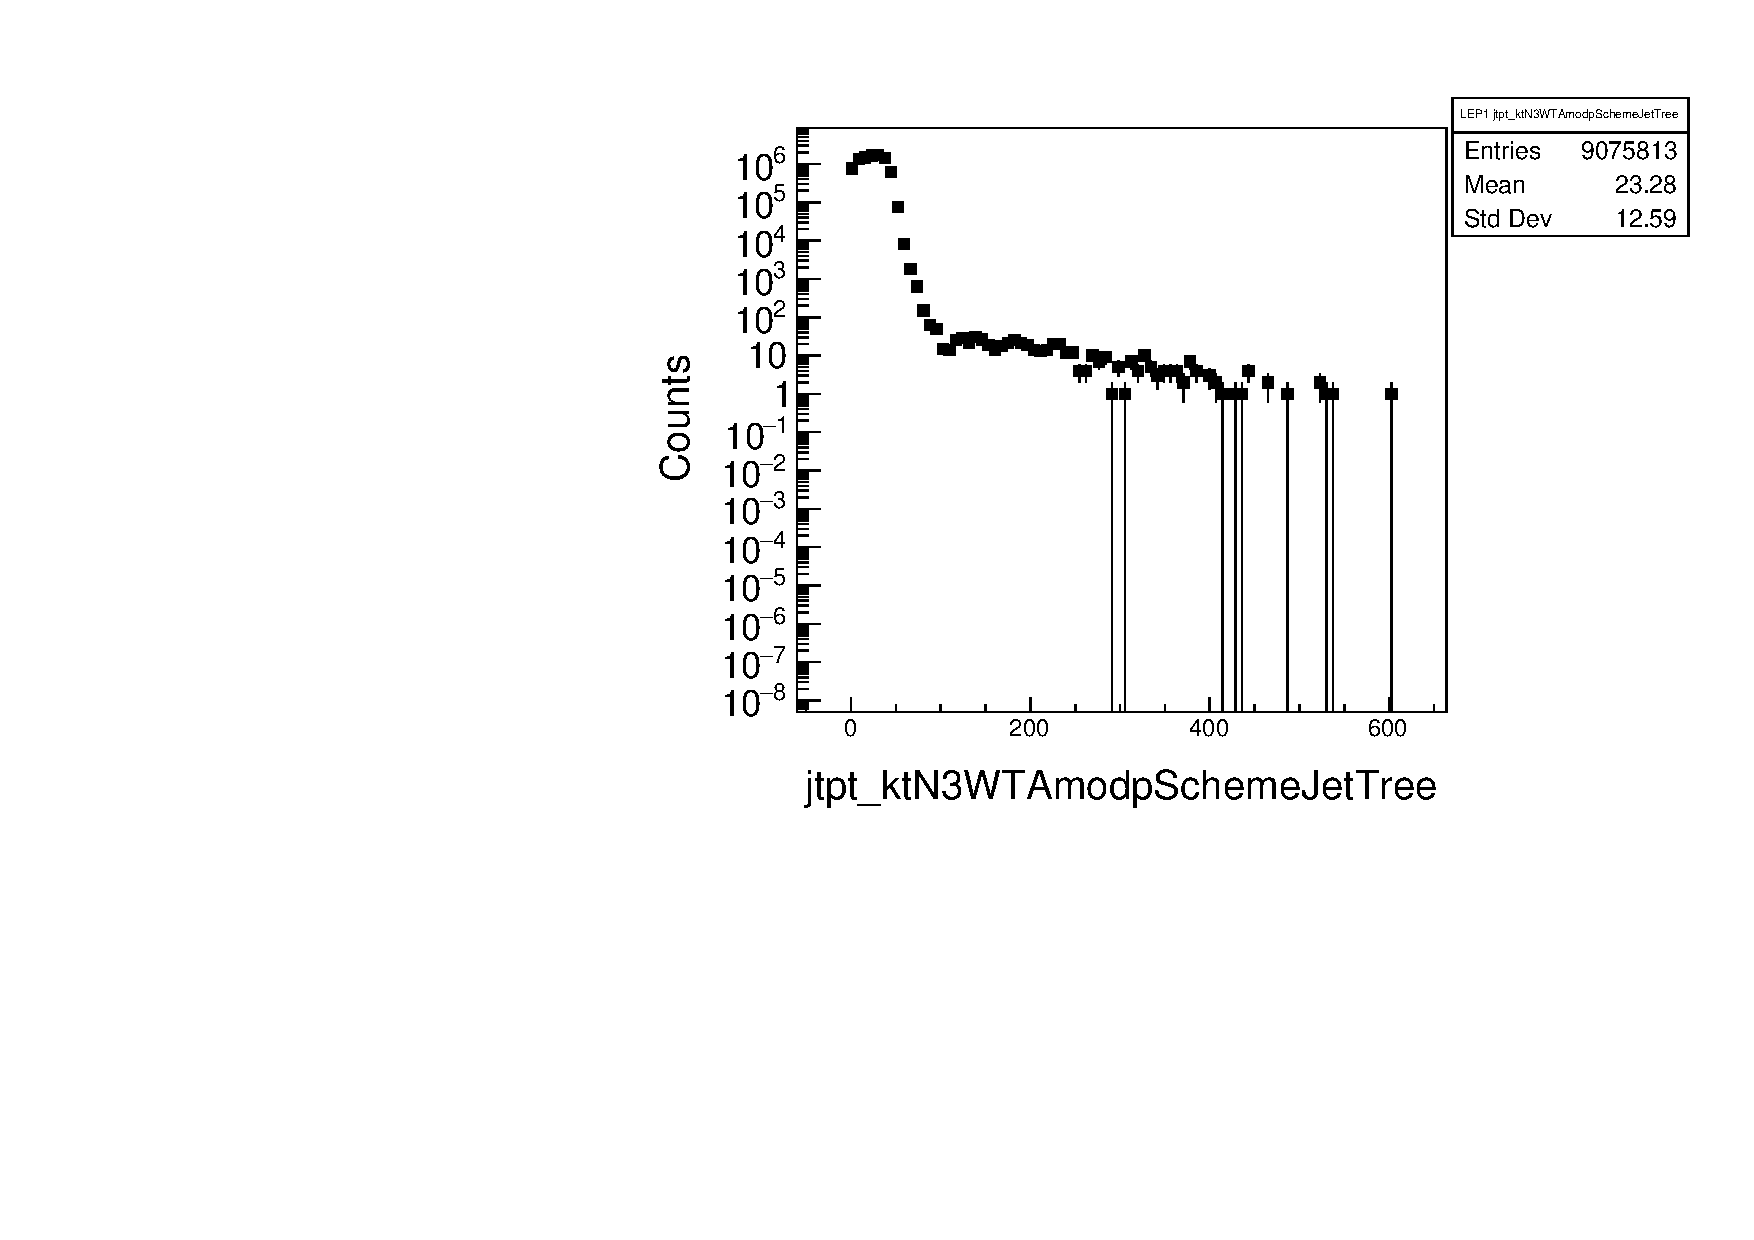
\includegraphics[width=.25\textwidth]{images/DQC/LEP1/jtpt_ktN3WTAmodpSchemeJetTree.pdf}}\hfill
\caption{LEP1 Jet $p_t$ distributions. Top row: anti-$k_t$, left to right: $R=0.4$, $E$ scheme; $R=0.8$, $E$ scheme; $R=0.4$, WTA mod p scheme; $R=0.8$, WTA mod p scheme. Bottom row: $k_t$, left to right: $N=2$, $E$ scheme; $N=3$, $E$ scheme; $N=2$, WTA mod p scheme; $N=3$; WTA mod p scheme.}  
\end{figure}

\begin{figure}[H]
\centering
\subfloat{\label{sfig:a}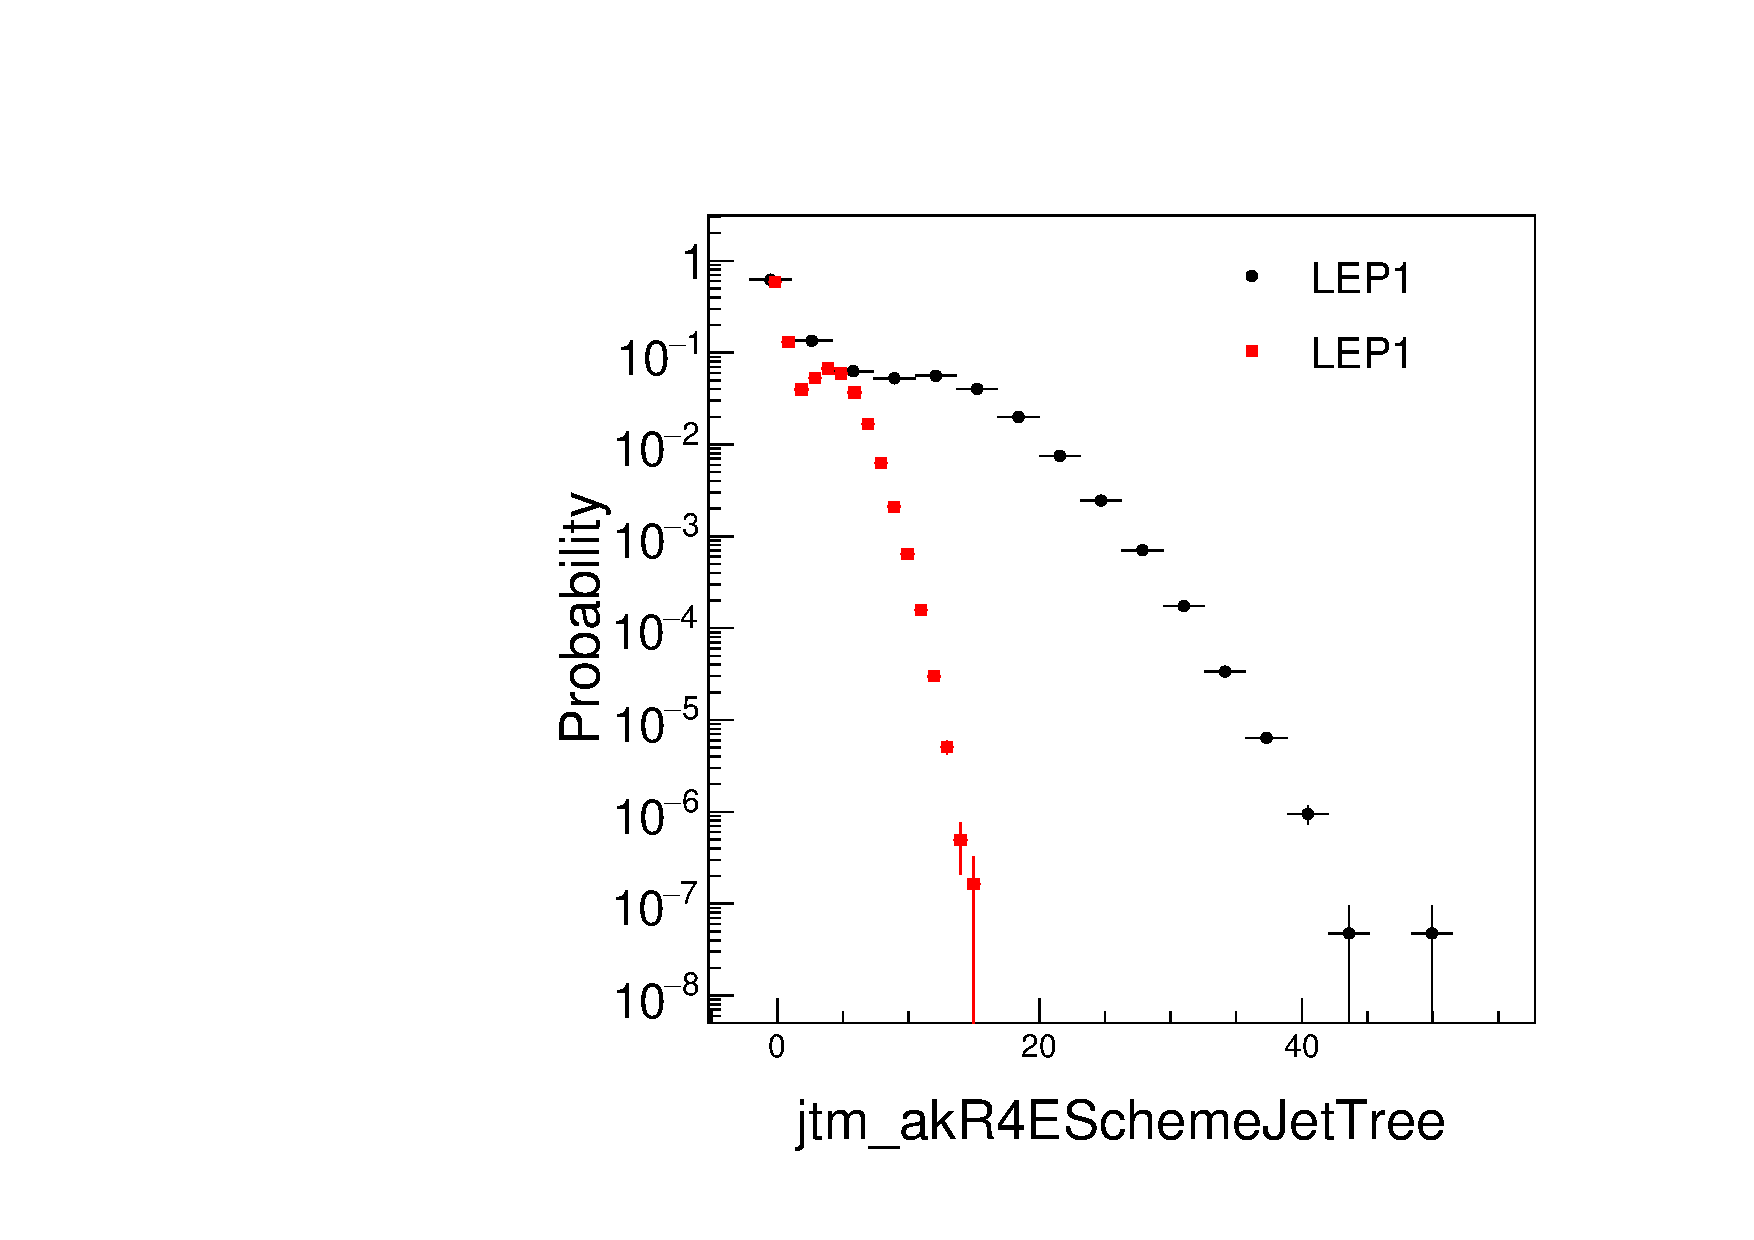
\includegraphics[width=.25\textwidth]{images/DQC/LEP1/jtm_akR4ESchemeJetTree.pdf}}\hfill
\subfloat{\label{sfig:b}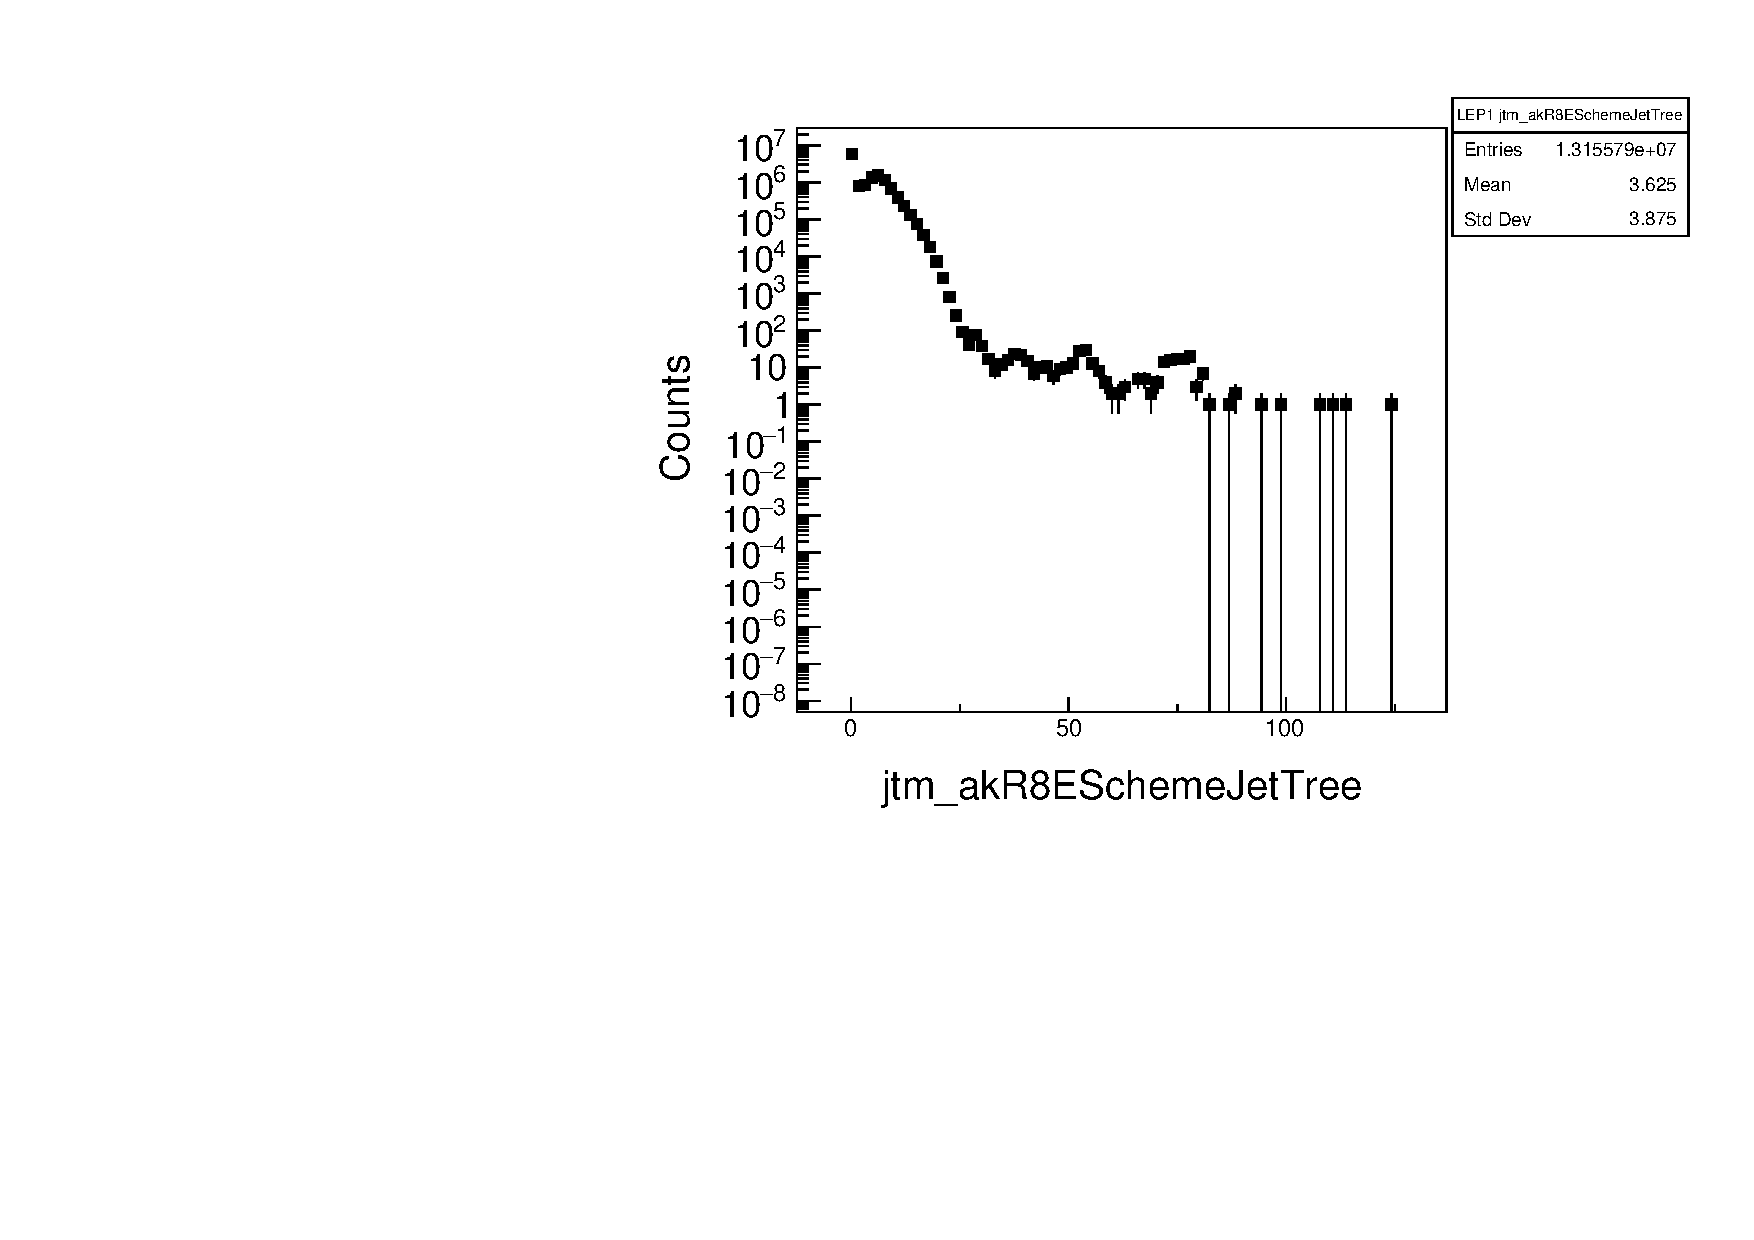
\includegraphics[width=.25\textwidth]{images/DQC/LEP1/jtm_akR8ESchemeJetTree.pdf}}\hfill
\subfloat{\label{sfig:c}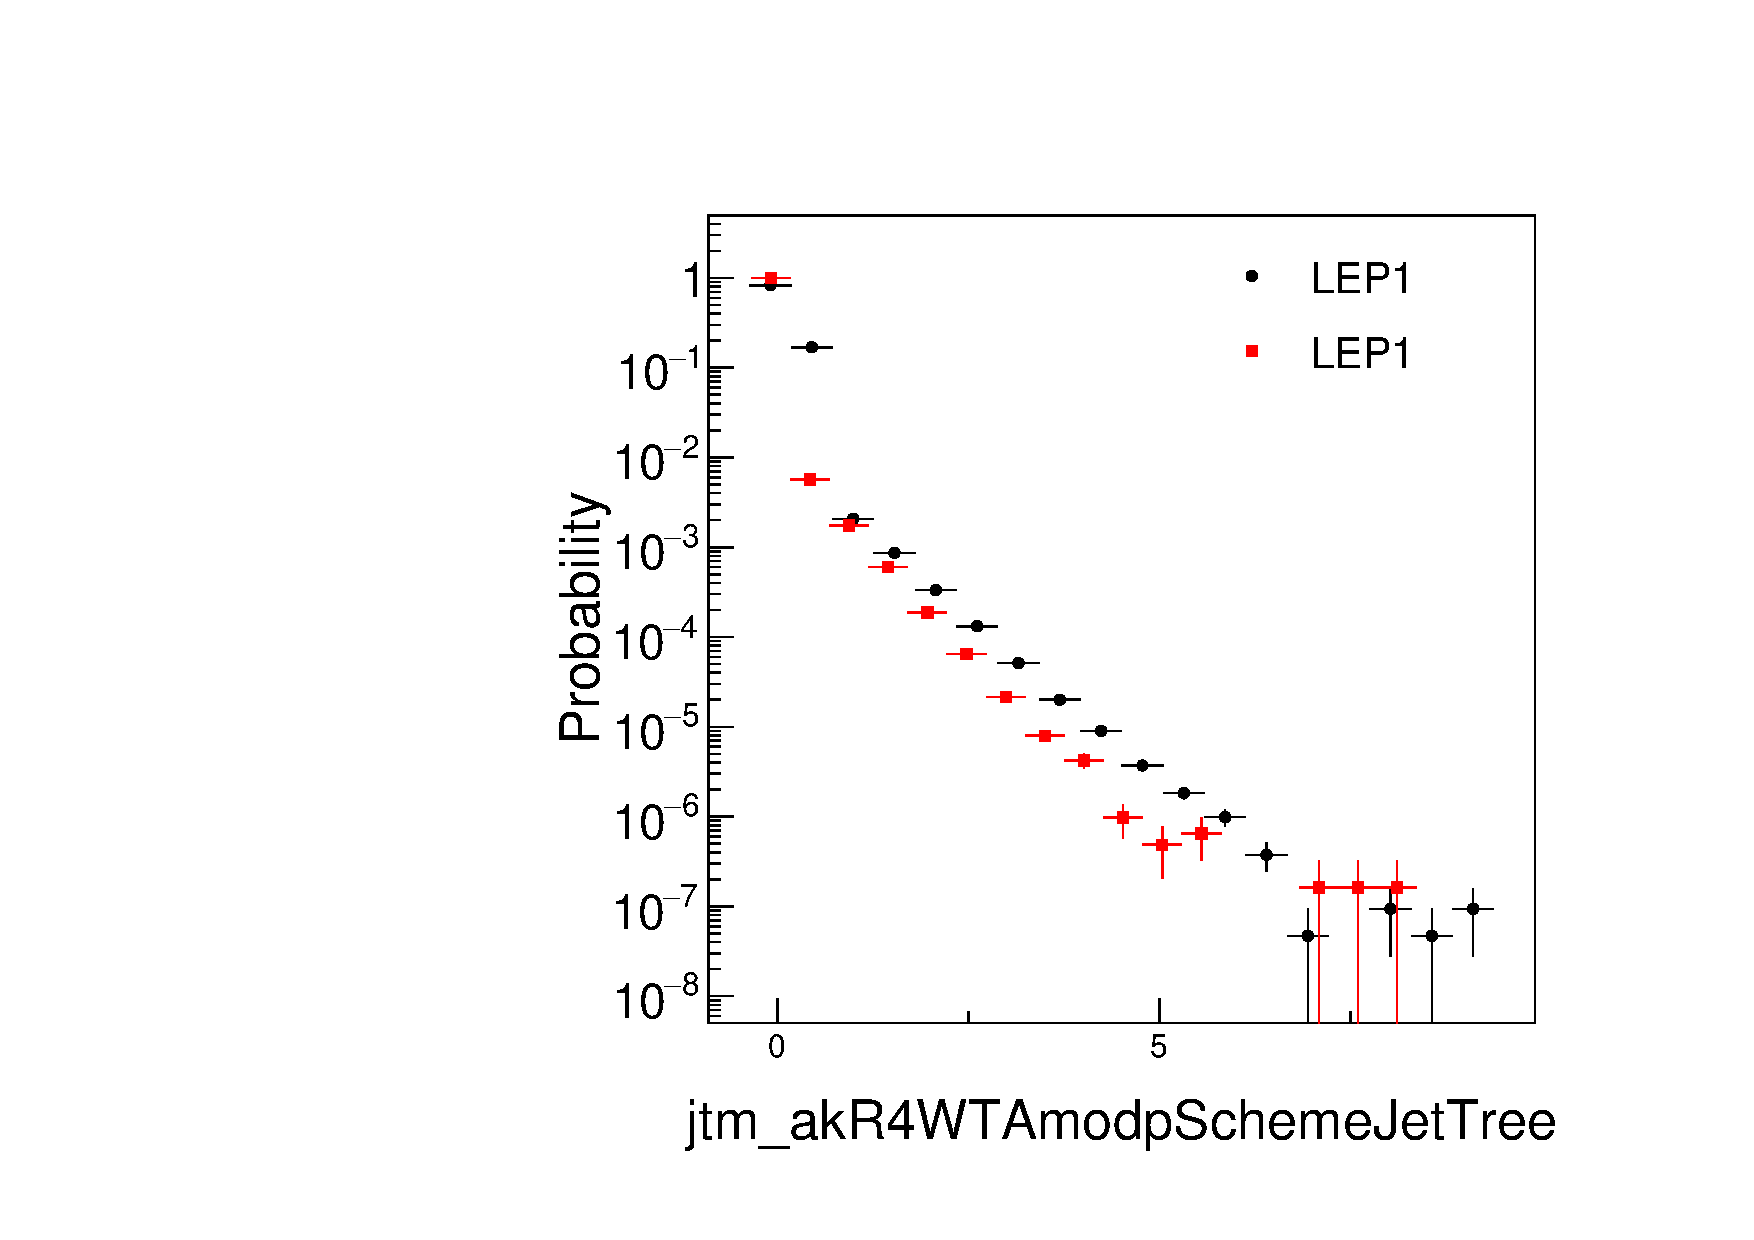
\includegraphics[width=.25\textwidth]{images/DQC/LEP1/jtm_akR4WTAmodpSchemeJetTree.pdf}}\hfill
\subfloat{\label{sfig:d}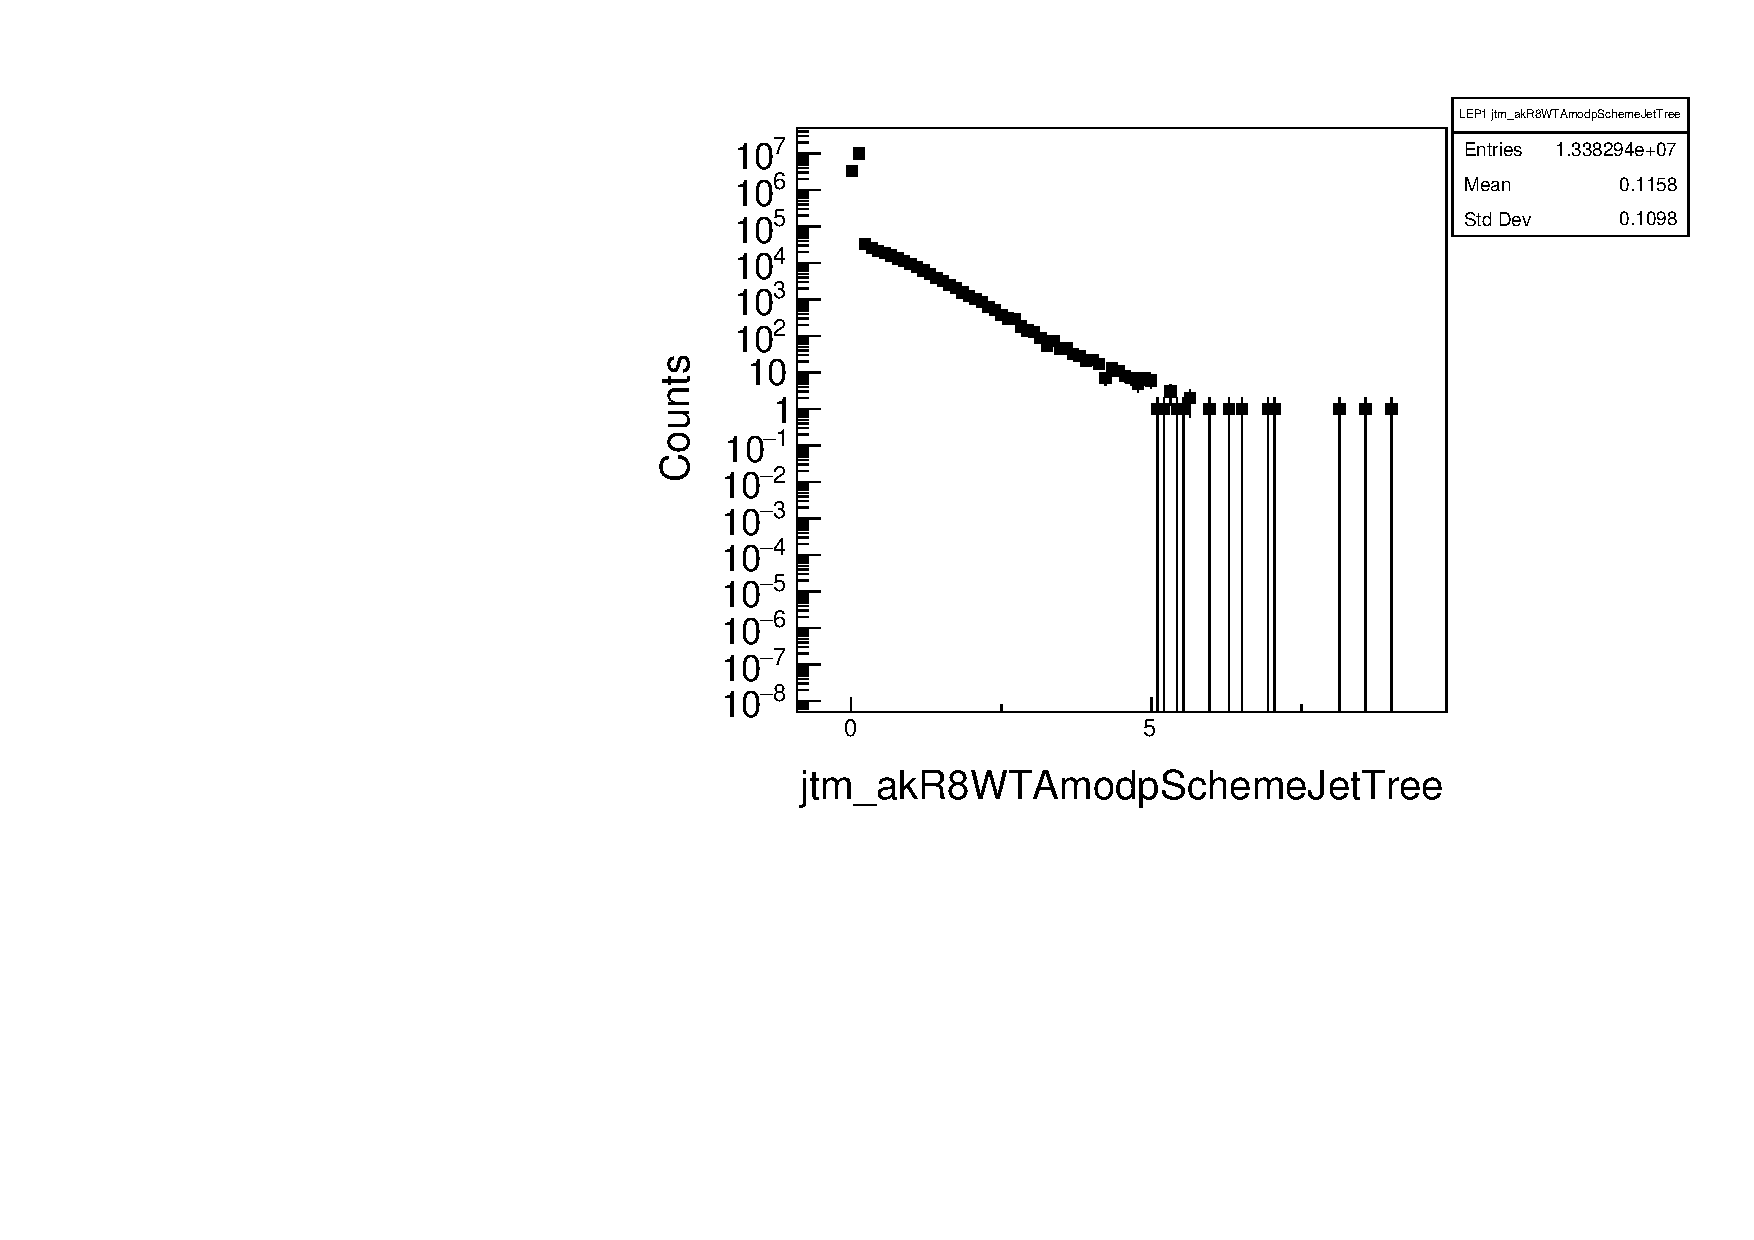
\includegraphics[width=.25\textwidth]{images/DQC/LEP1/jtm_akR8WTAmodpSchemeJetTree.pdf}}\hfill %row end
\subfloat{\label{sfig:e}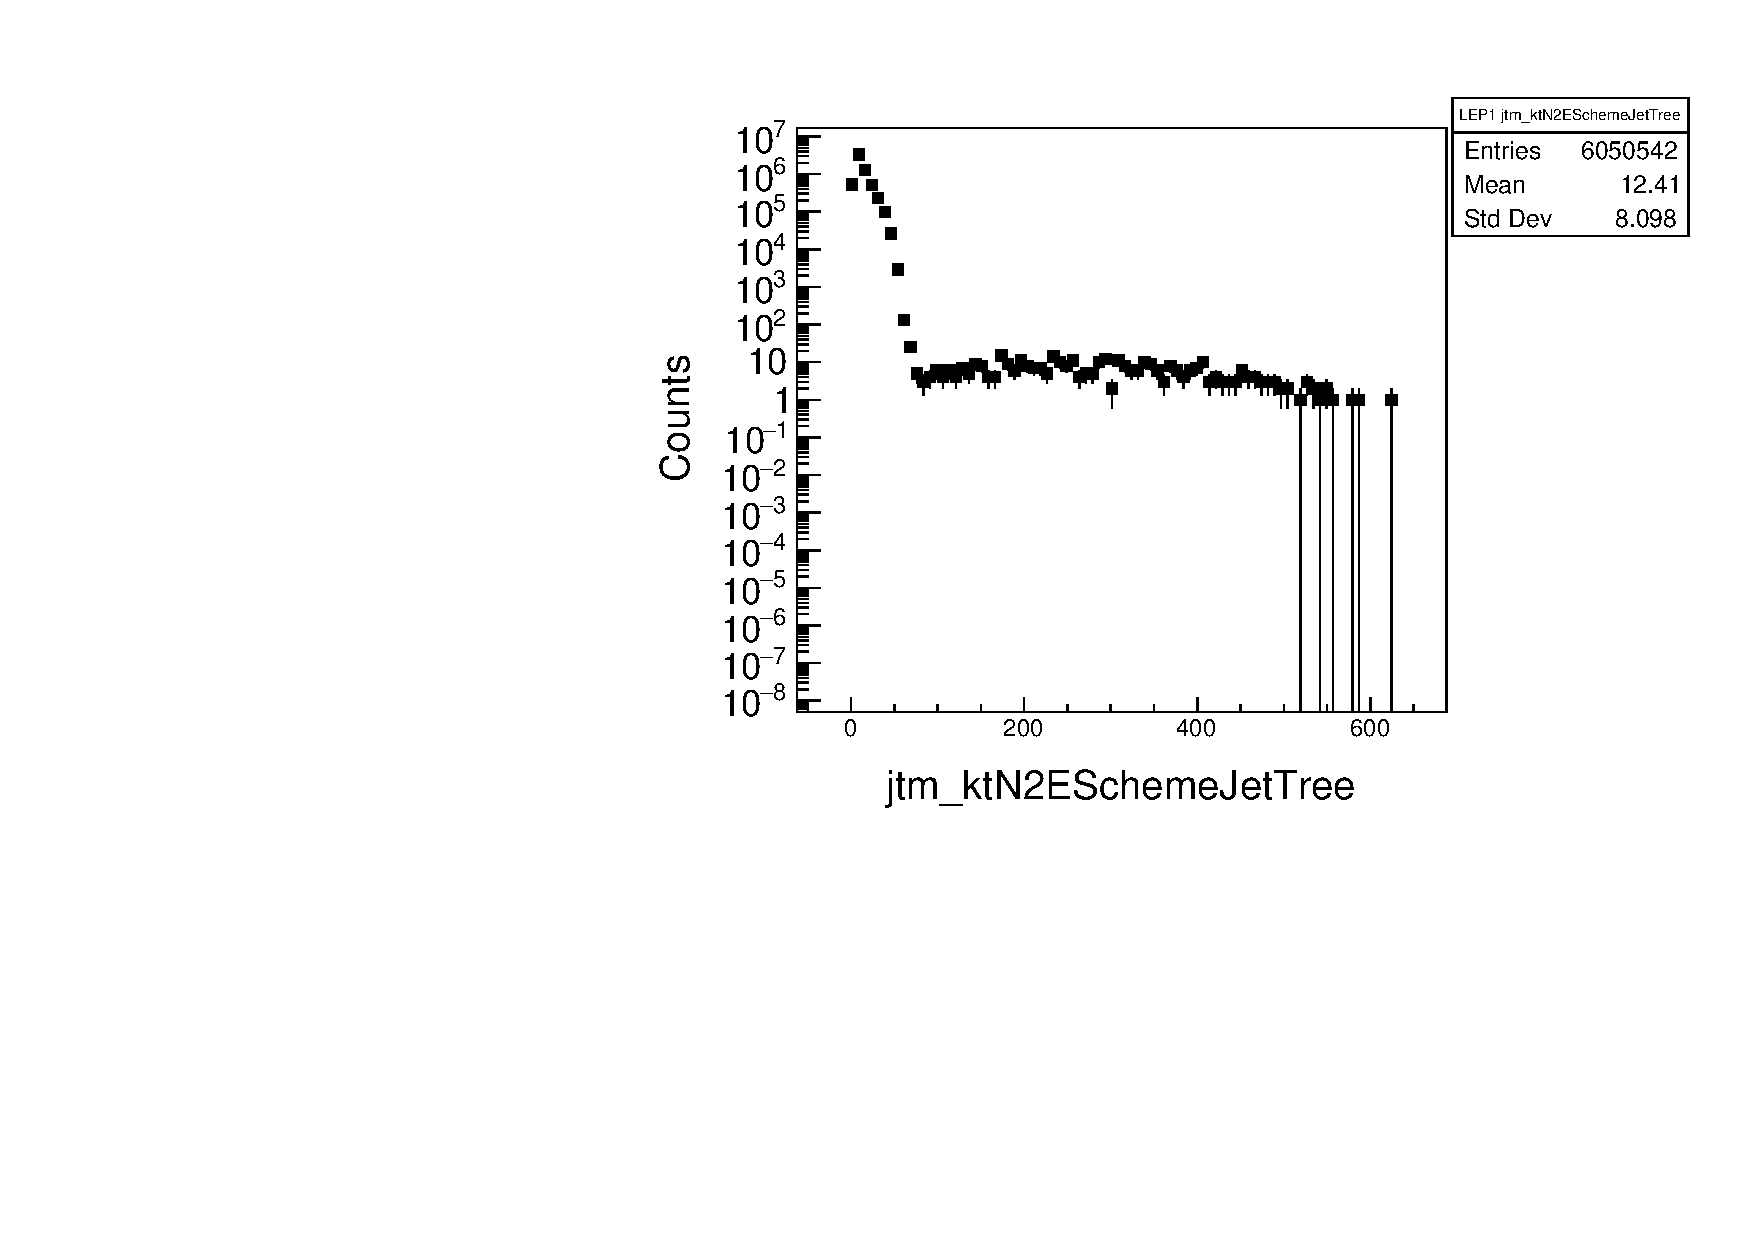
\includegraphics[width=.25\textwidth]{images/DQC/LEP1/jtm_ktN2ESchemeJetTree.pdf}}\hfill
\subfloat{\label{sfig:f}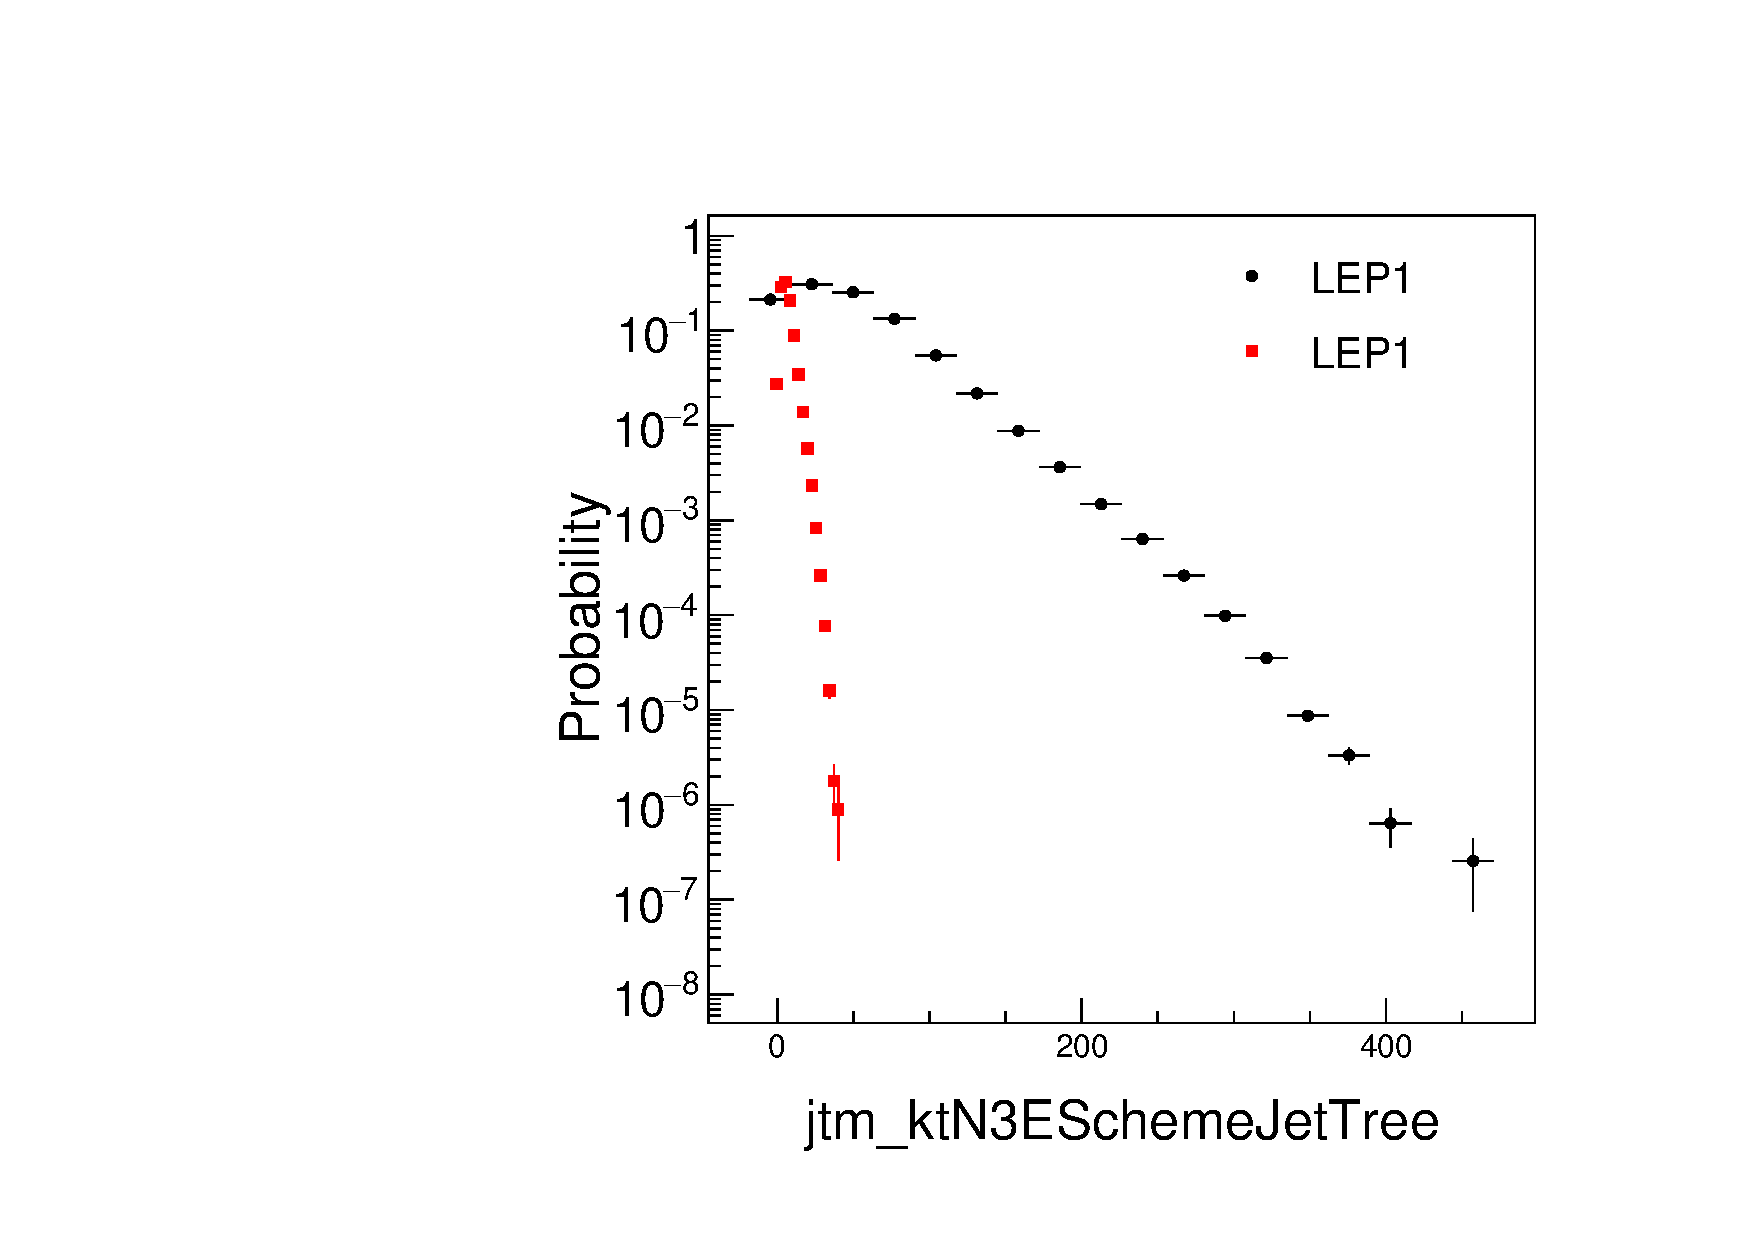
\includegraphics[width=.25\textwidth]{images/DQC/LEP1/jtm_ktN3ESchemeJetTree.pdf}}\hfill
\subfloat{\label{sfig:g}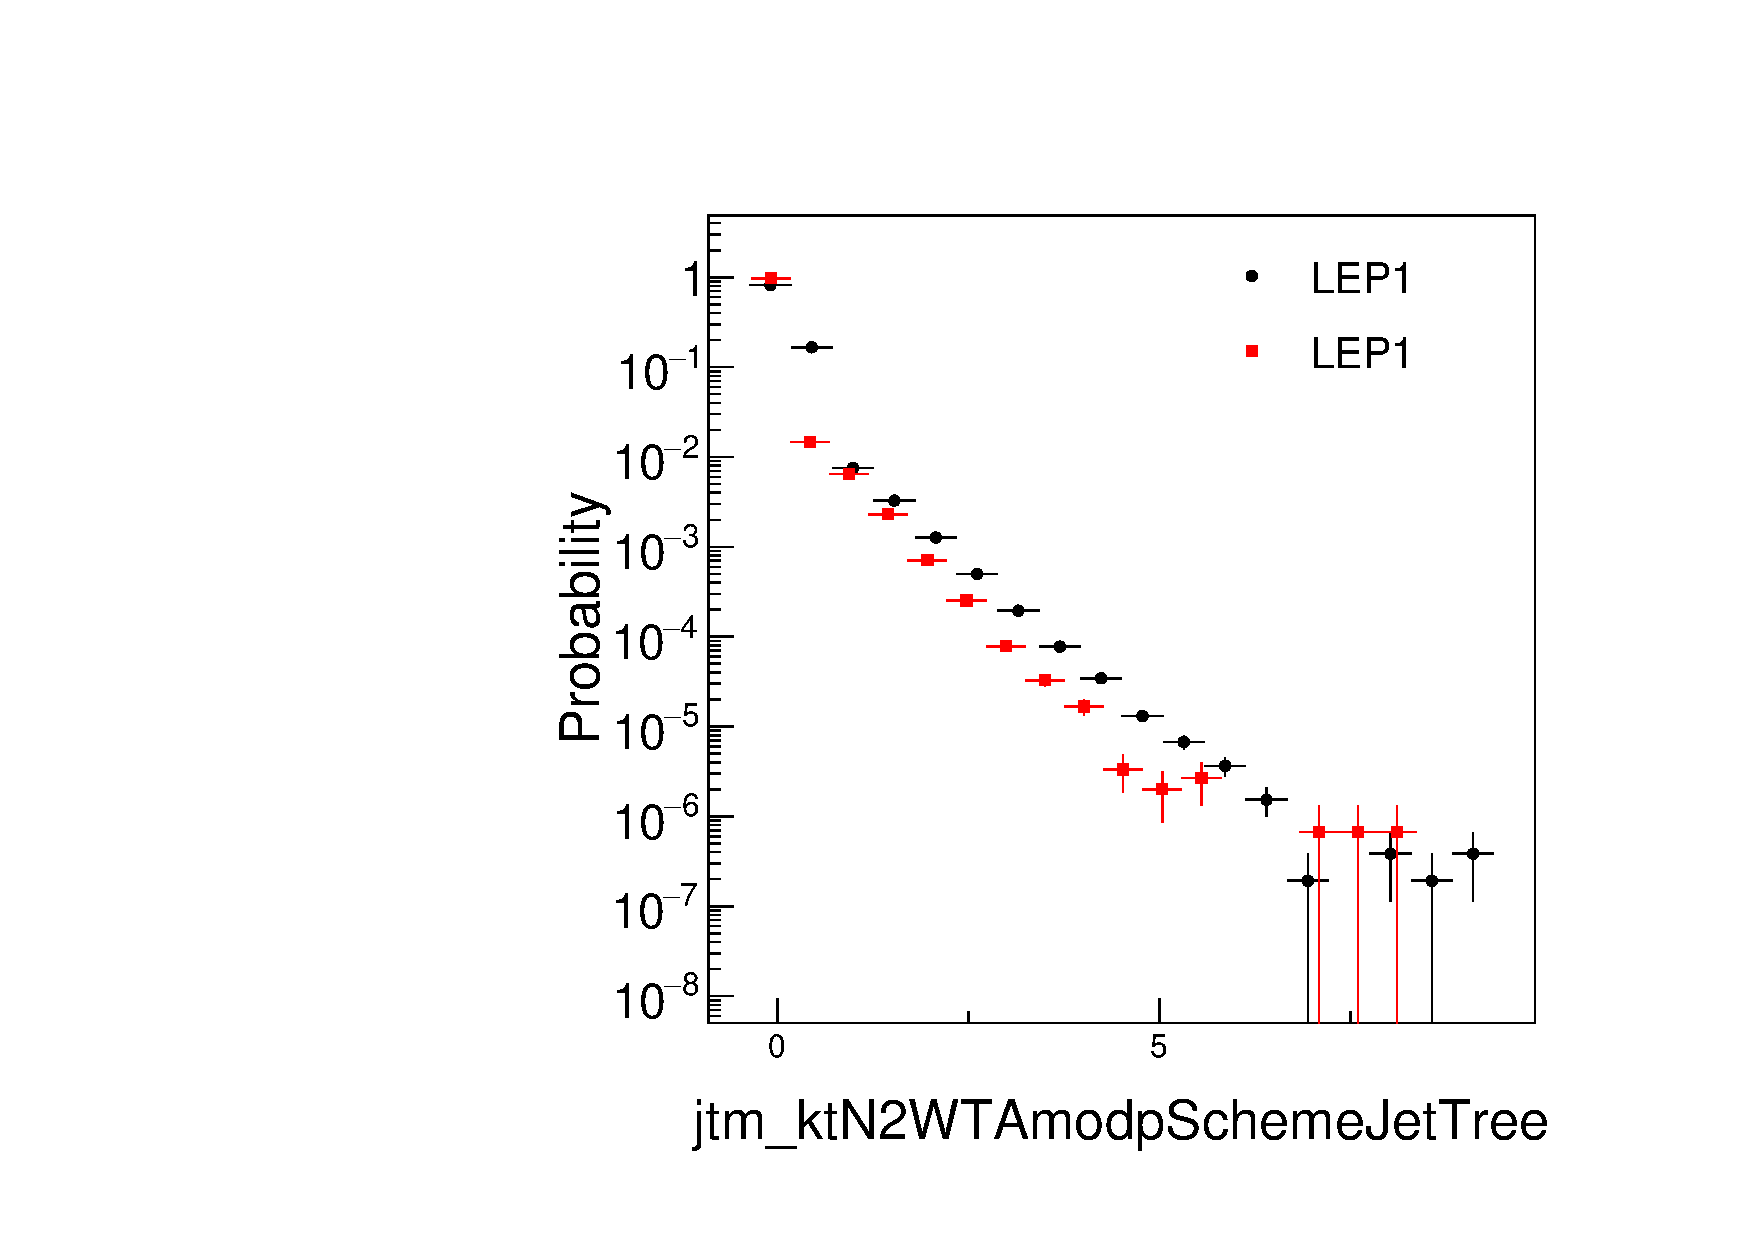
\includegraphics[width=.25\textwidth]{images/DQC/LEP1/jtm_ktN2WTAmodpSchemeJetTree.pdf}}\hfill
\subfloat{\label{sfig:h}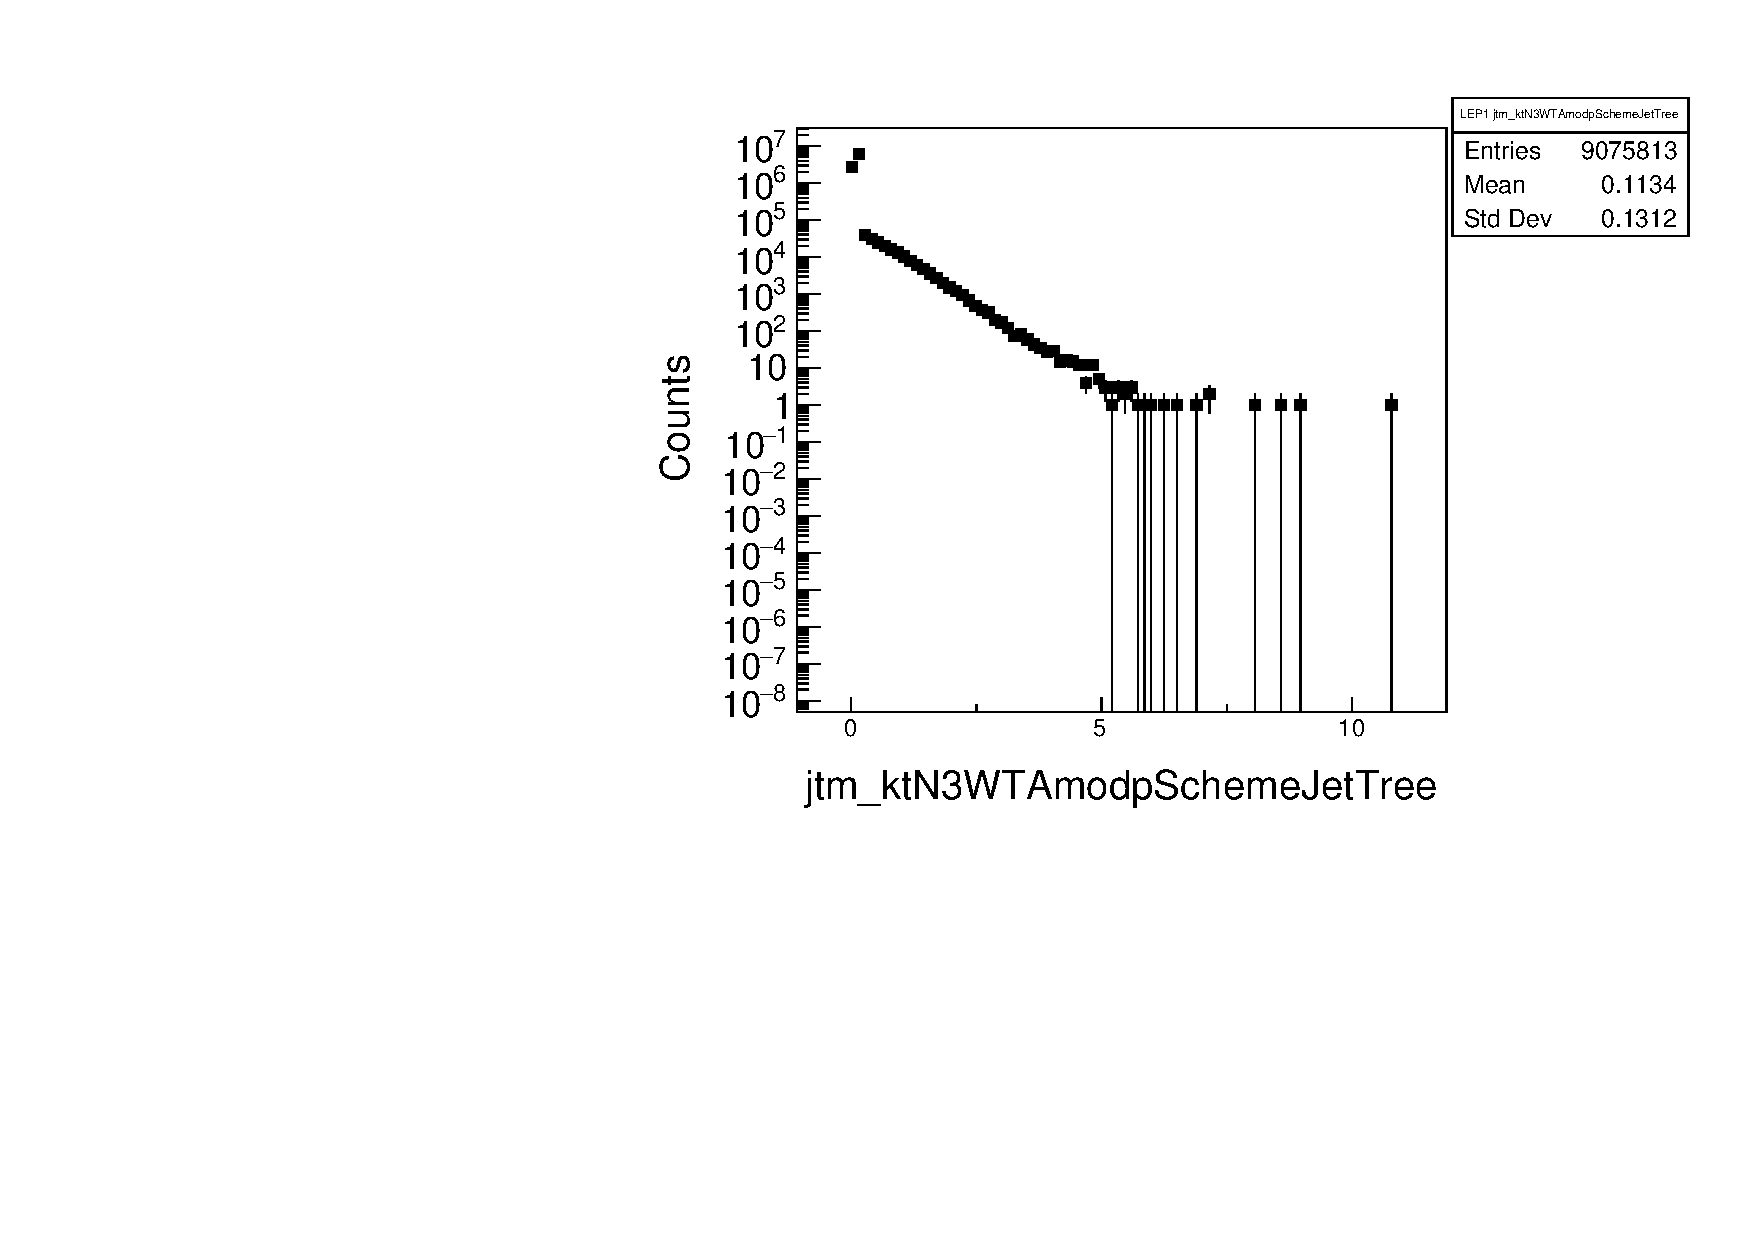
\includegraphics[width=.25\textwidth]{images/DQC/LEP1/jtm_ktN3WTAmodpSchemeJetTree.pdf}}\hfill
\caption{LEP1 Jet mass distributions. Top row: anti-$k_t$, left to right: $R=0.4$, $E$ scheme; $R=0.8$, $E$ scheme; $R=0.4$, WTA mod p scheme; $R=0.8$, WTA mod p scheme. Bottom row: $k_t$, left to right: $N=2$, $E$ scheme; $N=3$, $E$ scheme; $N=2$, WTA mod p scheme; $N=3$; WTA mod p scheme.}  
\end{figure}

\begin{figure}[H]
\centering
\subfloat{\label{sfig:a}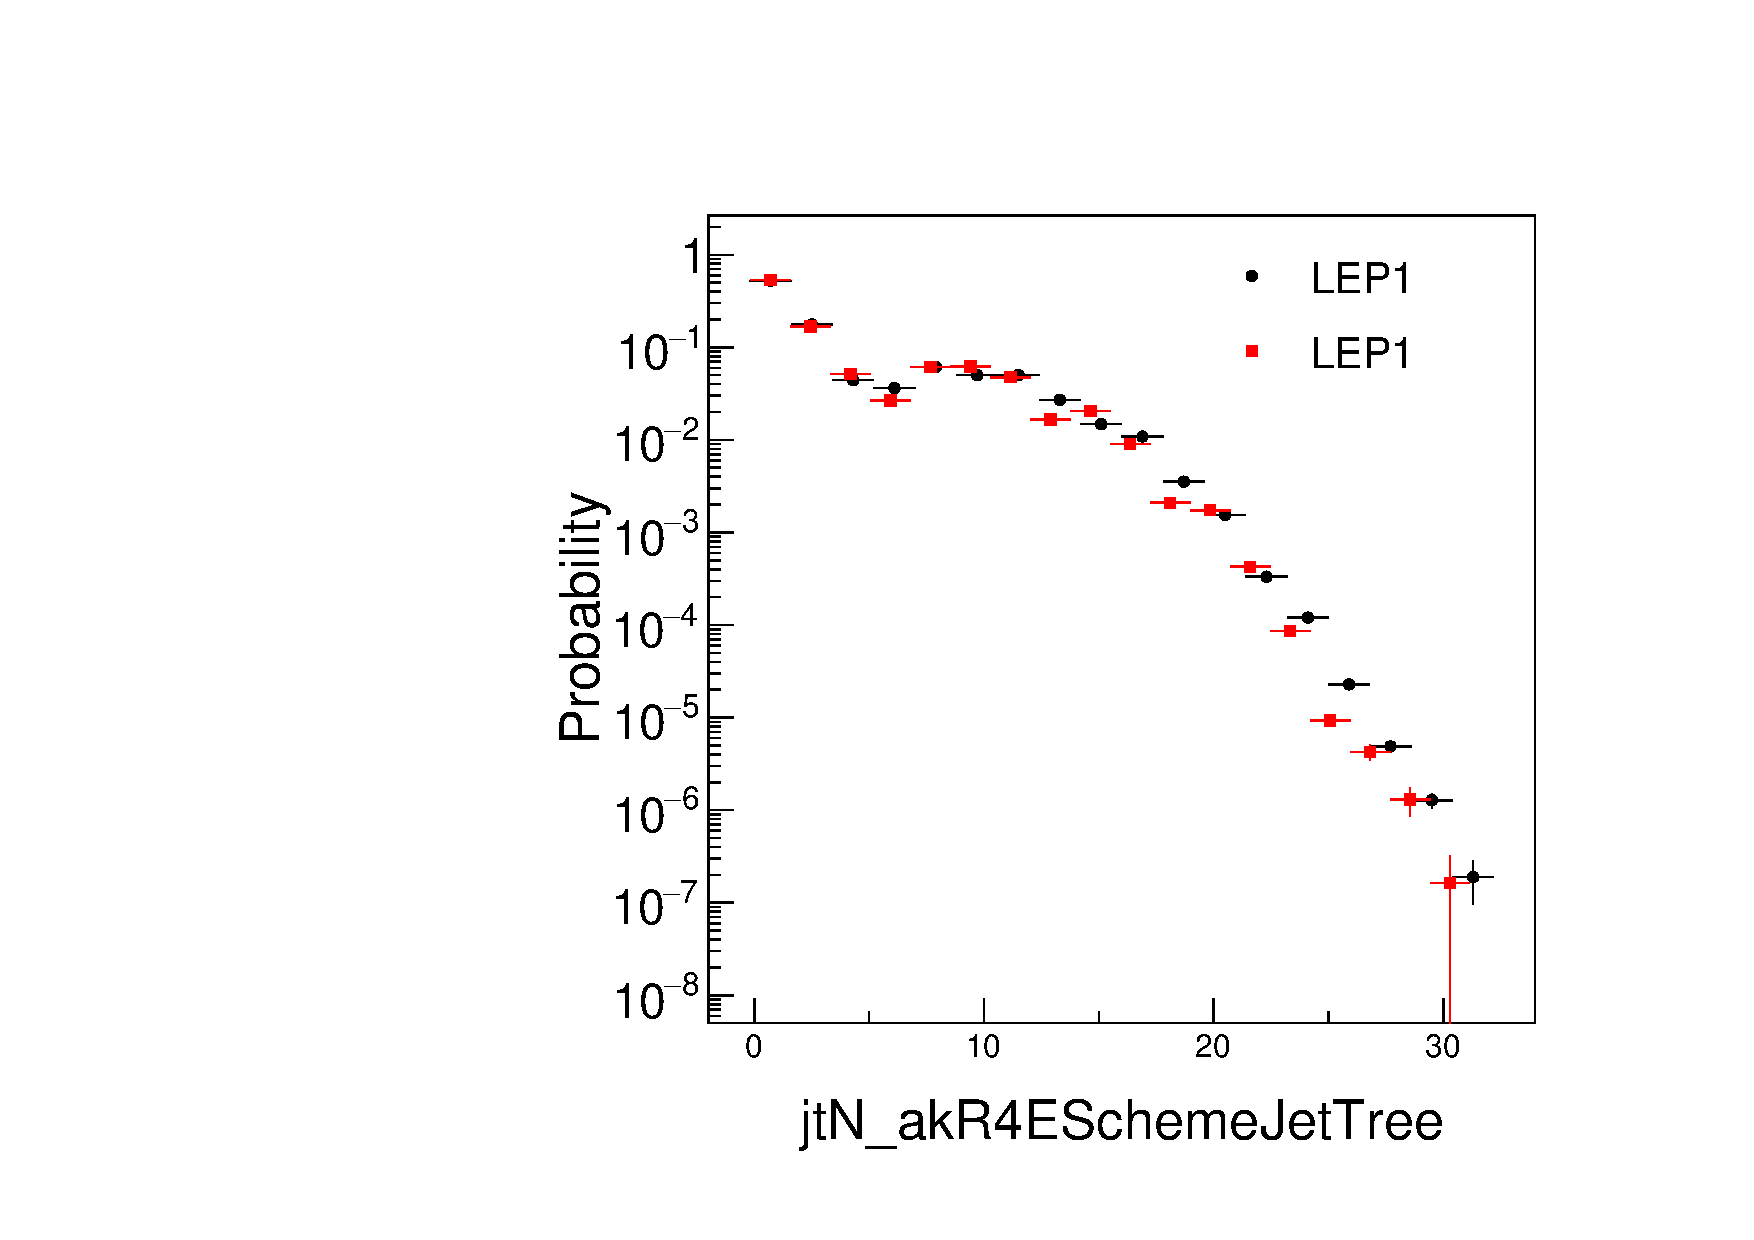
\includegraphics[width=.25\textwidth]{images/DQC/LEP1/jtN_akR4ESchemeJetTree.pdf}}\hfill
\subfloat{\label{sfig:b}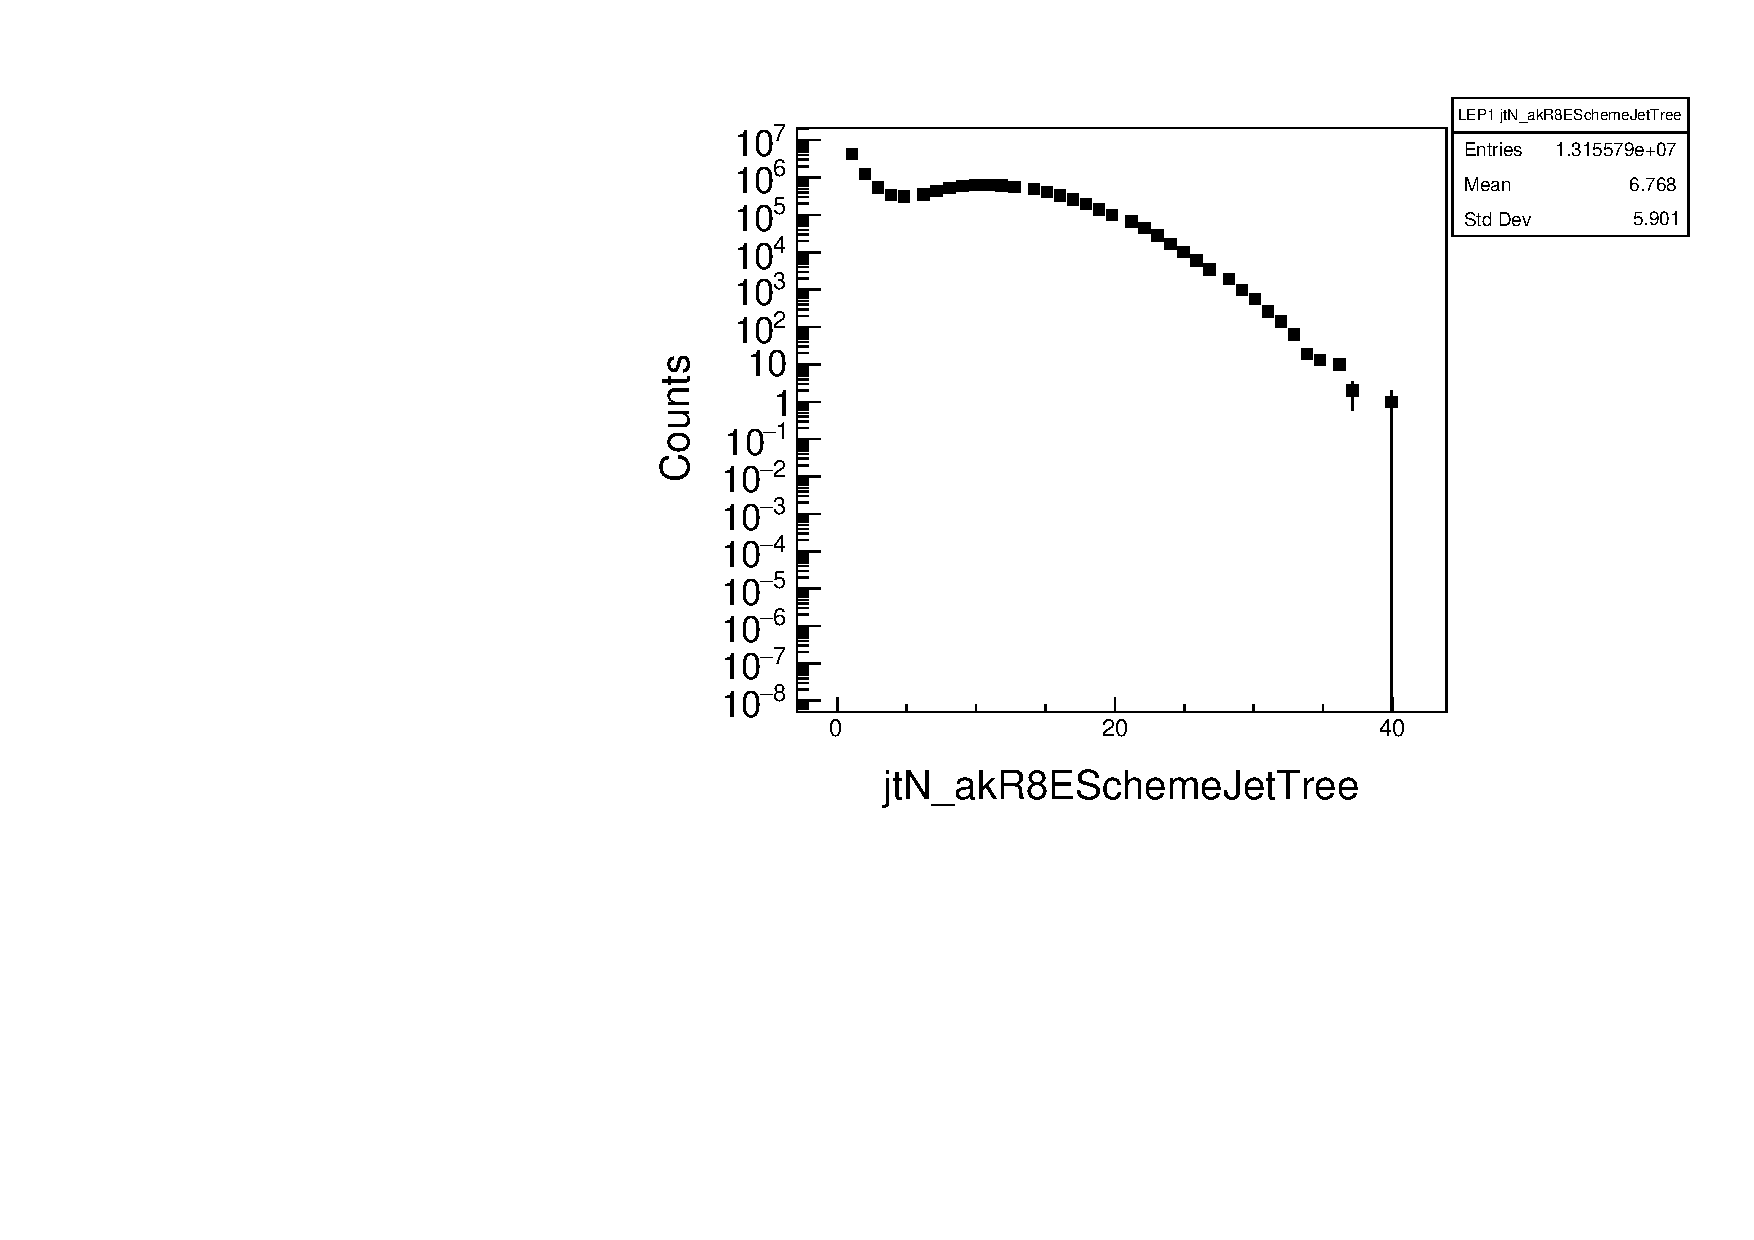
\includegraphics[width=.25\textwidth]{images/DQC/LEP1/jtN_akR8ESchemeJetTree.pdf}}\hfill
\subfloat{\label{sfig:c}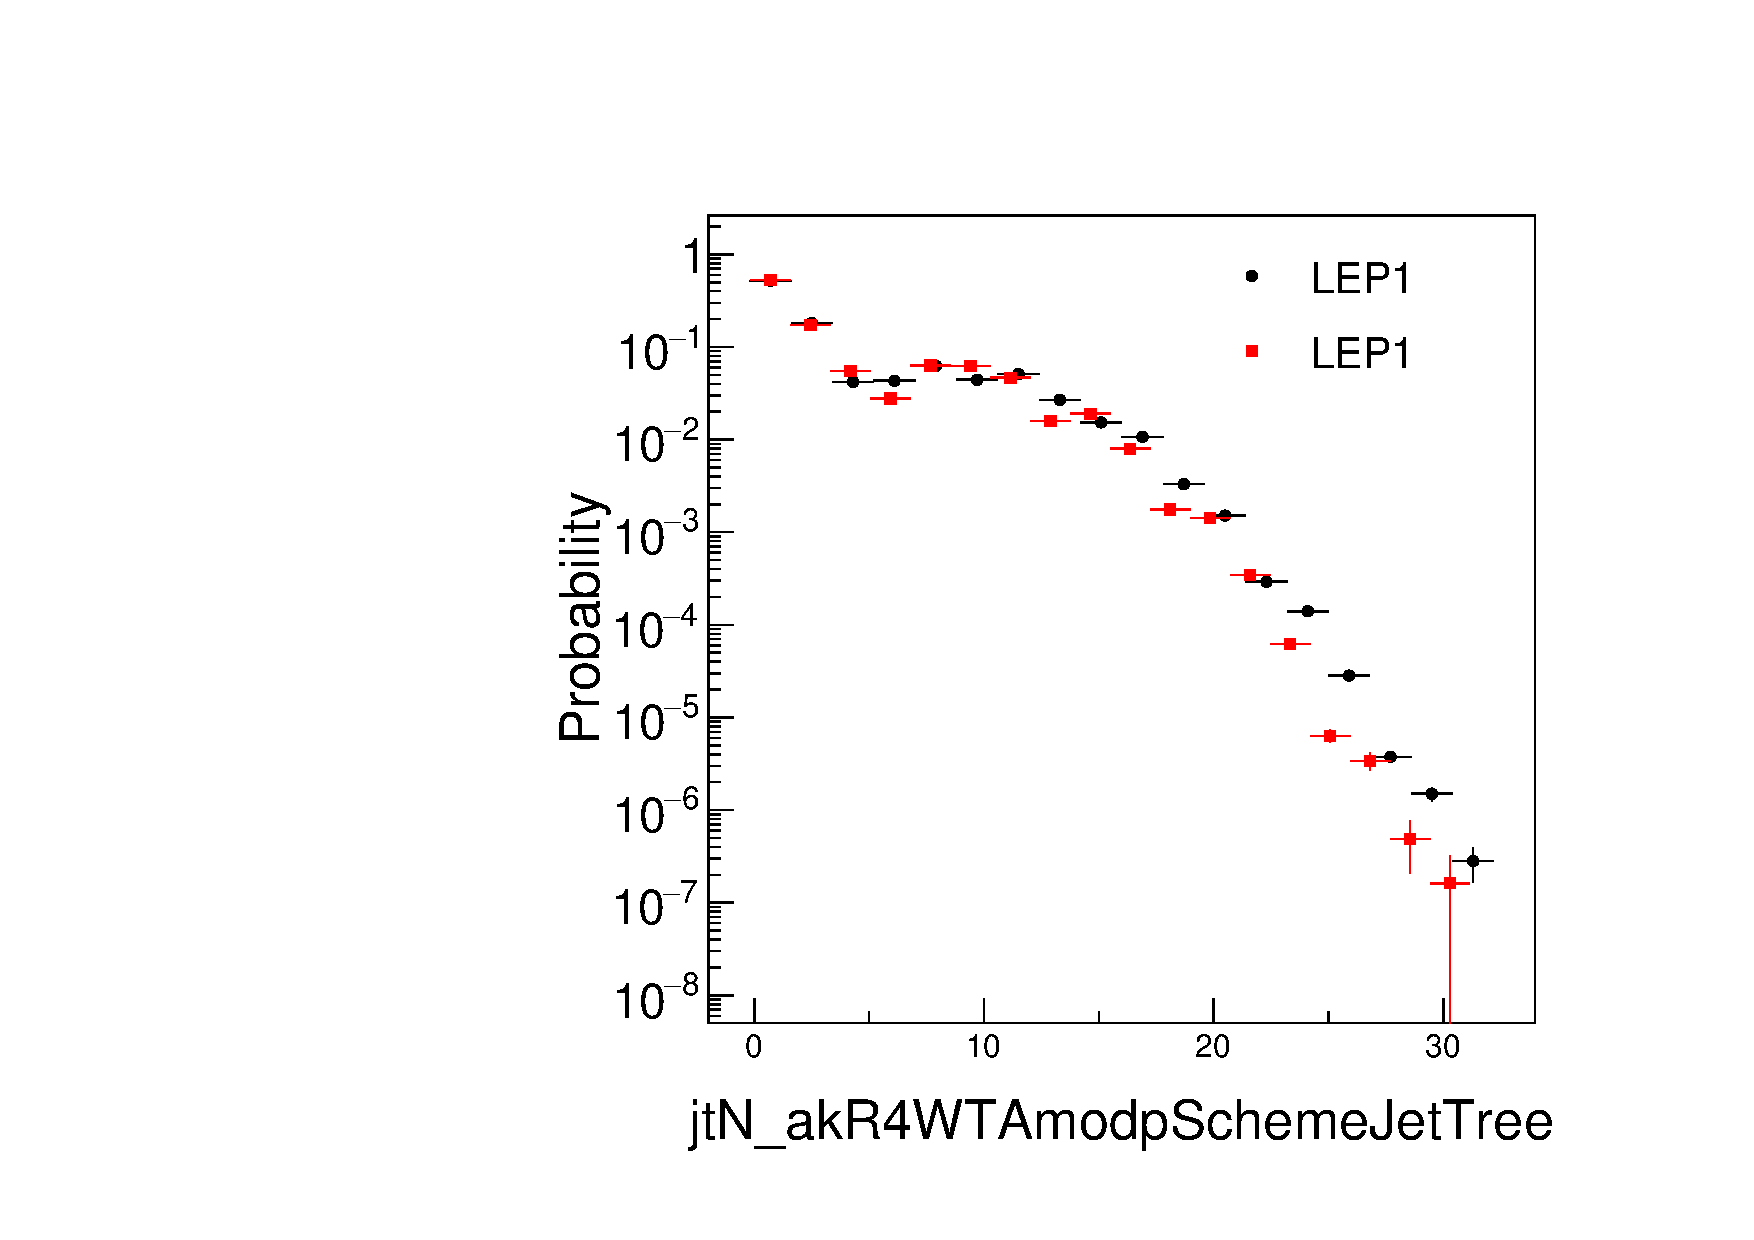
\includegraphics[width=.25\textwidth]{images/DQC/LEP1/jtN_akR4WTAmodpSchemeJetTree.pdf}}\hfill
\subfloat{\label{sfig:d}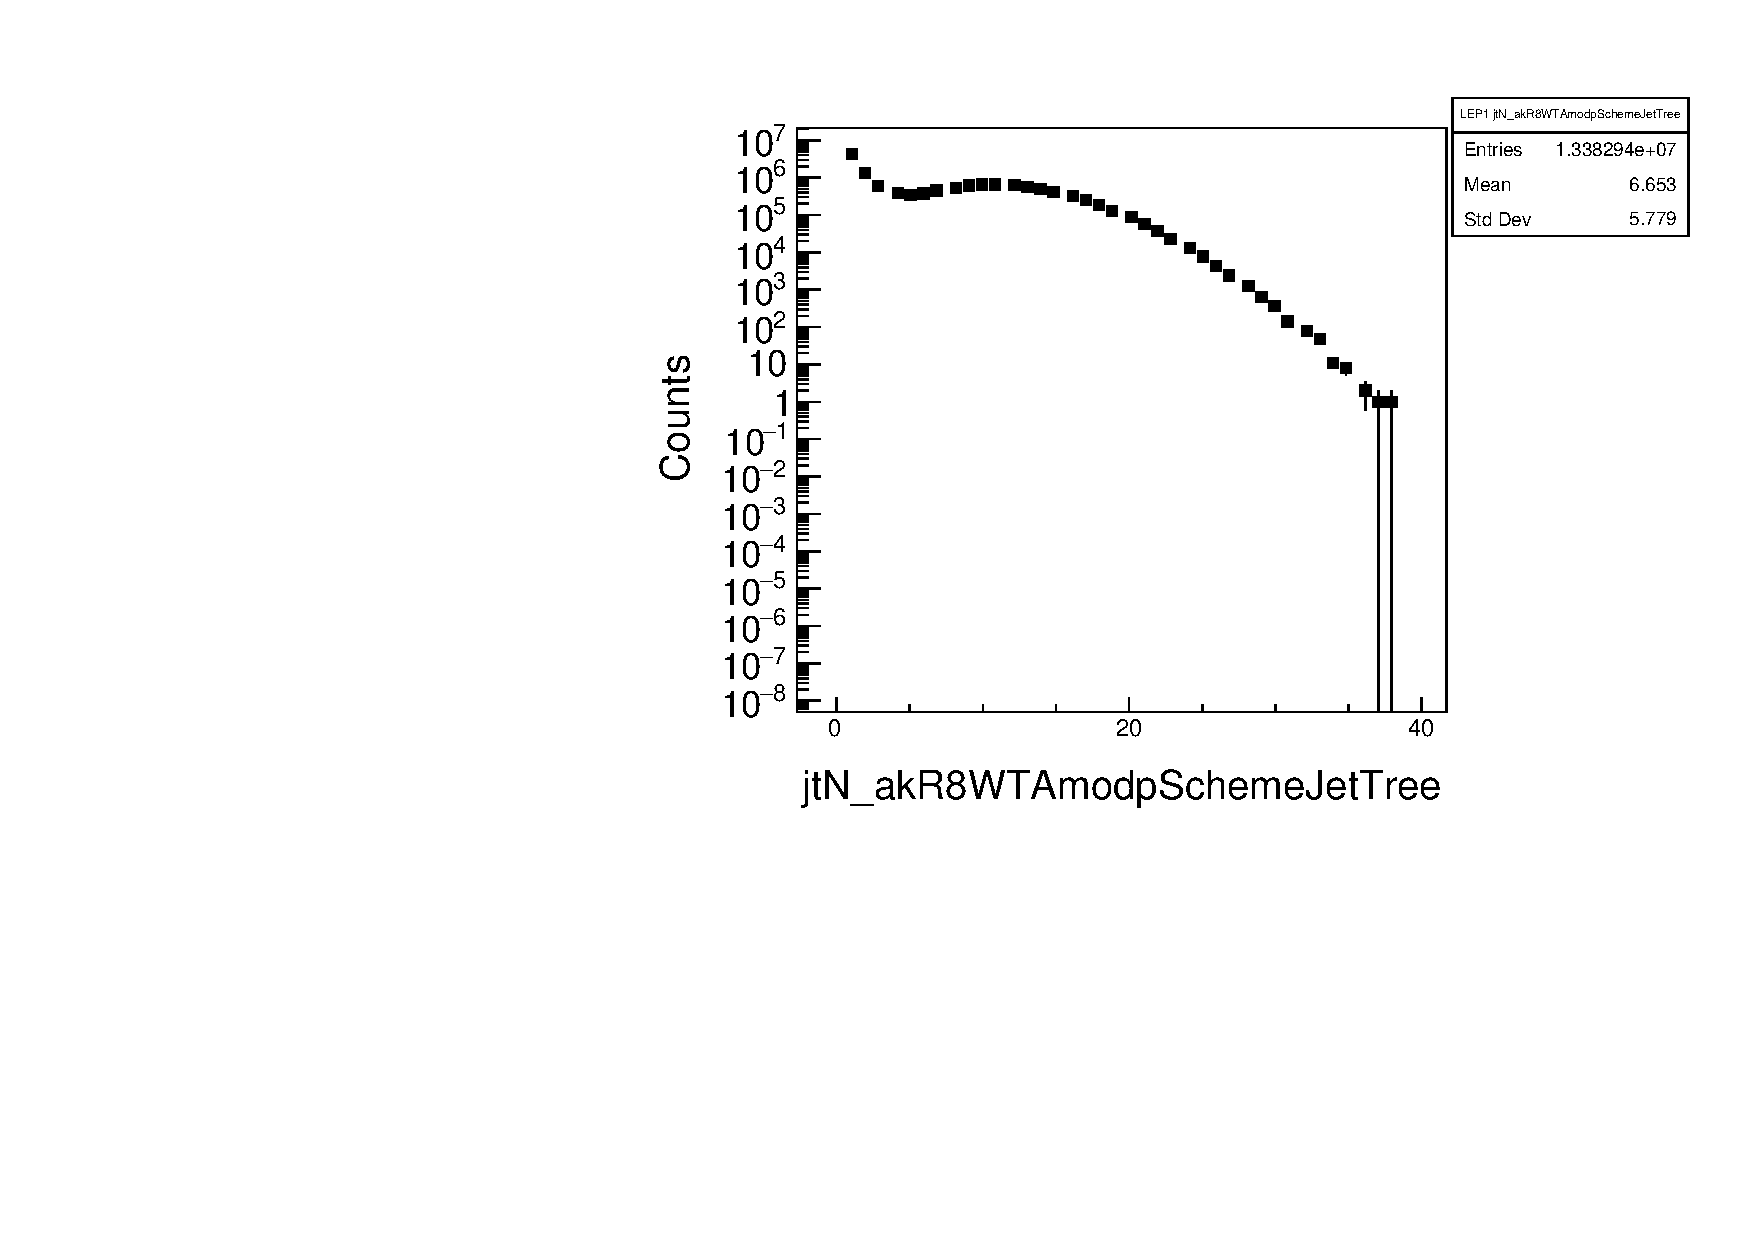
\includegraphics[width=.25\textwidth]{images/DQC/LEP1/jtN_akR8WTAmodpSchemeJetTree.pdf}}\hfill %row end
\subfloat{\label{sfig:e}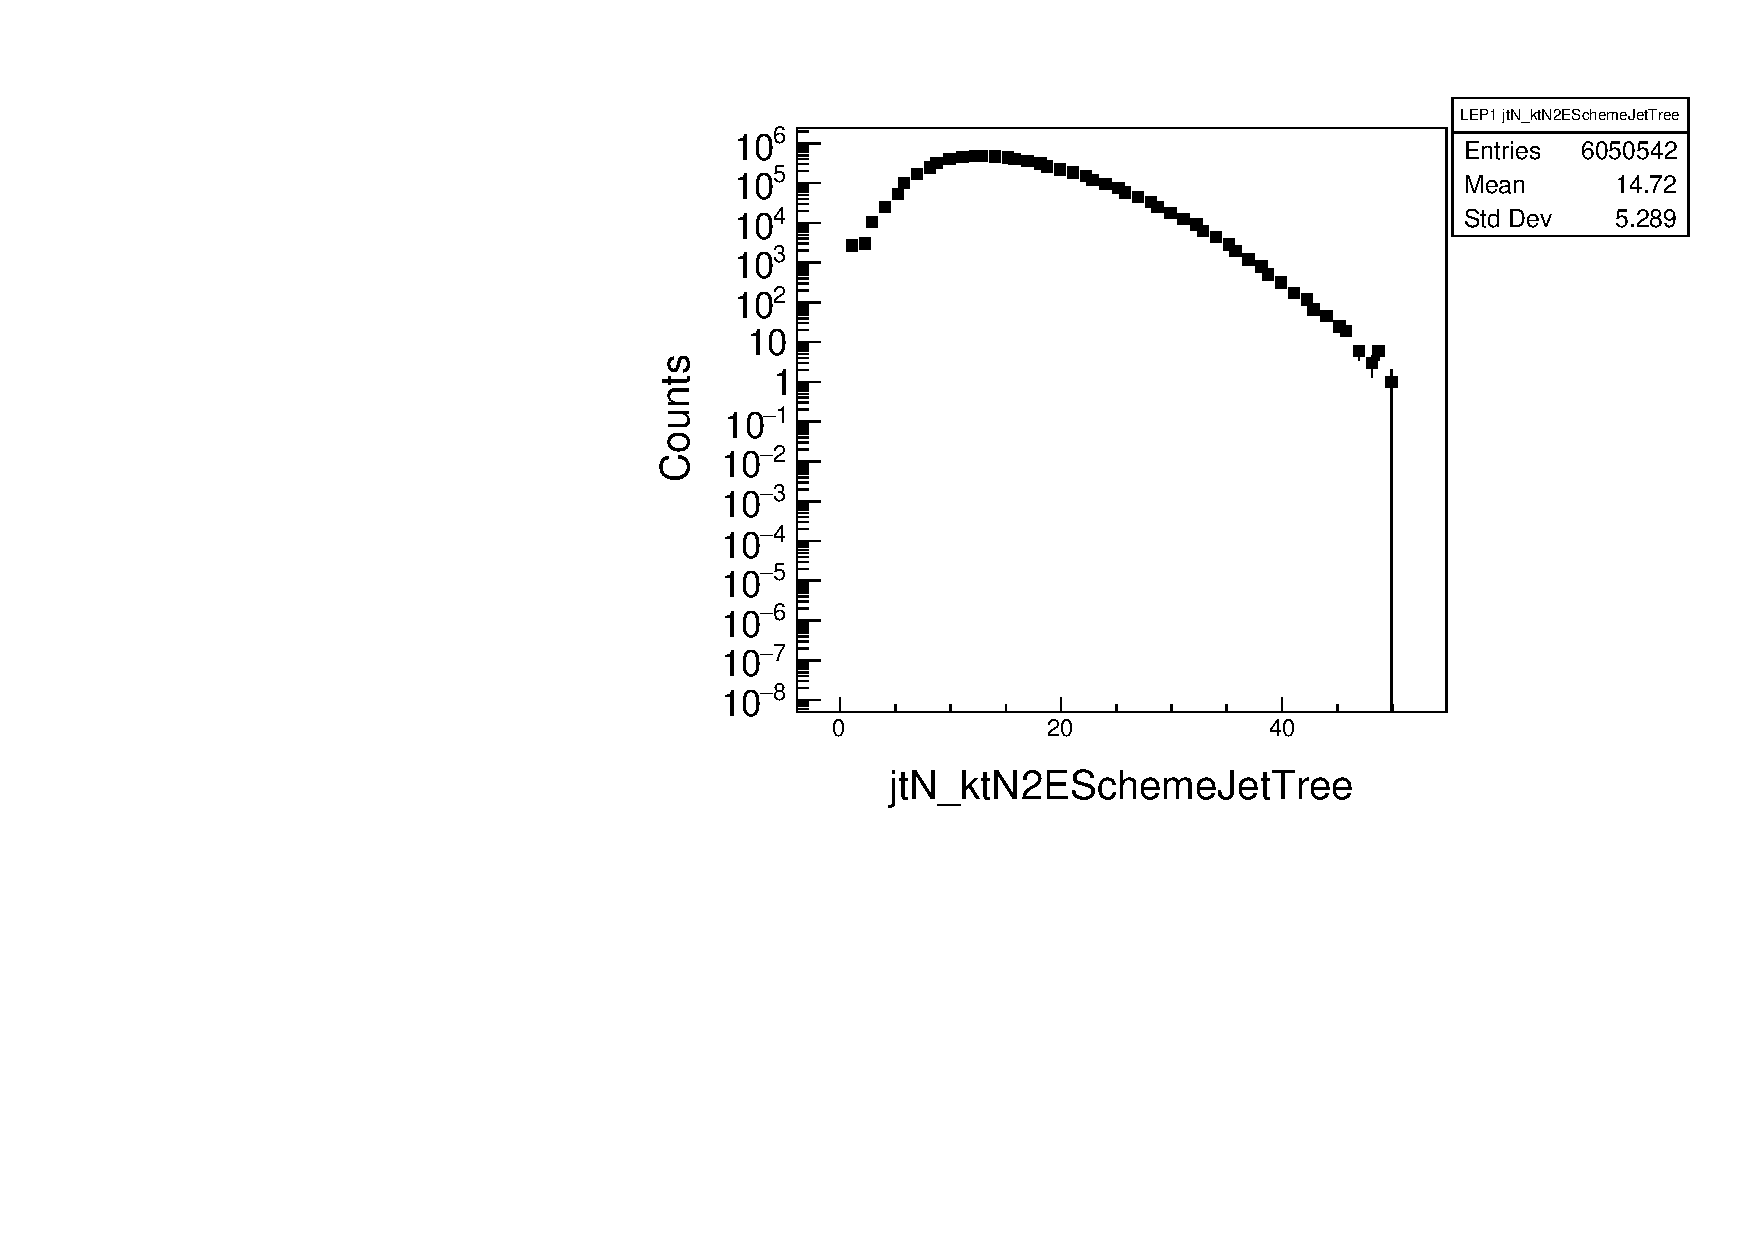
\includegraphics[width=.25\textwidth]{images/DQC/LEP1/jtN_ktN2ESchemeJetTree.pdf}}\hfill
\subfloat{\label{sfig:f}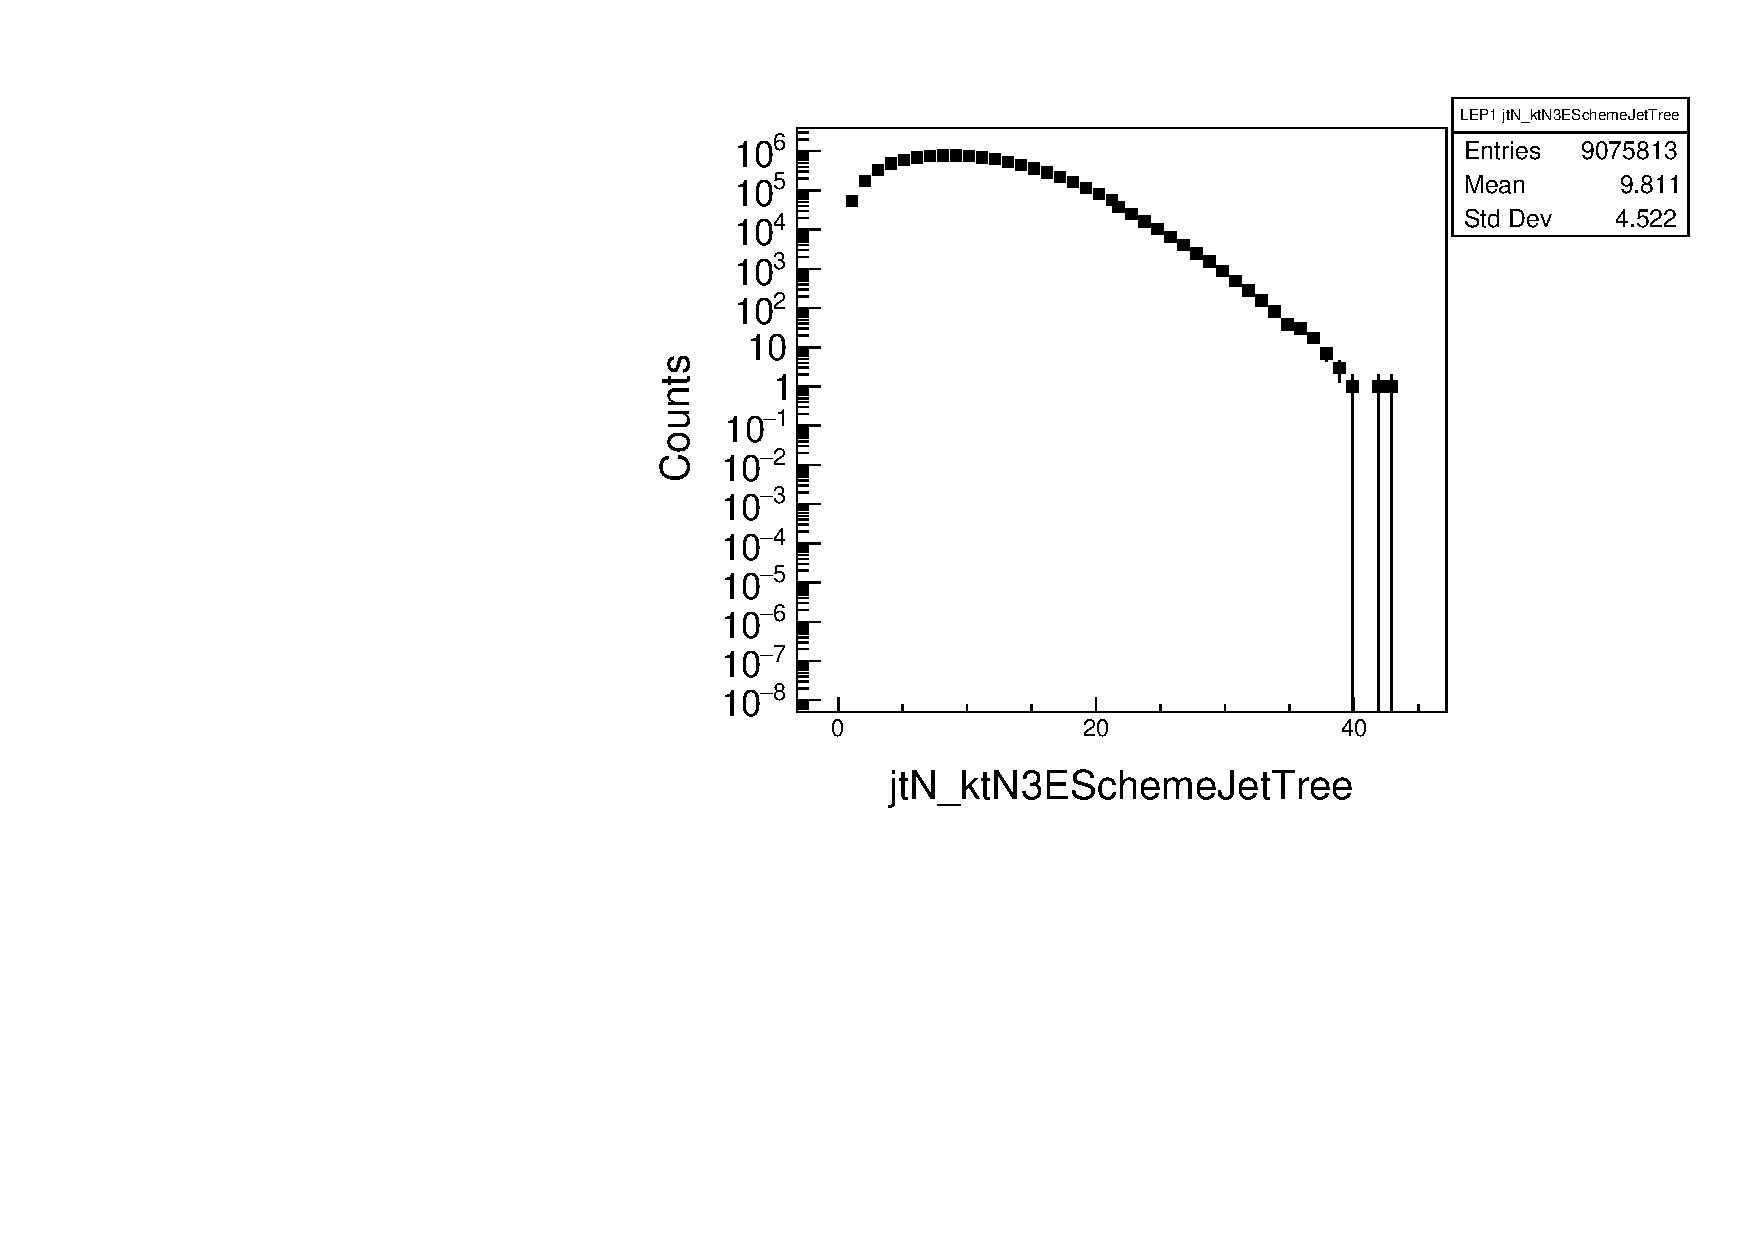
\includegraphics[width=.25\textwidth]{images/DQC/LEP1/jtN_ktN3ESchemeJetTree.pdf}}\hfill
\subfloat{\label{sfig:g}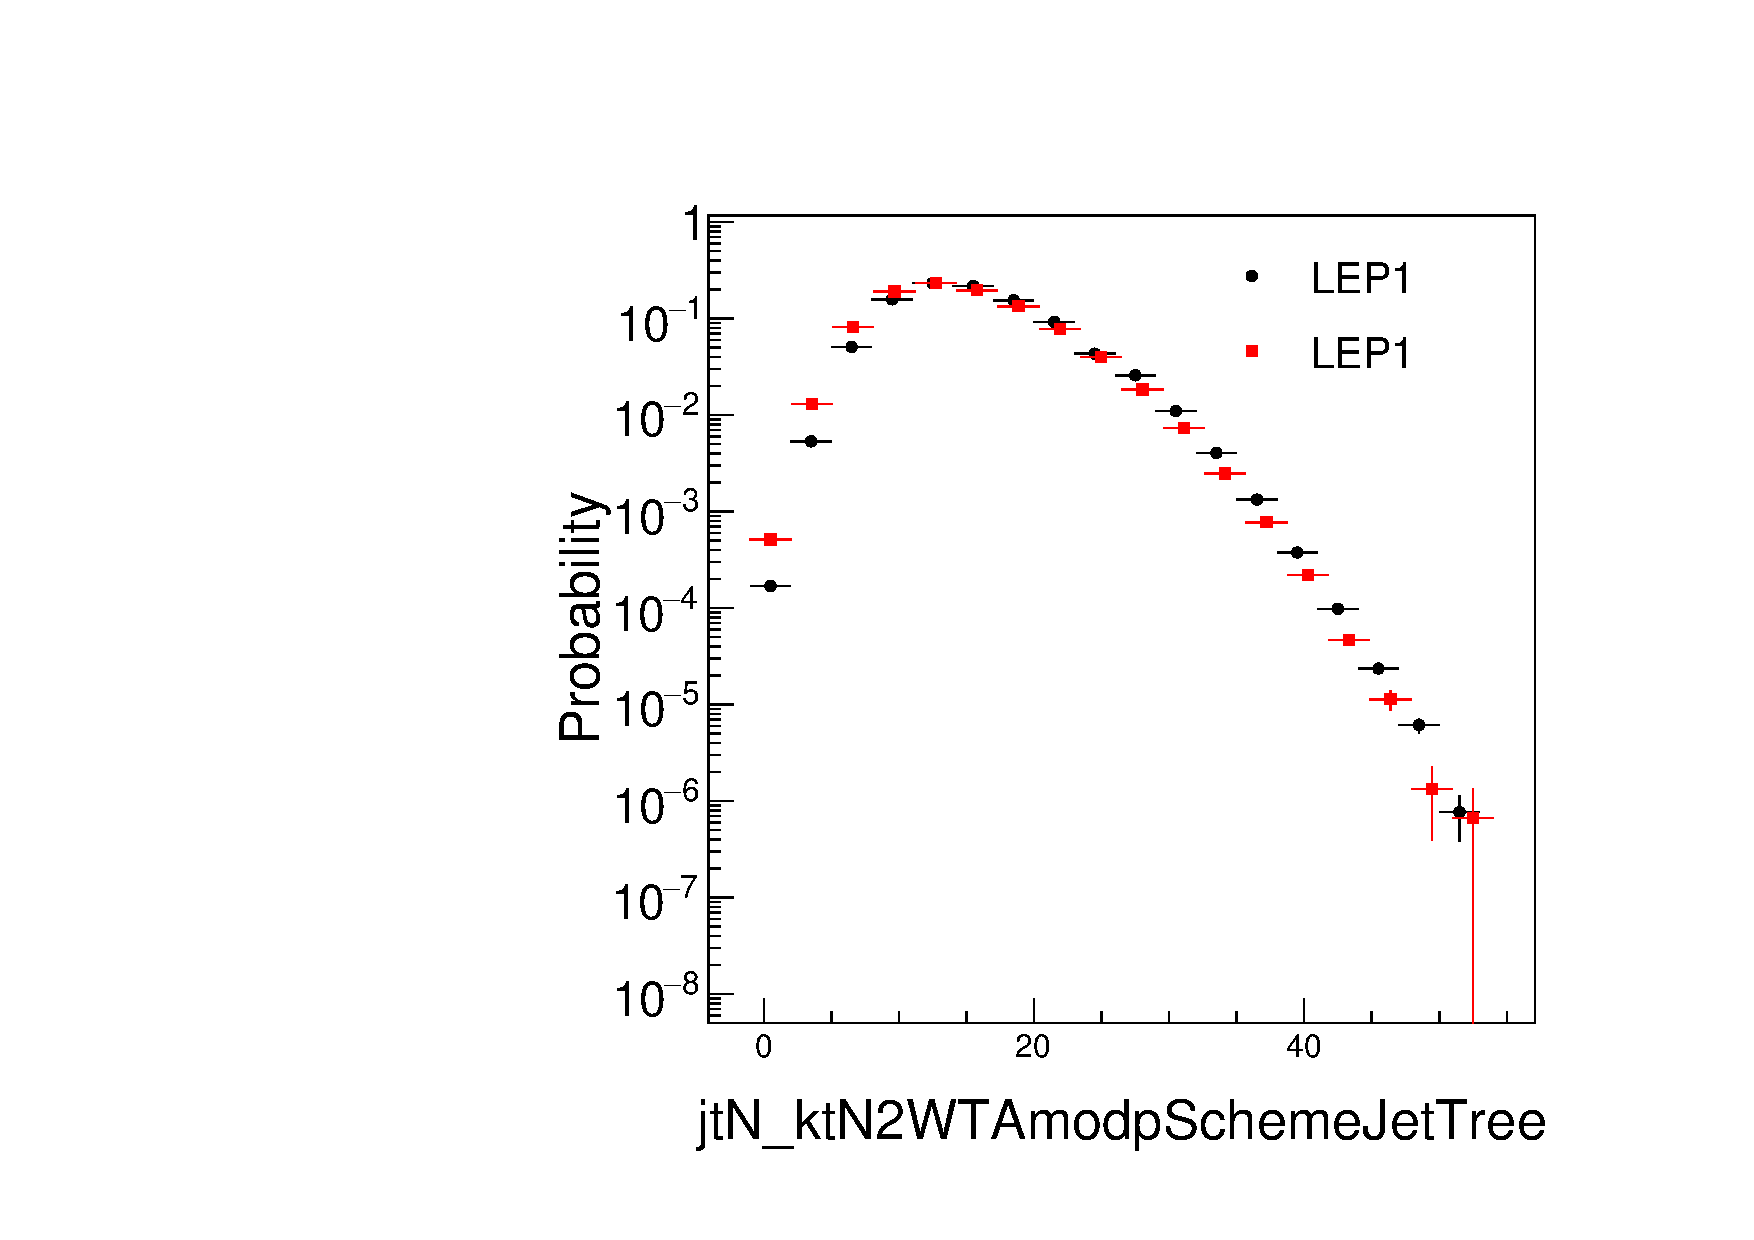
\includegraphics[width=.25\textwidth]{images/DQC/LEP1/jtN_ktN2WTAmodpSchemeJetTree.pdf}}\hfill
\subfloat{\label{sfig:h}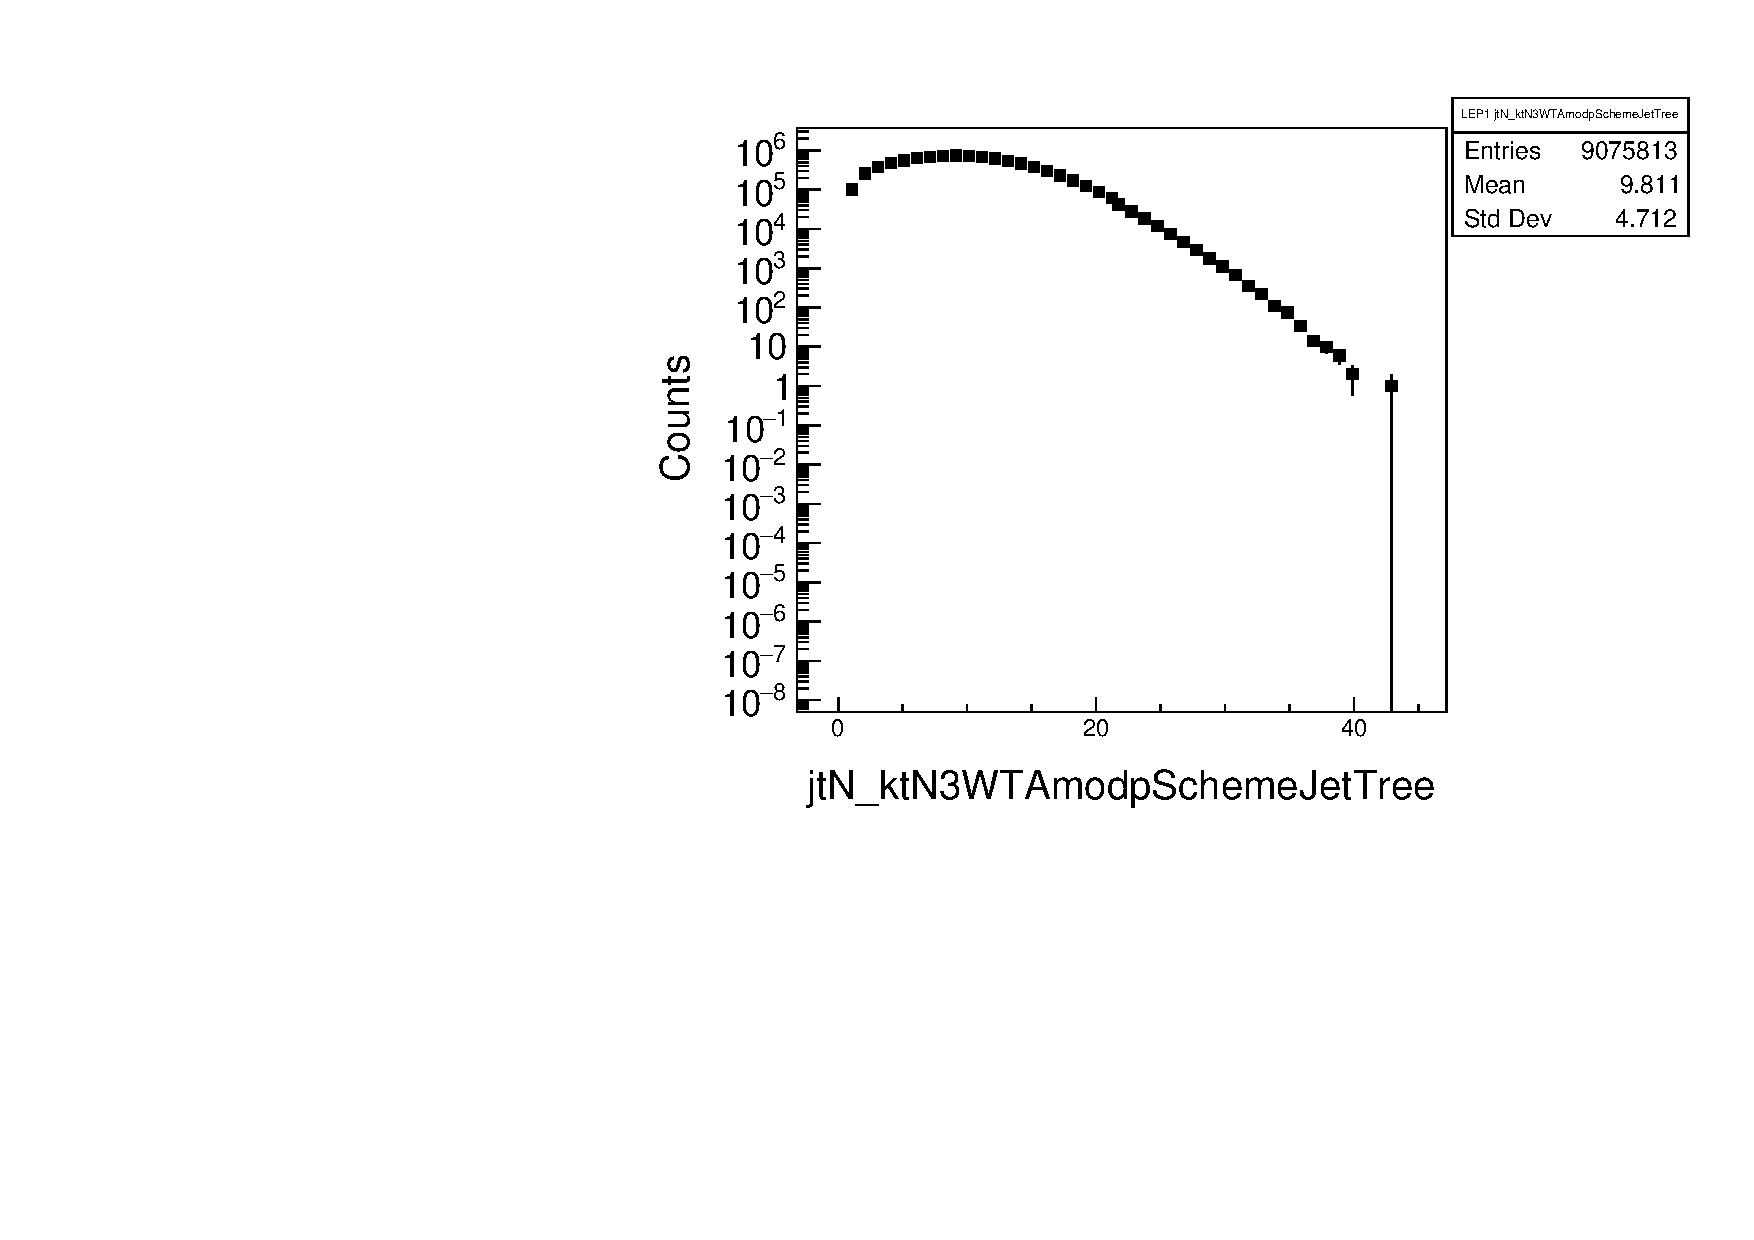
\includegraphics[width=.25\textwidth]{images/DQC/LEP1/jtN_ktN3WTAmodpSchemeJetTree.pdf}}\hfill
\caption{LEP1 Jet $N$ distributions. Top row: anti-$k_t$, left to right: $R=0.4$, $E$ scheme; $R=0.8$, $E$ scheme; $R=0.4$, WTA mod p scheme; $R=0.8$, WTA mod p scheme. Bottom row: $k_t$, left to right: $N=2$, $E$ scheme; $N=3$, $E$ scheme; $N=2$, WTA mod p scheme; $N=3$; WTA mod p scheme.}  
\end{figure} 

\begin{figure}[H]
\centering
\subfloat{\label{sfig:a}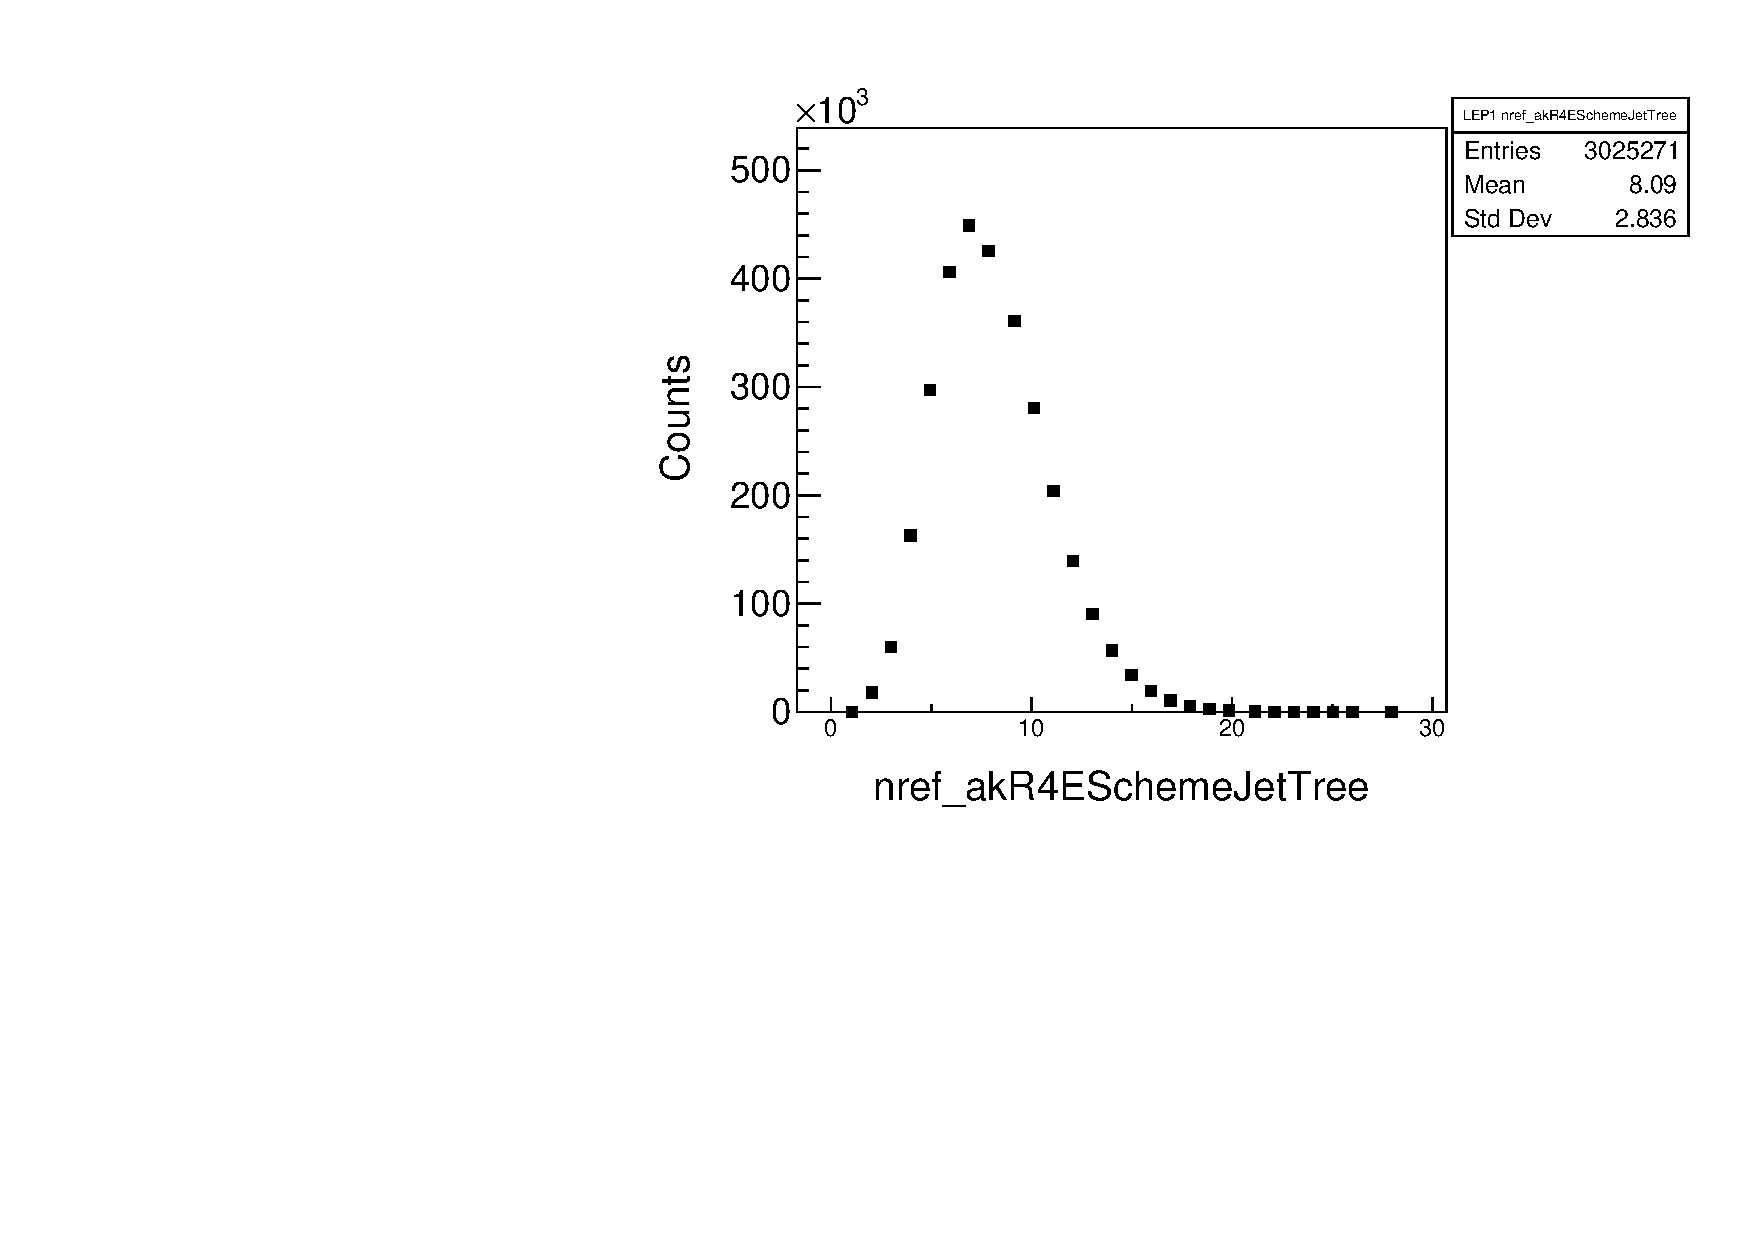
\includegraphics[width=.25\textwidth]{images/DQC/LEP1/nref_akR4ESchemeJetTree.pdf}}\hfill
\subfloat{\label{sfig:b}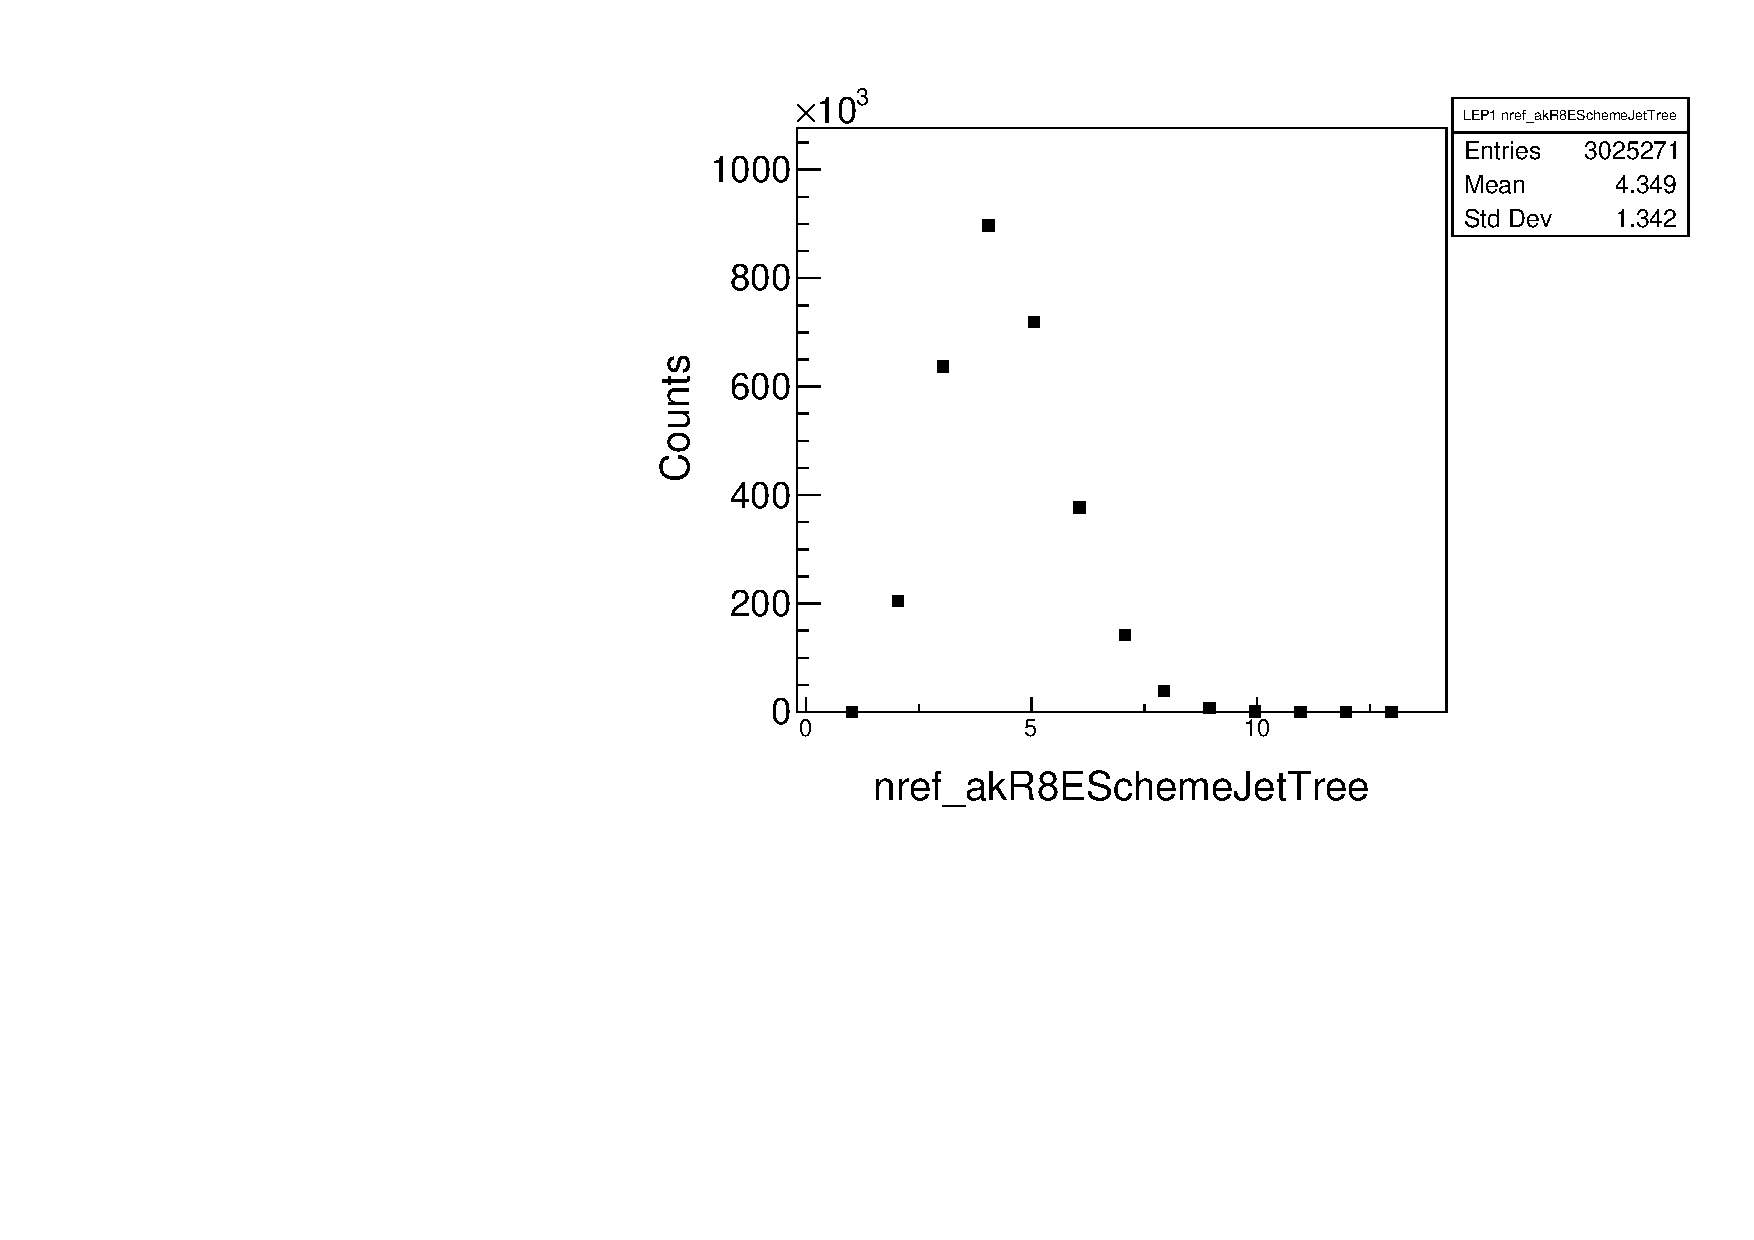
\includegraphics[width=.25\textwidth]{images/DQC/LEP1/nref_akR8ESchemeJetTree.pdf}}\hfill
\subfloat{\label{sfig:c}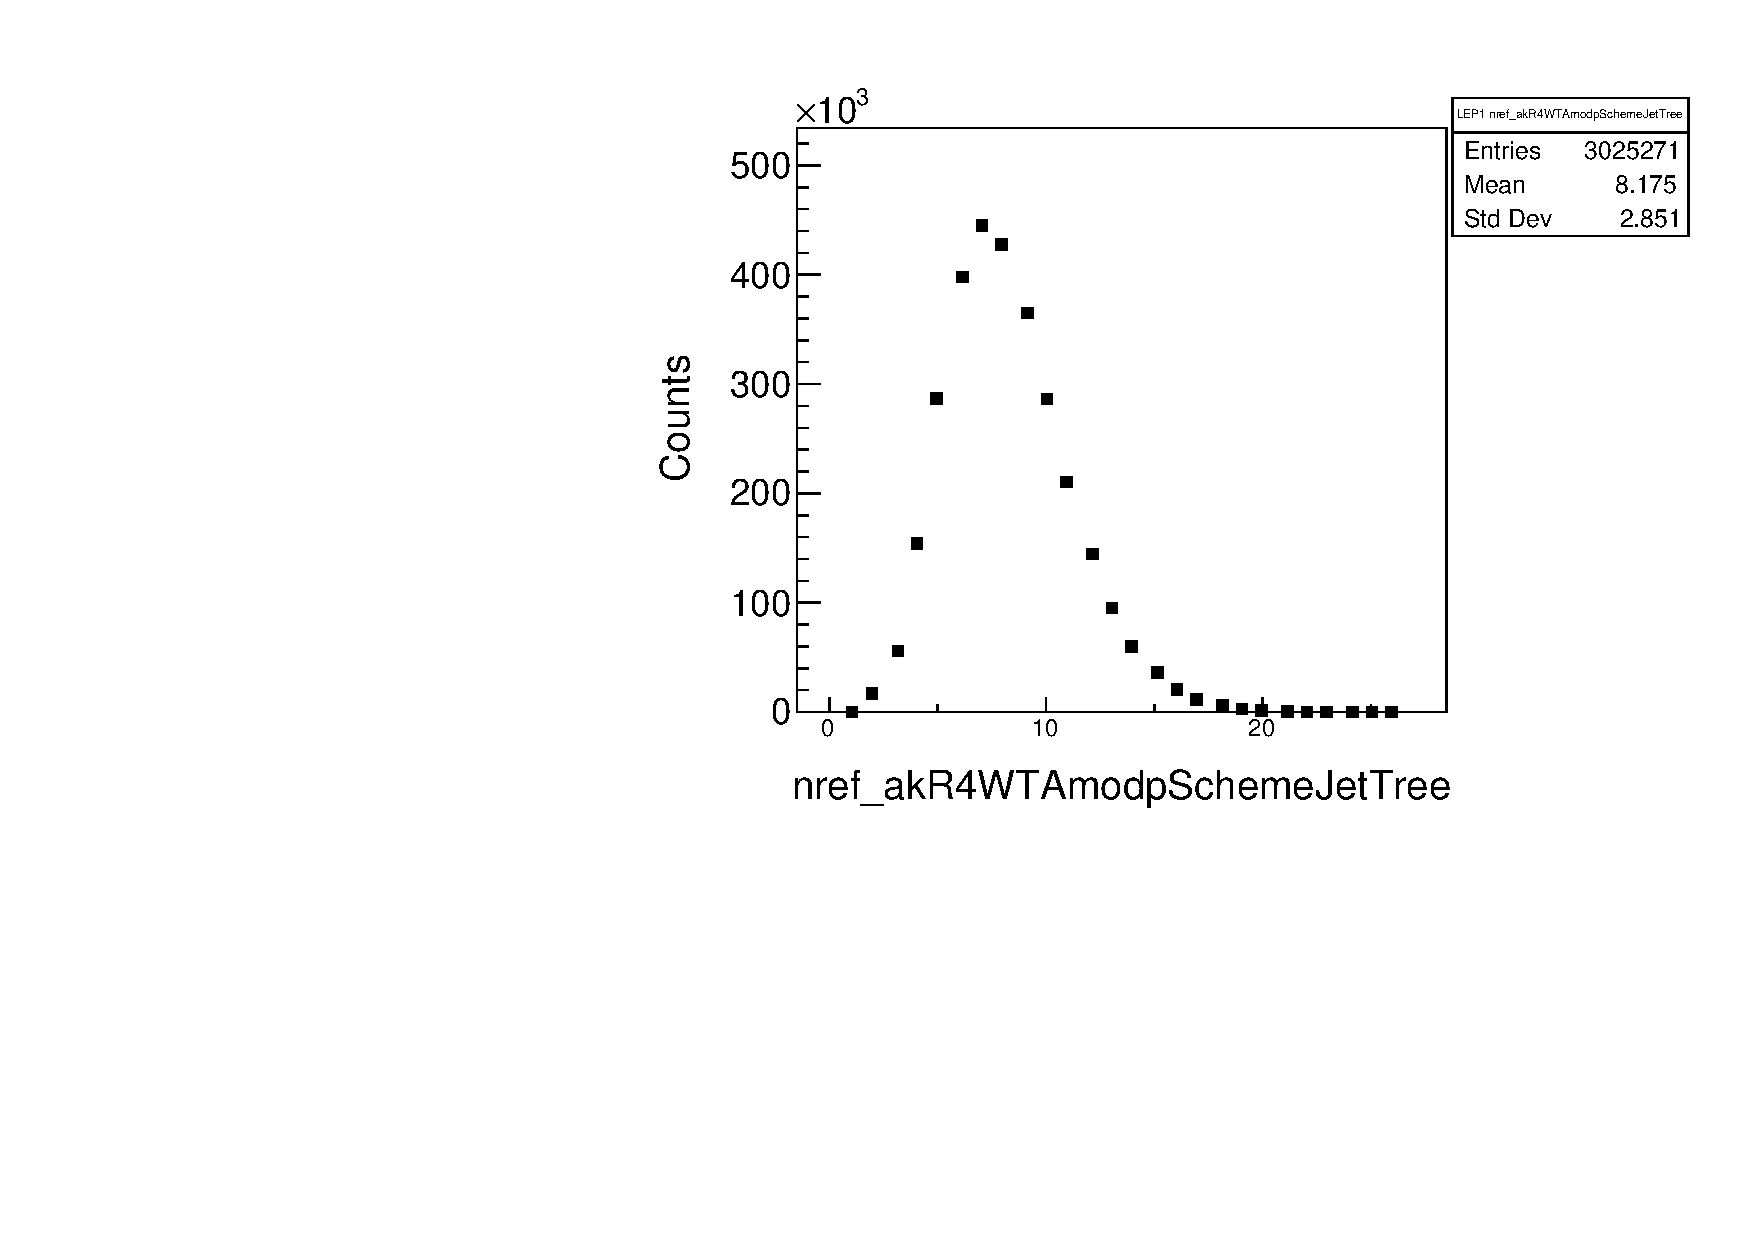
\includegraphics[width=.25\textwidth]{images/DQC/LEP1/nref_akR4WTAmodpSchemeJetTree.pdf}}\hfill
\subfloat{\label{sfig:d}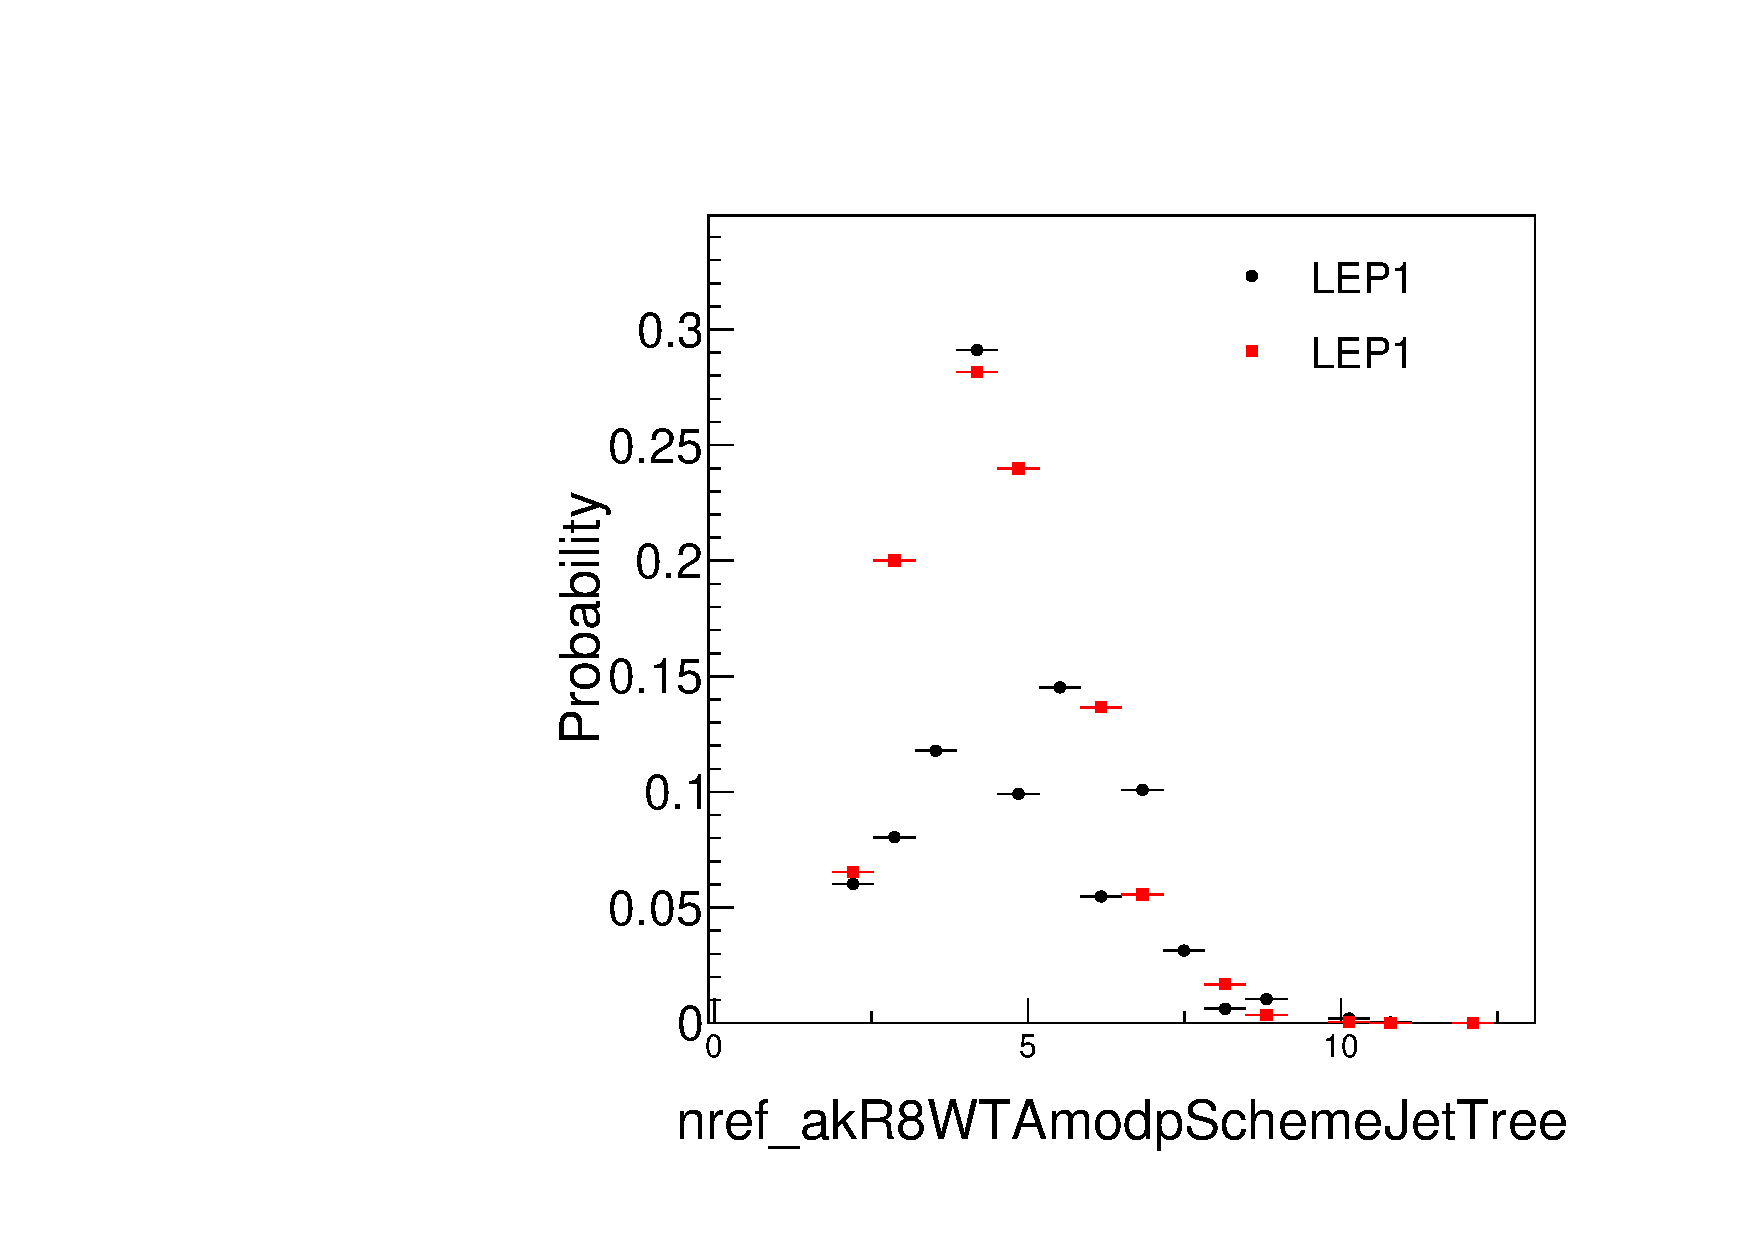
\includegraphics[width=.25\textwidth]{images/DQC/LEP1/nref_akR8WTAmodpSchemeJetTree.pdf}}\hfill %row end
\subfloat{\label{sfig:e}\includegraphics[width=.25\textwidth]{images/DQC/LEP1/nref_ktN2ESchemeJetTree.pdf}}\hfill
\subfloat{\label{sfig:f}\includegraphics[width=.25\textwidth]{images/DQC/LEP1/nref_ktN3ESchemeJetTree.pdf}}\hfill
\subfloat{\label{sfig:g}\includegraphics[width=.25\textwidth]{images/DQC/LEP1/nref_ktN2WTAmodpSchemeJetTree.pdf}}\hfill
\subfloat{\label{sfig:h}\includegraphics[width=.25\textwidth]{images/DQC/LEP1/nref_ktN3WTAmodpSchemeJetTree.pdf}}\hfill
\caption{LEP1 Jet nref distributions. Top row: anti-$k_t$, left to right: $R=0.4$, $E$ scheme; $R=0.8$, $E$ scheme; $R=0.4$, WTA mod p scheme; $R=0.8$, WTA mod p scheme. Bottom row: $k_t$, left to right: $N=2$, $E$ scheme; $N=3$, $E$ scheme; $N=2$, WTA mod p scheme; $N=3$; WTA mod p scheme.}  
\end{figure}

\begin{figure}[H]
\centering
\subfloat{\label{sfig:a}\includegraphics[width=.33\textwidth]{images/DQC/LEP1/eta.pdf}}\hfill
\subfloat{\label{sfig:b}\includegraphics[width=.33\textwidth]{images/DQC/LEP1/eta_wrtThr.pdf}}\hfill
\subfloat{\label{sfig:c}\includegraphics[width=.33\textwidth]{images/DQC/LEP1/eta_wrtChThr.pdf}}\hfill
\caption{LEP1 $\eta$ distributions. Left to right: $\eta$; $\eta$ with respect to thrust axis; $\eta$ with respect to charged thrust axis.}
\end{figure}

\begin{figure}[H]
\centering
\subfloat{\label{sfig:a}\includegraphics[width=.33\textwidth]{images/DQC/LEP1/phi.pdf}}\hfill
\subfloat{\label{sfig:b}\includegraphics[width=.33\textwidth]{images/DQC/LEP1/phi_wrtThr.pdf}}\hfill
\subfloat{\label{sfig:c}\includegraphics[width=.33\textwidth]{images/DQC/LEP1/phi_wrtChThr.pdf}}\hfill
\caption{LEP1 $\phi$ distributions. Left to right: $\phi$; $\phi$ with respect to thrust axis; $\phi$ with respect to charged thrust axis.}
\end{figure}

\begin{figure}[H]
\centering
\subfloat{\label{sfig:a}\includegraphics[width=.33\textwidth]{images/DQC/LEP1/pt.pdf}}\hfill
\subfloat{\label{sfig:b}\includegraphics[width=.33\textwidth]{images/DQC/LEP1/pt_wrtThr.pdf}}\hfill
\subfloat{\label{sfig:c}\includegraphics[width=.33\textwidth]{images/DQC/LEP1/pt_wrtChThr.pdf}}\hfill
\caption{LEP1 $p_t$ distributions. Left to right: $p_t$; $p_t$ with respect to thrust axis; $p_t$ with respect to charged thrust axis.}
\end{figure}

\begin{figure}[H]
\centering
\subfloat{\label{sfig:a}\includegraphics[width=.33\textwidth]{images/DQC/LEP1/theta.pdf}}\hfill
\subfloat{\label{sfig:b}\includegraphics[width=.33\textwidth]{images/DQC/LEP1/theta_wrtThr.pdf}}\hfill
\subfloat{\label{sfig:c}\includegraphics[width=.33\textwidth]{images/DQC/LEP1/theta_wrtChThr.pdf}}\hfill
\caption{LEP1 $\theta$ distributions. Left to right: $\theta$; $\theta$ with respect to thrust axis; $\theta$ with respect to charged thrust axis.}
\end{figure}

\begin{figure}[H]
\centering
\subfloat{\label{sfig:a}\includegraphics[width=.25\textwidth]{images/DQC/LEP1/px.pdf}}\hfill
\subfloat{\label{sfig:b}\includegraphics[width=.25\textwidth]{images/DQC/LEP1/py.pdf}}\hfill
\subfloat{\label{sfig:c}\includegraphics[width=.25\textwidth]{images/DQC/LEP1/pz.pdf}}\hfill
\subfloat{\label{sfig:a}\includegraphics[width=.25\textwidth]{images/DQC/LEP1/pmag.pdf}}\hfill
\caption{LEP1 $p_x$, $p_y$, $p_z$, and $|\vec{p}|$ distributions.}
\end{figure}

\begin{figure}[H]
\centering
\subfloat{\label{sfig:a}\includegraphics[width=.25\textwidth]{images/DQC/LEP1/missP.pdf}}\hfill
\subfloat{\label{sfig:b}\includegraphics[width=.25\textwidth]{images/DQC/LEP1/missPt.pdf}}\hfill
\subfloat{\label{sfig:c}\includegraphics[width=.25\textwidth]{images/DQC/LEP1/missTheta.pdf}}\hfill
\subfloat{\label{sfig:d}\includegraphics[width=.25\textwidth]{images/DQC/LEP1/missPhi.pdf}}\hfill %row end
\subfloat{\label{sfig:e}\includegraphics[width=.25\textwidth]{images/DQC/LEP1/missChargedP.pdf}}\hfill
\subfloat{\label{sfig:f}\includegraphics[width=.25\textwidth]{images/DQC/LEP1/missChargedPt.pdf}}\hfill
\subfloat{\label{sfig:g}\includegraphics[width=.25\textwidth]{images/DQC/LEP1/missChargedTheta.pdf}}\hfill
\subfloat{\label{sfig:h}\includegraphics[width=.25\textwidth]{images/DQC/LEP1/missChargedPhi.pdf}}\hfill
\caption{LEP1 missing quantities distribution. Left to right: missing $P$; missing $p_t$; missing $\theta$; missing $\phi$. Top to bottom: All; charged.}  
\end{figure}

\begin{figure}[H]
\centering
\subfloat{\label{sfig:a}\includegraphics[width=.33\textwidth]{images/DQC/LEP1/charge.pdf}}\hfill
\subfloat{\label{sfig:b}\includegraphics[width=.33\textwidth]{images/DQC/LEP1/d0.pdf}}\hfill
\subfloat{\label{sfig:c}\includegraphics[width=.33\textwidth]{images/DQC/LEP1/Energy.pdf}}\hfill %row end
\subfloat{\label{sfig:d}\includegraphics[width=.33\textwidth]{images/DQC/LEP1/mass.pdf}}\hfill
\subfloat{\label{sfig:e}\includegraphics[width=.33\textwidth]{images/DQC/LEP1/nParticle.pdf}}\hfill
\subfloat{\label{sfig:f}\includegraphics[width=.33\textwidth]{images/DQC/LEP1/pwflag.pdf}}\hfill
\caption{Left to right: Top row: LEP1 charge, $d_0$, and energy distributions. Bottom row: LEP1 mass, particle multiplicity, and pwflag distributions.}
\end{figure}

\begin{figure}[H]
\centering
\subfloat{\label{sfig:a}\includegraphics[width=.5\textwidth]{images/DQC/LEP1/bx.pdf}}\hfill
\subfloat{\label{sfig:b}\includegraphics[width=.5\textwidth]{images/DQC/LEP1/by.pdf}}\hfill %row end
\subfloat{\label{sfig:c}\includegraphics[width=.5\textwidth]{images/DQC/LEP1/ebx.pdf}}\hfill
\subfloat{\label{sfig:d}\includegraphics[width=.5\textwidth]{images/DQC/LEP1/eby.pdf}}\hfill
\caption{Top row: LEP1 beamspot $x$ and $y$. Bottom row: Error in beamspot $x$ and $y$.}
\end{figure}

\begin{figure}[H]
\centering
\subfloat{\label{sfig:a}\includegraphics[width=.5\textwidth]{images/DQC/LEP1/Thrust.pdf}}\hfill
\subfloat{\label{sfig:b}\includegraphics[width=.5\textwidth]{images/DQC/LEP1/Thrust_charged.pdf}}\hfill %row end
\caption{Left: LEP1 thrust distribution. Right: LEP1 charged thrust distribution.}
\end{figure}

\begin{figure}[H]
\centering
\subfloat{\label{sfig:a}\includegraphics[width=.33\textwidth]{images/DQC/LEP1/nChargedHadrons.pdf}}\hfill
\subfloat{\label{sfig:b}\includegraphics[width=.33\textwidth]{images/DQC/LEP1/nChargedHadrons_GT0p4.pdf}}\hfill
\subfloat{\label{sfig:c}\includegraphics[width=.33\textwidth]{images/DQC/LEP1/nChargedHadrons_GT0p4Thrust.pdf}}\hfill
\caption{LEP1 charged hadron multiplicity distributions. Left to right: charged hadron multiplicity; charged hadron multiplicity (GT0p4); charged hadron multiplicity (GT0p4Thrust).}
\end{figure}

\begin{figure}[H]
\centering
\subfloat{\label{sfig:a}\includegraphics[width=.33\textwidth]{images/DQC/LEP1/z0.pdf}}\hfill
\subfloat{\label{sfig:b}\includegraphics[width=.33\textwidth]{images/DQC/LEP1/ntpc.pdf}}\hfill %row end
\subfloat{\label{sfig:c}\includegraphics[width=.33\textwidth]{images/DQC/LEP1/rap.pdf}}\hfill %row end
\caption{Left: LEP1 $z_0$ distribution. Center: LEP1 TPC hits distribution. Right: LEP1 rapidity distribution.}
\end{figure}

%%%%%%%%%%%%%%%%%%%%%%%%%%%%%%%%%%%% LEP 2 %%%%%%%%%%%%%%%%%%%%%%%%%%%%%%%%

\subsection{LEP2 Data}

\begin{comment}
\begin{figure}[!htb]
\begin{center}
\includegraphics[width=.45\textwidth]{images/DataQualityCheck/LEP2_eta.pdf}
\caption{LEP2 Eta Spectra}
\label{fig:figure4} 
\end{center}
\end{figure}

\begin{figure}[!htb]
\begin{center}
\includegraphics[width=.45\textwidth]{images/DataQualityCheck/LEP2_pt.pdf}
\caption{LEP2 PT spectra}
\label{fig:figure5} 
\end{center}
\end{figure}

\begin{figure}[!htb]
\begin{center}
\includegraphics[width=.45\textwidth]{images/DataQualityCheck/LEP2_mult.pdf}
\caption{LEP2 Multiplicity Distribution}
\label{fig:figure6} 
\end{center}
\end{figure}
\end{comment}

\begin{figure}[H]
\centering
\subfloat{\label{sfig:a}\includegraphics[width=.25\textwidth]{images/DQC/LEP2/jteta_akR4ESchemeJetTree.pdf}}\hfill
\subfloat{\label{sfig:b}\includegraphics[width=.25\textwidth]{images/DQC/LEP2/jteta_akR8ESchemeJetTree.pdf}}\hfill
\subfloat{\label{sfig:c}\includegraphics[width=.25\textwidth]{images/DQC/LEP2/jteta_akR4WTAmodpSchemeJetTree.pdf}}\hfill
\subfloat{\label{sfig:d}\includegraphics[width=.25\textwidth]{images/DQC/LEP2/jteta_akR8WTAmodpSchemeJetTree.pdf}}\hfill %row end
\subfloat{\label{sfig:e}\includegraphics[width=.25\textwidth]{images/DQC/LEP2/jteta_ktN2ESchemeJetTree.pdf}}\hfill
\subfloat{\label{sfig:f}\includegraphics[width=.25\textwidth]{images/DQC/LEP2/jteta_ktN3ESchemeJetTree.pdf}}\hfill
\subfloat{\label{sfig:g}\includegraphics[width=.25\textwidth]{images/DQC/LEP2/jteta_ktN2WTAmodpSchemeJetTree.pdf}}\hfill
\subfloat{\label{sfig:h}\includegraphics[width=.25\textwidth]{images/DQC/LEP2/jteta_ktN3WTAmodpSchemeJetTree.pdf}}\hfill
\caption{LEP2 Jet $\eta$ distributions. Top row: anti-$k_t$, left to right: $R=0.4$, $E$ scheme; $R=0.8$, $E$ scheme; $R=0.4$, WTA mod p scheme; $R=0.8$, WTA mod p scheme. Bottom row: $k_t$, left to right: $N=2$, $E$ scheme; $N=3$, $E$ scheme; $N=2$, WTA mod p scheme; $N=3$; WTA mod p scheme.}  
\end{figure}

\begin{figure}[H]
\centering
\subfloat{\label{sfig:a}\includegraphics[width=.25\textwidth]{images/DQC/LEP2/jtphi_akR4ESchemeJetTree.pdf}}\hfill
\subfloat{\label{sfig:b}\includegraphics[width=.25\textwidth]{images/DQC/LEP2/jtphi_akR8ESchemeJetTree.pdf}}\hfill
\subfloat{\label{sfig:c}\includegraphics[width=.25\textwidth]{images/DQC/LEP2/jtphi_akR4WTAmodpSchemeJetTree.pdf}}\hfill
\subfloat{\label{sfig:d}\includegraphics[width=.25\textwidth]{images/DQC/LEP2/jtphi_akR8WTAmodpSchemeJetTree.pdf}}\hfill %row end
\subfloat{\label{sfig:e}\includegraphics[width=.25\textwidth]{images/DQC/LEP2/jtphi_ktN2ESchemeJetTree.pdf}}\hfill
\subfloat{\label{sfig:f}\includegraphics[width=.25\textwidth]{images/DQC/LEP2/jtphi_ktN3ESchemeJetTree.pdf}}\hfill
\subfloat{\label{sfig:g}\includegraphics[width=.25\textwidth]{images/DQC/LEP2/jtphi_ktN2WTAmodpSchemeJetTree.pdf}}\hfill
\subfloat{\label{sfig:h}\includegraphics[width=.25\textwidth]{images/DQC/LEP2/jtphi_ktN3WTAmodpSchemeJetTree.pdf}}\hfill
\caption{LEP2 Jet $\phi$ distributions. Top row: anti-$k_t$, left to right: $R=0.4$, $E$ scheme; $R=0.8$, $E$ scheme; $R=0.4$, WTA mod p scheme; $R=0.8$, WTA mod p scheme. Bottom row: $k_t$, left to right: $N=2$, $E$ scheme; $N=3$, $E$ scheme; $N=2$, WTA mod p scheme; $N=3$; WTA mod p scheme.}  
\end{figure}

\begin{figure}[H]
\centering
\subfloat{\label{sfig:a}\includegraphics[width=.25\textwidth]{images/DQC/LEP2/jtpt_akR4ESchemeJetTree.pdf}}\hfill
\subfloat{\label{sfig:b}\includegraphics[width=.25\textwidth]{images/DQC/LEP2/jtpt_akR8ESchemeJetTree.pdf}}\hfill
\subfloat{\label{sfig:c}\includegraphics[width=.25\textwidth]{images/DQC/LEP2/jtpt_akR4WTAmodpSchemeJetTree.pdf}}\hfill
\subfloat{\label{sfig:d}\includegraphics[width=.25\textwidth]{images/DQC/LEP2/jtpt_akR8WTAmodpSchemeJetTree.pdf}}\hfill %row end
\subfloat{\label{sfig:e}\includegraphics[width=.25\textwidth]{images/DQC/LEP2/jtpt_ktN2ESchemeJetTree.pdf}}\hfill
\subfloat{\label{sfig:f}\includegraphics[width=.25\textwidth]{images/DQC/LEP2/jtpt_ktN3ESchemeJetTree.pdf}}\hfill
\subfloat{\label{sfig:g}\includegraphics[width=.25\textwidth]{images/DQC/LEP2/jtpt_ktN2WTAmodpSchemeJetTree.pdf}}\hfill
\subfloat{\label{sfig:h}\includegraphics[width=.25\textwidth]{images/DQC/LEP2/jtpt_ktN3WTAmodpSchemeJetTree.pdf}}\hfill
\caption{LEP2 Jet $p_t$ distributions. Top row: anti-$k_t$, left to right: $R=0.4$, $E$ scheme; $R=0.8$, $E$ scheme; $R=0.4$, WTA mod p scheme; $R=0.8$, WTA mod p scheme. Bottom row: $k_t$, left to right: $N=2$, $E$ scheme; $N=3$, $E$ scheme; $N=2$, WTA mod p scheme; $N=3$; WTA mod p scheme.}  
\end{figure}

\begin{figure}[H]
\centering
\subfloat{\label{sfig:a}\includegraphics[width=.25\textwidth]{images/DQC/LEP2/jtm_akR4ESchemeJetTree.pdf}}\hfill
\subfloat{\label{sfig:b}\includegraphics[width=.25\textwidth]{images/DQC/LEP2/jtm_akR8ESchemeJetTree.pdf}}\hfill
\subfloat{\label{sfig:c}\includegraphics[width=.25\textwidth]{images/DQC/LEP2/jtm_akR4WTAmodpSchemeJetTree.pdf}}\hfill
\subfloat{\label{sfig:d}\includegraphics[width=.25\textwidth]{images/DQC/LEP2/jtm_akR8WTAmodpSchemeJetTree.pdf}}\hfill %row end
\subfloat{\label{sfig:e}\includegraphics[width=.25\textwidth]{images/DQC/LEP2/jtm_ktN2ESchemeJetTree.pdf}}\hfill
\subfloat{\label{sfig:f}\includegraphics[width=.25\textwidth]{images/DQC/LEP2/jtm_ktN3ESchemeJetTree.pdf}}\hfill
\subfloat{\label{sfig:g}\includegraphics[width=.25\textwidth]{images/DQC/LEP2/jtm_ktN2WTAmodpSchemeJetTree.pdf}}\hfill
\subfloat{\label{sfig:h}\includegraphics[width=.25\textwidth]{images/DQC/LEP2/jtm_ktN3WTAmodpSchemeJetTree.pdf}}\hfill
\caption{LEP2 Jet mass distributions. Top row: anti-$k_t$, left to right: $R=0.4$, $E$ scheme; $R=0.8$, $E$ scheme; $R=0.4$, WTA mod p scheme; $R=0.8$, WTA mod p scheme. Bottom row: $k_t$, left to right: $N=2$, $E$ scheme; $N=3$, $E$ scheme; $N=2$, WTA mod p scheme; $N=3$; WTA mod p scheme.}  
\end{figure}

\begin{figure}[H]
\centering
\subfloat{\label{sfig:a}\includegraphics[width=.25\textwidth]{images/DQC/LEP2/jtN_akR4ESchemeJetTree.pdf}}\hfill
\subfloat{\label{sfig:b}\includegraphics[width=.25\textwidth]{images/DQC/LEP2/jtN_akR8ESchemeJetTree.pdf}}\hfill
\subfloat{\label{sfig:c}\includegraphics[width=.25\textwidth]{images/DQC/LEP2/jtN_akR4WTAmodpSchemeJetTree.pdf}}\hfill
\subfloat{\label{sfig:d}\includegraphics[width=.25\textwidth]{images/DQC/LEP2/jtN_akR8WTAmodpSchemeJetTree.pdf}}\hfill %row end
\subfloat{\label{sfig:e}\includegraphics[width=.25\textwidth]{images/DQC/LEP2/jtN_ktN2ESchemeJetTree.pdf}}\hfill
\subfloat{\label{sfig:f}\includegraphics[width=.25\textwidth]{images/DQC/LEP2/jtN_ktN3ESchemeJetTree.pdf}}\hfill
\subfloat{\label{sfig:g}\includegraphics[width=.25\textwidth]{images/DQC/LEP2/jtN_ktN2WTAmodpSchemeJetTree.pdf}}\hfill
\subfloat{\label{sfig:h}\includegraphics[width=.25\textwidth]{images/DQC/LEP2/jtN_ktN3WTAmodpSchemeJetTree.pdf}}\hfill
\caption{LEP2 Jet $N$ distributions. Top row: anti-$k_t$, left to right: $R=0.4$, $E$ scheme; $R=0.8$, $E$ scheme; $R=0.4$, WTA mod p scheme; $R=0.8$, WTA mod p scheme. Bottom row: $k_t$, left to right: $N=2$, $E$ scheme; $N=3$, $E$ scheme; $N=2$, WTA mod p scheme; $N=3$; WTA mod p scheme.}  
\end{figure} 

\begin{figure}[H]
\centering
\subfloat{\label{sfig:a}\includegraphics[width=.25\textwidth]{images/DQC/LEP2/nref_akR4ESchemeJetTree.pdf}}\hfill
\subfloat{\label{sfig:b}\includegraphics[width=.25\textwidth]{images/DQC/LEP2/nref_akR8ESchemeJetTree.pdf}}\hfill
\subfloat{\label{sfig:c}\includegraphics[width=.25\textwidth]{images/DQC/LEP2/nref_akR4WTAmodpSchemeJetTree.pdf}}\hfill
\subfloat{\label{sfig:d}\includegraphics[width=.25\textwidth]{images/DQC/LEP2/nref_akR8WTAmodpSchemeJetTree.pdf}}\hfill %row end
\subfloat{\label{sfig:e}\includegraphics[width=.25\textwidth]{images/DQC/LEP2/nref_ktN2ESchemeJetTree.pdf}}\hfill
\subfloat{\label{sfig:f}\includegraphics[width=.25\textwidth]{images/DQC/LEP2/nref_ktN3ESchemeJetTree.pdf}}\hfill
\subfloat{\label{sfig:g}\includegraphics[width=.25\textwidth]{images/DQC/LEP2/nref_ktN2WTAmodpSchemeJetTree.pdf}}\hfill
\subfloat{\label{sfig:h}\includegraphics[width=.25\textwidth]{images/DQC/LEP2/nref_ktN3WTAmodpSchemeJetTree.pdf}}\hfill
\caption{LEP2 Jet nref distributions. Top row: anti-$k_t$, left to right: $R=0.4$, $E$ scheme; $R=0.8$, $E$ scheme; $R=0.4$, WTA mod p scheme; $R=0.8$, WTA mod p scheme. Bottom row: $k_t$, left to right: $N=2$, $E$ scheme; $N=3$, $E$ scheme; $N=2$, WTA mod p scheme; $N=3$; WTA mod p scheme.}  
\end{figure}

\begin{figure}[H]
\centering
\subfloat{\label{sfig:a}\includegraphics[width=.33\textwidth]{images/DQC/LEP2/eta.pdf}}\hfill
\subfloat{\label{sfig:b}\includegraphics[width=.33\textwidth]{images/DQC/LEP2/eta_wrtThr.pdf}}\hfill
\subfloat{\label{sfig:c}\includegraphics[width=.33\textwidth]{images/DQC/LEP2/eta_wrtChThr.pdf}}\hfill
\caption{LEP2 $\eta$ distributions. Left to right: $\eta$; $\eta$ with respect to thrust axis; $\eta$ with respect to charged thrust axis.}
\end{figure}

\begin{figure}[H]
\centering
\subfloat{\label{sfig:a}\includegraphics[width=.33\textwidth]{images/DQC/LEP2/phi.pdf}}\hfill
\subfloat{\label{sfig:b}\includegraphics[width=.33\textwidth]{images/DQC/LEP2/phi_wrtThr.pdf}}\hfill
\subfloat{\label{sfig:c}\includegraphics[width=.33\textwidth]{images/DQC/LEP2/phi_wrtChThr.pdf}}\hfill
\caption{LEP2 $\phi$ distributions. Left to right: $\phi$; $\phi$ with respect to thrust axis; $\phi$ with respect to charged thrust axis.}
\end{figure}

\begin{figure}[H]
\centering
\subfloat{\label{sfig:a}\includegraphics[width=.33\textwidth]{images/DQC/LEP2/pt.pdf}}\hfill
\subfloat{\label{sfig:b}\includegraphics[width=.33\textwidth]{images/DQC/LEP2/pt_wrtThr.pdf}}\hfill
\subfloat{\label{sfig:c}\includegraphics[width=.33\textwidth]{images/DQC/LEP2/pt_wrtChThr.pdf}}\hfill
\caption{LEP2 $p_t$ distributions. Left to right: $p_t$; $p_t$ with respect to thrust axis; $p_t$ with respect to charged thrust axis.}
\end{figure}

\begin{figure}[H]
\centering
\subfloat{\label{sfig:a}\includegraphics[width=.33\textwidth]{images/DQC/LEP2/theta.pdf}}\hfill
\subfloat{\label{sfig:b}\includegraphics[width=.33\textwidth]{images/DQC/LEP2/theta_wrtThr.pdf}}\hfill
\subfloat{\label{sfig:c}\includegraphics[width=.33\textwidth]{images/DQC/LEP2/theta_wrtChThr.pdf}}\hfill
\caption{LEP2 $\theta$ distributions. Left to right: $\theta$; $\theta$ with respect to thrust axis; $\theta$ with respect to charged thrust axis.}
\end{figure}

\begin{figure}[H]
\centering
\subfloat{\label{sfig:a}\includegraphics[width=.25\textwidth]{images/DQC/LEP2/px.pdf}}\hfill
\subfloat{\label{sfig:b}\includegraphics[width=.25\textwidth]{images/DQC/LEP2/py.pdf}}\hfill
\subfloat{\label{sfig:c}\includegraphics[width=.25\textwidth]{images/DQC/LEP2/pz.pdf}}\hfill
\subfloat{\label{sfig:a}\includegraphics[width=.25\textwidth]{images/DQC/LEP2/pmag.pdf}}\hfill
\caption{LEP2 $p_x$, $p_y$, $p_z$, and $|\vec{p}|$ distributions.}
\end{figure}

\begin{figure}[H]
\centering
\subfloat{\label{sfig:a}\includegraphics[width=.25\textwidth]{images/DQC/LEP2/missP.pdf}}\hfill
\subfloat{\label{sfig:b}\includegraphics[width=.25\textwidth]{images/DQC/LEP2/missPt.pdf}}\hfill
\subfloat{\label{sfig:c}\includegraphics[width=.25\textwidth]{images/DQC/LEP2/missTheta.pdf}}\hfill
\subfloat{\label{sfig:d}\includegraphics[width=.25\textwidth]{images/DQC/LEP2/missPhi.pdf}}\hfill %row end
\subfloat{\label{sfig:e}\includegraphics[width=.25\textwidth]{images/DQC/LEP2/missChargedP.pdf}}\hfill
\subfloat{\label{sfig:f}\includegraphics[width=.25\textwidth]{images/DQC/LEP2/missChargedPt.pdf}}\hfill
\subfloat{\label{sfig:g}\includegraphics[width=.25\textwidth]{images/DQC/LEP2/missChargedTheta.pdf}}\hfill
\subfloat{\label{sfig:h}\includegraphics[width=.25\textwidth]{images/DQC/LEP2/missChargedPhi.pdf}}\hfill
\caption{LEP2 missing quantities distribution. Left to right: missing $P$; missing $p_t$; missing $\theta$; missing $\phi$. Top to bottom: All; charged.}  
\end{figure}

\begin{figure}[H]
\centering
\subfloat{\label{sfig:a}\includegraphics[width=.33\textwidth]{images/DQC/LEP2/charge.pdf}}\hfill
\subfloat{\label{sfig:b}\includegraphics[width=.33\textwidth]{images/DQC/LEP2/d0.pdf}}\hfill
\subfloat{\label{sfig:c}\includegraphics[width=.33\textwidth]{images/DQC/LEP2/Energy.pdf}}\hfill %row end
\subfloat{\label{sfig:d}\includegraphics[width=.33\textwidth]{images/DQC/LEP2/mass.pdf}}\hfill
\subfloat{\label{sfig:e}\includegraphics[width=.33\textwidth]{images/DQC/LEP2/nParticle.pdf}}\hfill
\subfloat{\label{sfig:f}\includegraphics[width=.33\textwidth]{images/DQC/LEP2/pwflag.pdf}}\hfill
\caption{Left to right: Top row: LEP2 charge, $d_0$, and energy distributions. Bottom row: LEP2 mass, particle multiplicity, and pwflag distributions.}
\end{figure}

\begin{figure}[H]
\centering
\subfloat{\label{sfig:a}\includegraphics[width=.5\textwidth]{images/DQC/LEP2/bx.pdf}}\hfill
\subfloat{\label{sfig:b}\includegraphics[width=.5\textwidth]{images/DQC/LEP2/by.pdf}}\hfill %row end
\subfloat{\label{sfig:c}\includegraphics[width=.5\textwidth]{images/DQC/LEP2/ebx.pdf}}\hfill
\subfloat{\label{sfig:d}\includegraphics[width=.5\textwidth]{images/DQC/LEP2/eby.pdf}}\hfill
\caption{Top row: LEP2 beamspot $x$ and $y$. Bottom row: Error in beamspot $x$ and $y$.}
\end{figure}

\begin{figure}[H]
\centering
\subfloat{\label{sfig:a}\includegraphics[width=.5\textwidth]{images/DQC/LEP2/Thrust.pdf}}\hfill
\subfloat{\label{sfig:b}\includegraphics[width=.5\textwidth]{images/DQC/LEP2/Thrust_charged.pdf}}\hfill %row end
\caption{Left: LEP2 thrust distribution. Right: LEP2 charged thrust distribution.}
\end{figure}

\begin{figure}[H]
\centering
\subfloat{\label{sfig:a}\includegraphics[width=.33\textwidth]{images/DQC/LEP2/nChargedHadrons.pdf}}\hfill
\subfloat{\label{sfig:b}\includegraphics[width=.33\textwidth]{images/DQC/LEP2/nChargedHadrons_GT0p4.pdf}}\hfill
\subfloat{\label{sfig:c}\includegraphics[width=.33\textwidth]{images/DQC/LEP2/nChargedHadrons_GT0p4Thrust.pdf}}\hfill
\caption{LEP2 charged hadron multiplicity distributions. Left to right: charged hadron multiplicity; charged hadron multiplicity (GT0p4); charged hadron multiplicity (GT0p4Thrust).}
\end{figure}

\begin{figure}[H]
\centering
\subfloat{\label{sfig:a}\includegraphics[width=.33\textwidth]{images/DQC/LEP2/z0.pdf}}\hfill
\subfloat{\label{sfig:b}\includegraphics[width=.33\textwidth]{images/DQC/LEP2/ntpc.pdf}}\hfill %row end
\subfloat{\label{sfig:c}\includegraphics[width=.33\textwidth]{images/DQC/LEP2/rap.pdf}}\hfill %row end
\caption{Left: LEP2 $z_0$ distribution. Center: LEP2 TPC hits distribution. Right: LEP2 rapidity distribution.}
\end{figure}

%%%%%%%%%%%%%%%%%%%%%%%%%%%%%%%%%%%% PYTHIA8 %%%%%%%%%%%%%%%%%%%%%%%%%%%%%%%%

\subsection{PYTHIA8 Sample}

Note that the plots below only utilize a small subset of the PYTHIA8 results.

\begin{comment}
\begin{figure}[H]
\begin{center}
\includegraphics[width=.45\textwidth]{images/DataQualityCheck/PYTHIA8_eta.pdf}
\caption{PYTHIA8 Eta Spectra}
\label{fig:figure7} 
\end{center}
\end{figure}

\begin{figure}[H]
\begin{center}
\includegraphics[width=.45\textwidth]{images/DataQualityCheck/PYTHIA8_pt.pdf}
\caption{PYTHIA8 PT spectra}
\label{fig:figure8} 
\end{center}
\end{figure}

\begin{figure}[H]
\begin{center}
\includegraphics[width=.45\textwidth]{images/DataQualityCheck/PYTHIA8_mult.pdf}
\caption{PYTHIA8 Multiplicity Distribution}
\label{fig:figure9} 
\end{center}
\end{figure}
\end{comment}

\begin{figure}[H]
\centering
\subfloat{\label{sfig:a}\includegraphics[width=.25\textwidth]{images/DQC/PYTHIA8/jteta_akR4ESchemeJetTree.pdf}}\hfill
\subfloat{\label{sfig:b}\includegraphics[width=.25\textwidth]{images/DQC/PYTHIA8/jteta_akR8ESchemeJetTree.pdf}}\hfill
\subfloat{\label{sfig:c}\includegraphics[width=.25\textwidth]{images/DQC/PYTHIA8/jteta_akR4WTAmodpSchemeJetTree.pdf}}\hfill
\subfloat{\label{sfig:d}\includegraphics[width=.25\textwidth]{images/DQC/PYTHIA8/jteta_akR8WTAmodpSchemeJetTree.pdf}}\hfill %row end
\subfloat{\label{sfig:e}\includegraphics[width=.25\textwidth]{images/DQC/PYTHIA8/jteta_ktN2ESchemeJetTree.pdf}}\hfill
\subfloat{\label{sfig:f}\includegraphics[width=.25\textwidth]{images/DQC/PYTHIA8/jteta_ktN3ESchemeJetTree.pdf}}\hfill
\subfloat{\label{sfig:g}\includegraphics[width=.25\textwidth]{images/DQC/PYTHIA8/jteta_ktN2WTAmodpSchemeJetTree.pdf}}\hfill
\subfloat{\label{sfig:h}\includegraphics[width=.25\textwidth]{images/DQC/PYTHIA8/jteta_ktN3WTAmodpSchemeJetTree.pdf}}\hfill
\caption{PYTHIA8 Jet $\eta$ distributions. Top row: anti-$k_t$, left to right: $R=0.4$, $E$ scheme; $R=0.8$, $E$ scheme; $R=0.4$, WTA mod p scheme; $R=0.8$, WTA mod p scheme. Bottom row: $k_t$, left to right: $N=2$, $E$ scheme; $N=3$, $E$ scheme; $N=2$, WTA mod p scheme; $N=3$; WTA mod p scheme.}  
\end{figure}

\begin{figure}[H]
\centering
\subfloat{\label{sfig:a}\includegraphics[width=.25\textwidth]{images/DQC/PYTHIA8/jtphi_akR4ESchemeJetTree.pdf}}\hfill
\subfloat{\label{sfig:b}\includegraphics[width=.25\textwidth]{images/DQC/PYTHIA8/jtphi_akR8ESchemeJetTree.pdf}}\hfill
\subfloat{\label{sfig:c}\includegraphics[width=.25\textwidth]{images/DQC/PYTHIA8/jtphi_akR4WTAmodpSchemeJetTree.pdf}}\hfill
\subfloat{\label{sfig:d}\includegraphics[width=.25\textwidth]{images/DQC/PYTHIA8/jtphi_akR8WTAmodpSchemeJetTree.pdf}}\hfill %row end
\subfloat{\label{sfig:e}\includegraphics[width=.25\textwidth]{images/DQC/PYTHIA8/jtphi_ktN2ESchemeJetTree.pdf}}\hfill
\subfloat{\label{sfig:f}\includegraphics[width=.25\textwidth]{images/DQC/PYTHIA8/jtphi_ktN3ESchemeJetTree.pdf}}\hfill
\subfloat{\label{sfig:g}\includegraphics[width=.25\textwidth]{images/DQC/PYTHIA8/jtphi_ktN2WTAmodpSchemeJetTree.pdf}}\hfill
\subfloat{\label{sfig:h}\includegraphics[width=.25\textwidth]{images/DQC/PYTHIA8/jtphi_ktN3WTAmodpSchemeJetTree.pdf}}\hfill
\caption{PYTHIA8 Jet $\phi$ distributions. Top row: anti-$k_t$, left to right: $R=0.4$, $E$ scheme; $R=0.8$, $E$ scheme; $R=0.4$, WTA mod p scheme; $R=0.8$, WTA mod p scheme. Bottom row: $k_t$, left to right: $N=2$, $E$ scheme; $N=3$, $E$ scheme; $N=2$, WTA mod p scheme; $N=3$; WTA mod p scheme.}  
\end{figure}

\begin{figure}[H]
\centering
\subfloat{\label{sfig:a}\includegraphics[width=.25\textwidth]{images/DQC/PYTHIA8/jtpt_akR4ESchemeJetTree.pdf}}\hfill
\subfloat{\label{sfig:b}\includegraphics[width=.25\textwidth]{images/DQC/PYTHIA8/jtpt_akR8ESchemeJetTree.pdf}}\hfill
\subfloat{\label{sfig:c}\includegraphics[width=.25\textwidth]{images/DQC/PYTHIA8/jtpt_akR4WTAmodpSchemeJetTree.pdf}}\hfill
\subfloat{\label{sfig:d}\includegraphics[width=.25\textwidth]{images/DQC/PYTHIA8/jtpt_akR8WTAmodpSchemeJetTree.pdf}}\hfill %row end
\subfloat{\label{sfig:e}\includegraphics[width=.25\textwidth]{images/DQC/PYTHIA8/jtpt_ktN2ESchemeJetTree.pdf}}\hfill
\subfloat{\label{sfig:f}\includegraphics[width=.25\textwidth]{images/DQC/PYTHIA8/jtpt_ktN3ESchemeJetTree.pdf}}\hfill
\subfloat{\label{sfig:g}\includegraphics[width=.25\textwidth]{images/DQC/PYTHIA8/jtpt_ktN2WTAmodpSchemeJetTree.pdf}}\hfill
\subfloat{\label{sfig:h}\includegraphics[width=.25\textwidth]{images/DQC/PYTHIA8/jtpt_ktN3WTAmodpSchemeJetTree.pdf}}\hfill
\caption{PYTHIA8 Jet $p_t$ distributions. Top row: anti-$k_t$, left to right: $R=0.4$, $E$ scheme; $R=0.8$, $E$ scheme; $R=0.4$, WTA mod p scheme; $R=0.8$, WTA mod p scheme. Bottom row: $k_t$, left to right: $N=2$, $E$ scheme; $N=3$, $E$ scheme; $N=2$, WTA mod p scheme; $N=3$; WTA mod p scheme.}  
\end{figure}

\begin{figure}[H]
\centering
\subfloat{\label{sfig:a}\includegraphics[width=.25\textwidth]{images/DQC/PYTHIA8/jtm_akR4ESchemeJetTree.pdf}}\hfill
\subfloat{\label{sfig:b}\includegraphics[width=.25\textwidth]{images/DQC/PYTHIA8/jtm_akR8ESchemeJetTree.pdf}}\hfill
\subfloat{\label{sfig:c}\includegraphics[width=.25\textwidth]{images/DQC/PYTHIA8/jtm_akR4WTAmodpSchemeJetTree.pdf}}\hfill
\subfloat{\label{sfig:d}\includegraphics[width=.25\textwidth]{images/DQC/PYTHIA8/jtm_akR8WTAmodpSchemeJetTree.pdf}}\hfill %row end
\subfloat{\label{sfig:e}\includegraphics[width=.25\textwidth]{images/DQC/PYTHIA8/jtm_ktN2ESchemeJetTree.pdf}}\hfill
\subfloat{\label{sfig:f}\includegraphics[width=.25\textwidth]{images/DQC/PYTHIA8/jtm_ktN3ESchemeJetTree.pdf}}\hfill
\subfloat{\label{sfig:g}\includegraphics[width=.25\textwidth]{images/DQC/PYTHIA8/jtm_ktN2WTAmodpSchemeJetTree.pdf}}\hfill
\subfloat{\label{sfig:h}\includegraphics[width=.25\textwidth]{images/DQC/PYTHIA8/jtm_ktN3WTAmodpSchemeJetTree.pdf}}\hfill
\caption{PYTHIA8 Jet mass distributions. Top row: anti-$k_t$, left to right: $R=0.4$, $E$ scheme; $R=0.8$, $E$ scheme; $R=0.4$, WTA mod p scheme; $R=0.8$, WTA mod p scheme. Bottom row: $k_t$, left to right: $N=2$, $E$ scheme; $N=3$, $E$ scheme; $N=2$, WTA mod p scheme; $N=3$; WTA mod p scheme.}  
\end{figure}

\begin{figure}[H]
\centering
\subfloat{\label{sfig:a}\includegraphics[width=.25\textwidth]{images/DQC/PYTHIA8/jtN_akR4ESchemeJetTree.pdf}}\hfill
\subfloat{\label{sfig:b}\includegraphics[width=.25\textwidth]{images/DQC/PYTHIA8/jtN_akR8ESchemeJetTree.pdf}}\hfill
\subfloat{\label{sfig:c}\includegraphics[width=.25\textwidth]{images/DQC/PYTHIA8/jtN_akR4WTAmodpSchemeJetTree.pdf}}\hfill
\subfloat{\label{sfig:d}\includegraphics[width=.25\textwidth]{images/DQC/PYTHIA8/jtN_akR8WTAmodpSchemeJetTree.pdf}}\hfill %row end
\subfloat{\label{sfig:e}\includegraphics[width=.25\textwidth]{images/DQC/PYTHIA8/jtN_ktN2ESchemeJetTree.pdf}}\hfill
\subfloat{\label{sfig:f}\includegraphics[width=.25\textwidth]{images/DQC/PYTHIA8/jtN_ktN3ESchemeJetTree.pdf}}\hfill
\subfloat{\label{sfig:g}\includegraphics[width=.25\textwidth]{images/DQC/PYTHIA8/jtN_ktN2WTAmodpSchemeJetTree.pdf}}\hfill
\subfloat{\label{sfig:h}\includegraphics[width=.25\textwidth]{images/DQC/PYTHIA8/jtN_ktN3WTAmodpSchemeJetTree.pdf}}\hfill
\caption{PYTHIA8 Jet $N$ distributions. Top row: anti-$k_t$, left to right: $R=0.4$, $E$ scheme; $R=0.8$, $E$ scheme; $R=0.4$, WTA mod p scheme; $R=0.8$, WTA mod p scheme. Bottom row: $k_t$, left to right: $N=2$, $E$ scheme; $N=3$, $E$ scheme; $N=2$, WTA mod p scheme; $N=3$; WTA mod p scheme.}  
\end{figure} 

\begin{figure}[H]
\centering
\subfloat{\label{sfig:a}\includegraphics[width=.25\textwidth]{images/DQC/PYTHIA8/nref_akR4ESchemeJetTree.pdf}}\hfill
\subfloat{\label{sfig:b}\includegraphics[width=.25\textwidth]{images/DQC/PYTHIA8/nref_akR8ESchemeJetTree.pdf}}\hfill
\subfloat{\label{sfig:c}\includegraphics[width=.25\textwidth]{images/DQC/PYTHIA8/nref_akR4WTAmodpSchemeJetTree.pdf}}\hfill
\subfloat{\label{sfig:d}\includegraphics[width=.25\textwidth]{images/DQC/PYTHIA8/nref_akR8WTAmodpSchemeJetTree.pdf}}\hfill %row end
\subfloat{\label{sfig:e}\includegraphics[width=.25\textwidth]{images/DQC/PYTHIA8/nref_ktN2ESchemeJetTree.pdf}}\hfill
\subfloat{\label{sfig:f}\includegraphics[width=.25\textwidth]{images/DQC/PYTHIA8/nref_ktN3ESchemeJetTree.pdf}}\hfill
\subfloat{\label{sfig:g}\includegraphics[width=.25\textwidth]{images/DQC/PYTHIA8/nref_ktN2WTAmodpSchemeJetTree.pdf}}\hfill
\subfloat{\label{sfig:h}\includegraphics[width=.25\textwidth]{images/DQC/PYTHIA8/nref_ktN3WTAmodpSchemeJetTree.pdf}}\hfill
\caption{PYTHIA8 Jet nref distributions. Top row: anti-$k_t$, left to right: $R=0.4$, $E$ scheme; $R=0.8$, $E$ scheme; $R=0.4$, WTA mod p scheme; $R=0.8$, WTA mod p scheme. Bottom row: $k_t$, left to right: $N=2$, $E$ scheme; $N=3$, $E$ scheme; $N=2$, WTA mod p scheme; $N=3$; WTA mod p scheme.}  
\end{figure}

\begin{figure}[H]
\centering
\subfloat{\label{sfig:a}\includegraphics[width=.33\textwidth]{images/DQC/PYTHIA8/eta.pdf}}\hfill
\subfloat{\label{sfig:b}\includegraphics[width=.33\textwidth]{images/DQC/PYTHIA8/eta_wrtThr.pdf}}\hfill
\subfloat{\label{sfig:c}\includegraphics[width=.33\textwidth]{images/DQC/PYTHIA8/eta_wrtChThr.pdf}}\hfill
\caption{PYTHIA8 $\eta$ distributions. Left to right: $\eta$; $\eta$ with respect to thrust axis; $\eta$ with respect to charged thrust axis.}
\end{figure}

\begin{figure}[H]
\centering
\subfloat{\label{sfig:a}\includegraphics[width=.33\textwidth]{images/DQC/PYTHIA8/phi.pdf}}\hfill
\subfloat{\label{sfig:b}\includegraphics[width=.33\textwidth]{images/DQC/PYTHIA8/phi_wrtThr.pdf}}\hfill
\subfloat{\label{sfig:c}\includegraphics[width=.33\textwidth]{images/DQC/PYTHIA8/phi_wrtChThr.pdf}}\hfill
\caption{PYTHIA8 $\phi$ distributions. Left to right: $\phi$; $\phi$ with respect to thrust axis; $\phi$ with respect to charged thrust axis.}
\end{figure}

\begin{figure}[H]
\centering
\subfloat{\label{sfig:a}\includegraphics[width=.33\textwidth]{images/DQC/PYTHIA8/pt.pdf}}\hfill
\subfloat{\label{sfig:b}\includegraphics[width=.33\textwidth]{images/DQC/PYTHIA8/pt_wrtThr.pdf}}\hfill
\subfloat{\label{sfig:c}\includegraphics[width=.33\textwidth]{images/DQC/PYTHIA8/pt_wrtChThr.pdf}}\hfill
\caption{PYTHIA8 $p_t$ distributions. Left to right: $p_t$; $p_t$ with respect to thrust axis; $p_t$ with respect to charged thrust axis.}
\end{figure}

\begin{figure}[H]
\centering
\subfloat{\label{sfig:a}\includegraphics[width=.33\textwidth]{images/DQC/PYTHIA8/theta.pdf}}\hfill
\subfloat{\label{sfig:b}\includegraphics[width=.33\textwidth]{images/DQC/PYTHIA8/theta_wrtThr.pdf}}\hfill
\subfloat{\label{sfig:c}\includegraphics[width=.33\textwidth]{images/DQC/PYTHIA8/theta_wrtChThr.pdf}}\hfill
\caption{PYTHIA8 $\theta$ distributions. Left to right: $\theta$; $\theta$ with respect to thrust axis; $\theta$ with respect to charged thrust axis.}
\end{figure}

\begin{figure}[H]
\centering
\subfloat{\label{sfig:a}\includegraphics[width=.25\textwidth]{images/DQC/PYTHIA8/px.pdf}}\hfill
\subfloat{\label{sfig:b}\includegraphics[width=.25\textwidth]{images/DQC/PYTHIA8/py.pdf}}\hfill
\subfloat{\label{sfig:c}\includegraphics[width=.25\textwidth]{images/DQC/PYTHIA8/pz.pdf}}\hfill
\subfloat{\label{sfig:a}\includegraphics[width=.25\textwidth]{images/DQC/PYTHIA8/pmag.pdf}}\hfill
\caption{PYTHIA8 $p_x$, $p_y$, $p_z$, and $|\vec{p}|$ distributions.}
\end{figure}

\begin{figure}[H]
\centering
\subfloat{\label{sfig:a}\includegraphics[width=.25\textwidth]{images/DQC/PYTHIA8/missP.pdf}}\hfill
\subfloat{\label{sfig:b}\includegraphics[width=.25\textwidth]{images/DQC/PYTHIA8/missPt.pdf}}\hfill
\subfloat{\label{sfig:c}\includegraphics[width=.25\textwidth]{images/DQC/PYTHIA8/missTheta.pdf}}\hfill
\subfloat{\label{sfig:d}\includegraphics[width=.25\textwidth]{images/DQC/PYTHIA8/missPhi.pdf}}\hfill %row end
\subfloat{\label{sfig:e}\includegraphics[width=.25\textwidth]{images/DQC/PYTHIA8/missChargedP.pdf}}\hfill
\subfloat{\label{sfig:f}\includegraphics[width=.25\textwidth]{images/DQC/PYTHIA8/missChargedPt.pdf}}\hfill
\subfloat{\label{sfig:g}\includegraphics[width=.25\textwidth]{images/DQC/PYTHIA8/missChargedTheta.pdf}}\hfill
\subfloat{\label{sfig:h}\includegraphics[width=.25\textwidth]{images/DQC/PYTHIA8/missChargedPhi.pdf}}\hfill
\caption{PYTHIA8 missing quantities distribution. Left to right: missing $P$; missing $p_t$; missing $\theta$; missing $\phi$. Top to bottom: All; charged.}  
\end{figure}

\begin{figure}[H]
\centering
\subfloat{\label{sfig:a}\includegraphics[width=.33\textwidth]{images/DQC/PYTHIA8/charge.pdf}}\hfill
\subfloat{\label{sfig:b}\includegraphics[width=.33\textwidth]{images/DQC/PYTHIA8/d0.pdf}}\hfill
\subfloat{\label{sfig:c}\includegraphics[width=.33\textwidth]{images/DQC/PYTHIA8/Energy.pdf}}\hfill %row end
\subfloat{\label{sfig:d}\includegraphics[width=.33\textwidth]{images/DQC/PYTHIA8/mass.pdf}}\hfill
\subfloat{\label{sfig:e}\includegraphics[width=.33\textwidth]{images/DQC/PYTHIA8/nParticle.pdf}}\hfill
\subfloat{\label{sfig:f}\includegraphics[width=.33\textwidth]{images/DQC/PYTHIA8/pwflag.pdf}}\hfill
\caption{Left to right: Top row: PYTHIA8 charge, $d_0$, and energy distributions. Bottom row: PYTHIA8 mass, particle multiplicity, and pwflag distributions.}
\end{figure}

\begin{figure}[H]
\centering
\subfloat{\label{sfig:a}\includegraphics[width=.5\textwidth]{images/DQC/PYTHIA8/bx.pdf}}\hfill
\subfloat{\label{sfig:b}\includegraphics[width=.5\textwidth]{images/DQC/PYTHIA8/by.pdf}}\hfill %row end
\subfloat{\label{sfig:c}\includegraphics[width=.5\textwidth]{images/DQC/PYTHIA8/ebx.pdf}}\hfill
\subfloat{\label{sfig:d}\includegraphics[width=.5\textwidth]{images/DQC/PYTHIA8/eby.pdf}}\hfill
\caption{Top row: PYTHIA8 beamspot $x$ and $y$. Bottom row: Error in beamspot $x$ and $y$.}
\end{figure}

\begin{figure}[H]
\centering
\subfloat{\label{sfig:a}\includegraphics[width=.5\textwidth]{images/DQC/PYTHIA8/Thrust.pdf}}\hfill
\subfloat{\label{sfig:b}\includegraphics[width=.5\textwidth]{images/DQC/PYTHIA8/Thrust_charged.pdf}}\hfill %row end
\caption{Left: PYTHIA8 thrust distribution. Right: PYTHIA8 charged thrust distribution.}
\end{figure}

\begin{figure}[H]
\centering
\subfloat{\label{sfig:a}\includegraphics[width=.33\textwidth]{images/DQC/PYTHIA8/nChargedHadrons.pdf}}\hfill
\subfloat{\label{sfig:b}\includegraphics[width=.33\textwidth]{images/DQC/PYTHIA8/nChargedHadrons_GT0p4.pdf}}\hfill
\subfloat{\label{sfig:c}\includegraphics[width=.33\textwidth]{images/DQC/PYTHIA8/nChargedHadrons_GT0p4Thrust.pdf}}\hfill
\caption{PYTHIA8 charged hadron multiplicity distributions. Left to right: charged hadron multiplicity; charged hadron multiplicity (GT0p4); charged hadron multiplicity (GT0p4Thrust).}
\end{figure}

\begin{figure}[H]
\centering
\subfloat{\label{sfig:a}\includegraphics[width=.33\textwidth]{images/DQC/PYTHIA8/z0.pdf}}\hfill
\subfloat{\label{sfig:b}\includegraphics[width=.33\textwidth]{images/DQC/PYTHIA8/ntpc.pdf}}\hfill %row end
\subfloat{\label{sfig:c}\includegraphics[width=.33\textwidth]{images/DQC/PYTHIA8/rap.pdf}}\hfill %row end
\caption{Left: PYTHIA8 $z_0$ distribution. Center: PYTHIA8 TPC hits distribution. Right: PYTHIA8 rapidity distribution.}
\end{figure}

%%%%%%%%%%%%%%%%%%%%%%%%%%%%% LEP 1 vs PYTHIA8 %%%%%%%%%%%%%%%%%%%%%%%%%%%%%
\begin{figure}[H]
\begin{center}
\includegraphics[width=.45\textwidth]{images/DataQualityCheck/eta_LEP1_PYTHIA8.pdf}
\caption{LEP1 vs PYTHIA8 Eta Spectra of charged hadrons}
\label{fig:figure10} 
\end{center}
\end{figure}

\begin{figure}[H]
\begin{center}
\includegraphics[width=.45\textwidth]{images/DataQualityCheck/pt_LEP1_PYTHIA8.pdf}
\caption{LEP1 vs PYTHIA8 PT spectra of charged hadrons}
\label{fig:figure11} 
\end{center}
\end{figure}

\begin{figure}[H]
\begin{center}
\includegraphics[width=.45\textwidth]{images/DataQualityCheck/mult_LEP1_PYTHIA8.pdf}
\caption{LEP1 vs PYTHIA8 Multiplicity Distribution of charged hadrons}
\label{fig:figure12} 
\end{center}
\end{figure}
